\documentclass{article}
\usepackage[utf8]{inputenc}
\PassOptionsToPackage{hyphens}{url}
\usepackage[colorlinks = true,
            linkcolor = blue,
            urlcolor  = blue,
            citecolor = blue,
            anchorcolor = blue]{hyperref}
\usepackage{graphicx}
\usepackage{caption}
\usepackage{subcaption}
\usepackage[section]{placeins}
\usepackage{float}
\usepackage[utf8]{inputenc}
\usepackage{multirow}
\usepackage{csquotes}
\usepackage{xcolor}
\usepackage{amsmath}
\usepackage{longtable}
\usepackage[T1]{fontenc}
\usepackage[normalem]{ulem}
\usepackage{footmisc}
\useunder{\uline}{\ul}{}

\title{Dementia}

\begin{document}

\maketitle

\tableofcontents

\section{Data Sources}
\subsection{Datasets Used}
The datasets used are from the following dementia surveys conducted in Lebanon:
\begin{itemize}
    \item Bekaa Questionnaire: This dataset is the most recent survey conducted last year in the Bekaa. This dataset involved 219 elderly.
    \item full validation data: This data consists of 281 rows. This is the very first survey that we implemented for the sake of testing the 1066 Dementia SPSS algorithm. This survey was conducted on a 1-1 ratio with clinically diagnosed demented patients.
    \item dementia data 502 baseline updated: This is the second survey implemented which involved 502 elderly people. The selection of elderly to participate in this survey was random.
\end{itemize}
We then merged this dataset into one dataset consisting of a total of 1024 elderly.

\subsection{Dementia Output}
In order to label each row (elderly) as positive (has dementia) or negative (does not have dementia), we run the 1066 Dementia SPSS algorithm on our dataset. The result was a total of 1024 patients, 203 of whom have dementia according to the SPSS algorithm.

\section{Split Into numeric and textual}
We have split the data into two chunks, one containing numeric features and another containing categorical features. The Bekaa and full validation questionnaires involved textual questions as well. However, these textual questions are not used by the dementia 1066 SPSS algorithm in determining whether the elderly has dementia or not, so we dropped these textual features from the analysis.

\section{Numeric Features}
\label{sec:numeric}
Our data is now a mix of numerical and categorical features. For the numeric features, we have obtained the following information:
\begin{itemize}
\item \textbf{data type:} Type of the numeric feature. Could possible be: 
\begin{enumerate}
\item \textbf{numeric} meaning this feature has continuous range of values

\item \textbf{categorical} meaning this feature has only a finite set of values, each resembling a specific category

\item \textbf{ordinal} meaning, this feature's values are categorical, but they can be compared between each other. Example would be: a job, were a specific job might be values more than the other. Example: manager vs assistant
\end{enumerate}

\item[] the specification of the \textbf{data type} of each feature was done manually by looking at the range of values in each, and also by looking at the \textcolor{blue}{choices workbook in the copy of dementia Excel questionnaire}

\item \textbf{Description:} Description of each feature

\item \textbf{cat\_options:} Short for "categorical options". \textit{In case the feature is categorical}, what are the possible categories.

\item \textbf{val\_range:} Short for "values range". \textit{In case the feature is numerical}, what are the range of values this feature takes

\item \textbf{min:} \textit{In case the feature is numeric}, what is the minimum value it has

\item \textbf{max:} \textit{In case the feature is numeric}, what is the maximum value it has

\item \textbf{distribution:} link to the distribution plot of each feature on bitbucket. The distribution plot helps in detecting erroneous data

\item \textbf{perc\_missing:} Short for "percentage of missing values". This helps us ggregate features with high percentage of missing. In case the percentage of missing is very high, Imputation methods won't aid much

\item \textbf{perc\_erroneous:} Short for "percentage of erroneous values". Detecting erroneous values was done manually for each feature. Anomalies cover uni-intentional or intentional erroneous values. Example would be having "age" feature being 1966 instead of the actual age

\item \textbf{erroneous:} What were the erroneous values, if any

\item \textbf{cut\_off:} The cut off used to decide whether a feature's value is erroneous or not. The cut off was discovered manually by us for each feature.

\item \textbf{color code:} a color code was applied to each feature to determine whether it belongs to the informant or not. The features having the color code \textcolor{yellow}{yellow} are \textbf{informant}, the ones having the color code \textcolor{red}{red} are related to the \textbf{patient} himself/herself. \footnote{The dataset containing information about all numeric features can be found on our public repository on github: \url{https://github.com/hiyamgh/dementia/blob/master/input/codebooks/numeric.xlsx} \label{numeric_codebook}}
\end{itemize} 


\subsection{Informant and High Percentage of Missing}
Most of the features associated with very high percentage of missing were directed to informants and related to the living conditions of the family, the house, income, cor-residents of the elderly, etc... which are not used by the SPSS algorithm to label the patients as demented or not (since they are not about the patients) \textbf{For this reason, we dropped the questions that were about the household, informants, and co-residents}

* informant is usually the caregiver of the interviewed elderly person

\subsection{Nested Questions and High percentage of missing}
Since our data is survey in nature, some features are actually questions are related to the other. If a certain question is asked to the elderly, and only based upon the elderly's answer, the interviewer might ask the elderly another question or not. Let us give an example:
\begin{enumerate}
\item the interviewer asks if there has ever been a period when the elderly smoked cigarettes, cigars, a pipe, or water pipe nearly every day?

\item \textbf{Only if the answer to the question above was a Yes}

\item the interviewer asks the following questions:
\begin{enumerate}
\item What did the elderly smoke?
\item How old were you when you started using tobacco regularly? (if the above is true)
\item Do you still use tobacco regularly?
\end{enumerate}
\end{enumerate}

We also realized that many features have high percentage of missing because a parent question's answer did not cause a jump to that feature question.


\subsection{Treating Features with High Percentage of Missing}
\label{sec:legalizingfeatures}
We divided the features as follows:
\begin{enumerate}
\item \textbf{Informant} A feature belongs to this category if the question is asked to the informant

\item From Informants we have:
\begin{enumerate}
\item \textbf{parent} Questions that caused jumps to other questions

\item \textbf{child} child of parent question
\end{enumerate}

\item \textbf{Non-Informant}
We also have:
\begin{enumerate}
\item \textbf{parent}
\item \textbf{child}
\end{enumerate}
\end{enumerate}

We followed the following steps in order to eliminate features with high percentage of missing:
\begin{enumerate}
\item remove all informants and their children questions (so we removed all informants, and if one of them happens to be a parent question, we removed all its children questions)

\item It is important to note that all parent questions informants have their children questions also informant

\item Then we are left with \textbf{Legal features}

\item From legal features, remove all children
\end{enumerate} 

\textbf{\textit{After doing the steps above, the number of \textcolor{blue}{numerical features} decreased from 542 to 257}}

\subsection{Detecting Erroneous Values Inside Features}
\label{sec:markerrneous}
In our dataset, the categorical and ordinal values are encoded with numbers ranging from 1 to the length of the categories. therefore, since our categorical, ordinal, and numerical values are all numbers, we set cut-offs to determine erroneous values. 
For some of the features, the erroneous values are straight forward to detect, based on the description for the question. These are the following:
\begin{itemize}
    \item \textbf{age}: some people enter the year, others enter the age. for this, if the value of both the numb as is or 2020 - the numb is more than 100, this means that the person is more than 100 years old which renders the age erroneous. For age, the cut-off was 100
    \item \textbf{helphour}: number of hours per week the elderly needed help, therefore bounded by max numb of hours in a week
    \item \textbf{learn questions}: the patient is supposed to repeat 3 words, bounded by the max numb of words: 3
\end{itemize}
For the rest of the categorical and ordinal values, we get the maximum number encoding for the question options from the options excel sheet based on which the interviewers selected these options. The cut-off is therefore the maximum number encoding a category. Were therefore label any value that is greater than the cut-off to be erroneous.

\subsection{Working with Legal Features}
As mentioned in section \ref{sec:legalizingfeatures}, the remaining \textbf{\textit{"Legal"}} Features are the 257 out of originally 542. We will be using these 257 \textbf{\textit{"Legal"}} features as input for data pre-processing and cleaning techniques.

\subsection{Filtering Legal Features with Erroneous Values - Erroneous Code-Book}
In section \ref{sec:numeric}, we talked about how some of the 542 numeric features have erroneous values. However, as we will be working with only "Legal" features, its important to filter out which subset of the features with erroneous values are actually "Legal". Thats's why, we did the following:

\begin{enumerate}
    \item From all the features containing erroneous, filter out the ones that are Legal
    \item From the Legal ones:
    \begin{enumerate}
        \item get the feature name
        \item get the feature's description
        \item get the feature's percentage of erroneous values
        \item get the feature's actual erroneous values
        \item Display the feature's cut-off on values which decides which values are erroneous (crossing the cut-off) and which are non-erroneous (not crossing the cut-off)
    \end{enumerate}
    \item When done from 2. above, sort the features by decreasing order of percentage of erroneous values
\end{enumerate}

\subsection{Detecting Outliers}
We want to investifgate the existsence of outliers in the data. We have 3 different data types:
\begin{enumerate}
    \item \textbf{Numeric}: very few columns
    \item \textbf{Ordinal}: categorical values that obey a certain order of importance
    \item \textbf{Categorical}
\end{enumerate}

\noindent The outlier detection methods are known for numeric values, but it is \textbf{ordianl} and \textbf{categorical} values that raise the question of how are we going to detect outliers with such types of data ?

\noindent We will assume that ordinal values are numeric. We will prove the legit-ability of our assumption through an example:

\noindent Assume for instance, that we have a column that shows the socio economic status (“low income”,”middle income”,”high income”), education level (“high school”,”BS”,”MS”,”PhD”), income level (“less than 50K”, “50K-100K”, “over 100K”), satisfaction rating (“extremely dislike”, “dislike”, “neutral”, “like”, “extremely like”). These are not categorical but rather ordinal, and if we give, for example, the income level the following labels:
\begin{itemize}
    \item less than 50K: 0
    \item 50K-100K: 1
    \item over 100K: 2
\end{itemize}
Then it is definitely the case that 2 $>$ 1 $>$ 0. And if we have an individual who earns, $>$ 1000 K, we give this the label 3, and these individuals are definitely rare and can be considered as outliers

\subsection{Outlier Detection and Scaling}
We try different scaling methods before we detect outliers, and we apply the outlier detection only for columns \textit{that are: numeric and/or ordinal}, and we extracted the percentage of outliers for each of the legal columns as well as the outlier values themselves (values considered outliers).

\noindent We realize that the outlier values, for the \textbf{ordinal} columns, happen to be the values \textit{8 and 9} which is normal because the values are either 0,1,2 or 8,9.

\subsection{Erroneous Codebook}
All the work done in Section \ref{sec:numeric} is summarized in the a codebook which we called: erroneous codebook. \footnote{The erroneous codebook can be found here on our public github repository: \url{https://github.com/hiyamgh/dementia/blob/master/input/codebooks/erroneous_codebook_legal_outliers_filtered.csv}\label{err_codebook}}

The following is a description of each column in the codebook:
\begin{enumerate}
\item \textbf{COLUMN:} Name of the feature
\item \textbf{data\_type:} type of the feature (specified manually by our team) numeric, ordinal, or categorical
\item \textbf{theme:} The survey theme of the feature. Extracted from the Copy of dementia baseline questionnaire. \footnote{Copy of dementia survey can be found here on our public github repository: \url{https://github.com/hiyamgh/dementia/blob/master/input/~\%24Copy\%20of\%20Dementia_baseline_questionnaire_V1.xlsx}\label{copyof_codebook}}
\item \textbf{description:} Description of the feature
\item \textbf{frequencies}: the unique values in the feature and their frequency (in percentage)
\item \textbf{perc\_missing:} percentage of missing values in the feature
\item \textbf{erroneous}: the erroneous values in the feature, if any.
\item \textbf{perc\_errnoneous:} percentage of erronous values, if any
\item \textbf{cut\_off:} cut off value based on which we selected the erroneous values in a feature. This was done manually by our team (refer to Section \ref{sec:markerrneous} for more details)
\item \textbf{outliers\_zscore:} percentage of outliers identified using z-score
\item \textbf{outliers\_iqr:} percentage of outliers identified using IQR 
\end{enumerate}

\subsection{Treating Erroneous Values}
Erroneous values are there due to intentional/un-intentional errors made by surveyors. However, they cannot stay in the dataset because this will lead to building machine learning models that learned from erroneous data. In order to avoid this, we have done the following:
\begin{enumerate}
\item Marked all erroneous values, in each feature, as being missing
\item Marked all erroneous values, in \textit{\textbf{ANIMALS\_2}} feature, with the value 10, which is the highest threshold.
\end{enumerate}


\subsection{Data Preprocessing}
Our legal features that we have filtered contain a mix of numeric, categorical, and ordinal features. By referring to the erroneous codebook \footref{err_codebook}, we have created all the features have missing values, we have done the following:


\subsubsection{Imputing Missing Values}
\begin{itemize}
\item \textbf{Numeric \& Ordinal} We have imputed missing values using KNN Imputation
\item \textbf{Categorical:} We have imputed missing values by creating a new category for the missing features. This decision is based on the fact that we cannot impute categorical features using KNN due to the discrete nature of categorical values.
\end{itemize}

\subsubsection{Scaling Features}
Due to the discrete nature of values in the categorical features, \textbf{we scaled only the numeric and ordinal features}. We have used Robust Scaling from python's \textit{sklearn} module. Robust Scaling is well suited for features with outlier and we do have outliers.

%\subsection{Feature Cross}
%Our data mostly consists of categorical/ordinal columns, and we have to find a way to solve these non-linearities such that it fairs better for the model's understanding of the features when we begin with the modelling phase. We generate the list of all possible feature crosses. 
%
%\noindent Feature crossing, will come after we 'one-hot encode' our data.


\section{Feature Selection}
\subsection{Decision Tree Feature Importance}
We use decision tree regressor to calculate feature importance implemented using scikit-learn's DecisionTreeRegressor.

After being fit, the model provides a feature\_importances\_ property that can be accessed to retrieve the relative importance scores for each input feature.

The results of the feature importance using the dummy imputed pooled data so far is then stored in the 'feature\_importance.csv', sorted from highest (highest importance score) to lowest (lowest importance score).

\subsection{Select K Best Features}
\subsubsection{Deciding "K"}
In order to select K best features, we need to first decide the value of K. In order to do this, we use sklearn's RFECV, which uses step forward recursive feature elimination (1-step) and cross validation to decide the number of features needed to give the highest out of sample accuracy. The model used for this was decision tree regressor.

\subsubsection{Selecting K Best Features}
After deciding on the value of K, which using the current imputation of the input data turned out to be 20, we perform step forward recursive feature elimination that ranks all the features as 0 or 1, with 1 meaning that a feature is one of the K best features. We store the names of the k-selected features (column names) into a csv file called "k\_best\_features.csv" This is also performed using a decision tree regressor.

\section{Oversampling and Undersampling}
Based on the examples discussed in the books, we implemented 4 functions that accept a model and add it to a pipeline after adding the oversampling/undersampling layers. The following are the functions created:

\begin{enumerate}
    \item random\_sampling: consists of a random oversampling and a random undersampling layers \textit{works with mixed data types}
    \item smote\_random\_sampling: adds a smote oversampler and a random undersampler \textit{works with mixed data types}
    \item smote\_tomek (combination approach): combines over and under sampling using SMOTE and Tomek links. \textit{could not find support for mixed datatypes}
    \item smote\_enn: combines over and under sampling using SMOTE and Edited Nearest Neighbours. \textit{could not find support for mixed datatypes}
\end{enumerate}

\subsection{Dealing With Mixed Variables}
The python library that is used in the book provides a model, SMOTENC, that handles mixed datatypes. For this model, the only difference is that we have to specify the indices of the categorical variables. The random sampler model can also be used for mixed datatypes. SMOTENC does not require scaling but according to my search it is adviced to scale the numerical variables using either MinMax or standard deviation scaling, and let the SMOTENC handle the categorical variables.

\section{Cost-Sensitive Learning}
\subsection{Cost sensitive learning consists of the following steps:}
\begin{enumerate}
    \item Input is the imputed and scaled data.
    \item Built a pipeline that consists of SMOTENC and the model of choice.
    \item Pipeline is passed into a GridSearchCV, to find the best percentage of sampling for the SMOTE, and the best params for the model of choice using GridSearch and cross validation. The scoring metric for finding the best combination of params was AUC ROC.
    \item cross validation was achieved through RepeatedStratifiedKFold%: the stratified k-fold cross-validation procedure is repeated n times, where the data sample is shuffled prior to each repetition, which results in a different split of the sample.
    %\item the above repeatedstratifiedkfold split is used in combination with a GridSearchCV where the scoring is the aurea under the ROC curve.
    \item The above steps are repeated for every tested model, followed by reporting the results of the test dataset.
    \item The results (metrics) are: ROC AUC, GMEANS, f2-score, BSS, AUC PR, cost matrix
    \item BSS: is calculated by using a reference score, and comparing the score of the model to that reference score (baseline score). BSS = 1 - (model BrierScore/ reference BrierScore). If the reference score was evaluated, it would result in a BSS of 0.0. This represents a no skill prediction. Values below this will be negative and represent worse than no skill. Values above 0.0 represent skillful predictions with a perfect prediction value of 1.0. The book suggests the reference score to be the brier score of a probability of 0.01 for all rows (not an actual model predicting the probabilities)
    \item The tested models are: XGBoost, KNeighbors Classifier, Balanced Random Forest (from the imbalanced library), Weighted Logistic Regression, Weighted Decision Tree,Weighted SVM
\end{enumerate}
\subsection{Tested sampling methods (using SMOTENC's sampling\_strategy options):}
\begin{enumerate}
    \item minority: resample the minority class (oversampling)
    \item not minority: resample the majority class (undersampling)
    \item all: resample both classes
    \item When float, it corresponds to the desired ratio of the number of samples in the minority class over the number of samples in the majority class after resampling, this ratio is reached by oversampling the minority class to reach the desired ratio. Tested ratios: 1, 0.5, 0.75
\end{enumerate}
\subsection{Tested class\_weights: (costs for each label), combination of suggestions from book and built-in options:}
In the below list, cost(1) means cost of false positive and cost(0) means cost of false negative.
\begin{enumerate}
    \item reverse: cost(1)= number of 0s in the train and cost(0) = number of 1s in the train. This is suggested by the book: invert the ratio of positive-to-negative and used as the cost of misclassification errors, where the cost of a False Negative is the length of negative in the dataset and the cost of a False Positive is the length of the negative in the original dataset. the book suggests that it is a good idea to use this heuristic as a starting point, then test a range of similar related costs or ratios to confirm it is sensible. 
    \item cost(1)= 10, cost(0)=1
    \item cost(1) = 100, cost(0)=1    
    \item cost(0)= 10, cost(1)=1
    \item cost(0) = 100, cost(1)=1
    \item balanced: The "balanced" mode provided by the library uses the values of y to automatically adjust weights inversely proportional to class frequencies in the input data as n\_samples / (n\_classes * np.bincount(y))
\end{enumerate}

\subsection{Probabilistic Models}
\subsubsection{Grid Search For Optimal Probability Threshold}
As suggested by the book, after performing grid search, training, and testing for each model, we test a range of probability thresholds to find the one that gives the highest f2 score. The range is from 0 to 1 with 0.001 steps.

\subsubsection{Calibrated Models}
This is provided by SKLEARN library, we specify class weights for each class in the label which allows for cost sensitive learning (as done in the book). Calibration was using sklearn's CalibratedClassifierCV, which takes a model and performs its regular grid search to find the best parameters but also uses cross validation to calibrate the model.

\subsubsection{Balanced Random Forest Results}
The Balanced Random Forest class from the imbalanced-learn library performs data sampling on the bootstrap sample
in order to explicitly change the class distribution and performs random undersampling of the majority class in each bootstrap sample. This is generally referred to as Balanced Random
Forest. It takes care of the class\_weight (cost matrix) and does not need it explicitly specified since it expects imbalanced datasets, Unlike other models provided by sklearn that need the cost matrix for imbalanced classification.

\subsection{Results - Probabilistic}

\subsubsection*{Top 10 - Optimization: F2}
\begin{table}[H]
\resizebox{.5\width}{!}{
\begin{tabular}{|l|l|l|l|l|l|l|l|l|l|}
\hline
\textbf{model\_name}              & \textbf{f2} & \textbf{gmean} & \textbf{bss} & \textbf{pr\_auc} & \textbf{sensitivity} & \textbf{specificity} & \textbf{sampling\_strategy} & \textbf{cost\_matrix} & \textbf{encoding\_strategy} \\ \hline
Weighted Logistic Regression      & 0.74419     & 0.8303         & 0.3034       & 0.53448          & 0.78049              & 0.88125              & not minority                & \{0: 1, 1: 10\}       & catboost                    \\ \hline
Balanced Bagging Classifier       & 0.74419     & 0.83032        & 0.3034       & 0.53448          & 0.78049              & 0.88125              & not minority                & -                     & target                      \\ \hline
Weighted Decision Tree Classifier & 0.7438      & 0.8067         & -0.1691      & 0.43013          & 0.87805              & 0.7375               & not minority                & \{0: 1, 1: 10\}       & glmm                        \\ \hline
Weighted XGBoost                  & 0.7438      & 0.8067         & -0.1691      & 0.43013          & 0.87805              & 0.7375               & not minority                & 10                    & woe                         \\ \hline
\end{tabular}}}
\caption{Results of probabilistic shallow models - taking top 10 features - optimized by f2}
\end{table}

\subsubsection*{Top 20 - Optimization: F2}
\begin{table}[H]
\resizebox{.5\width}{!}{
\begin{tabular}{|l|l|l|l|l|l|l|l|l|l|}
\hline
\textbf{model\_name}              & \textbf{f2} & \textbf{gmean} & \textbf{bss} & \textbf{pr\_auc} & \textbf{sensitivity} & \textbf{specificity} & \textbf{sampling\_strategy} & \textbf{cost\_matrix} & \textbf{encoding\_strategy} \\ \hline
Balanced Bagging Classifier       & 0.837       & 0.88495        & 0.303484     & 0.57397          & 0.92683              & 0.84375              & not minority                & -                     & james                       \\ \hline
Weighted Decision Tree Classifier & 0.83333     & 0.88177        & 0.278609     & 0.56523          & 0.92683              & 0.8375               & 0.75                        & \{0: 162, 1: 639\}    & woe                         \\ \hline
Weighted XGBoost                  & 0.82627     & 0.87124        & 0.129355     & 0.52519          & 0.95122              & 0.79375              & minority                    & 1                     & target                      \\ \hline
Weighted Logistic Regression      & 0.76763     & 0.82499        & -0.09452     & 0.45354          & 0.90244              & 0.75                 & 0.75                        & \{0: 162, 1: 639\}    & glmm                        \\ \hline
\end{tabular}}}
\caption{Results of probabilistic shallow models - taking top 20 features - optimized by f2}
\end{table}

%%%%%%%%%%%%%%%%%% BSS %%%%%%%%%%%%%
\subsubsection*{Top 10 - Optimization: BSS}
\begin{table}[H]
\resizebox{.5\width}{!}{
\begin{tabular}{|l|l|l|l|l|l|l|l|l|l|}
\hline
\textbf{model\_name}              & \textbf{f2} & \textbf{gmean} & \textbf{bss} & \textbf{pr\_auc} & \textbf{sensitivity} & \textbf{specificity} & \textbf{sampling\_strategy} & \textbf{cost\_matrix} & \textbf{encoding\_strategy} \\ \hline
Weighted Logistic Regression      & 0.74419     & 0.83033        & 0.303484     & 0.53449          & 0.78049              & 0.88125              & not minority                & \{0: 1, 1: 10\}       & catboost                    \\ \hline
Balanced Bagging Classifier       & 0.74419     & 0.83033        & 0.303484     & 0.53449          & 0.78049              & 0.88125              & all                         & -                     & catboost                    \\ \hline
Weighted Decision Tree Classifier & 0.7438      & 0.8067         & -0.16915     & 0.43013          & 0.87805              & 0.7375               & not minority                & \{0: 162, 1: 639\}    & glmm                        \\ \hline
Weighted XGBoost                  & 0.73469     & 0.79701        & -0.24378     & 0.41512          & 0.87805              & 0.71875              & not minority                & 1                     & james                       \\ \hline
\end{tabular}
}}
\caption{Results of probabilistic shallow models - taking top 10 features - optimized by bss}
\end{table}

\subsubsection*{Top 20 - Optimization: BSS}
\begin{table}[H]
\resizebox{.5\width}{!}{
\begin{tabular}{|l|l|l|l|l|l|l|l|l|l|}
\hline
\textbf{model\_name}              & \textbf{f2} & \textbf{gmean} & \textbf{bss} & \textbf{pr\_auc} & \textbf{sensitivity} & \textbf{specificity} & \textbf{sampling\_strategy} & \textbf{cost\_matrix} & \textbf{encoding\_strategy} \\ \hline
Weighted Logistic Regression      & 0.75829     & 0.84255        & 0.402987     & 0.57617          & 0.78049              & 0.90625              & not minority                & \{0: 162, 1: 639\}    & catboost                    \\ \hline
Balanced Bagging Classifier       & 0.837       & 0.88495        & 0.303484     & 0.57397          & 0.92683              & 0.84375              & all                         & -                     & glmm                        \\ \hline
Weighted XGBoost                  & 0.84052     & 0.88412        & 0.228858     & 0.5555           & 0.95122              & 0.81875              & not minority                & 1                     & catboost                    \\ \hline
Weighted Decision Tree Classifier & 0.78603     & 0.84822        & 0.154231     & 0.51118          & 0.87805              & 0.81875              & 0.5                         & \{0: 162, 1: 639\}    & target                      \\ \hline
\end{tabular}}}
\caption{Results of probabilistic shallow models - taking top 20 features - optimized by bss}
\end{table}

%%%%%%%%%%%%%%%%%% GMEAN %%%%%%%%%%%%%
\subsubsection*{Top 10 - Optimization: GMEAN}
\begin{table}[H]
\resizebox{.5\width}{!}{
\begin{tabular}{|l|l|l|l|l|l|l|l|l|l|}
\hline
\textbf{model\_name}              & \textbf{f2} & \textbf{gmean} & \textbf{bss} & \textbf{pr\_auc} & \textbf{sensitivity} & \textbf{specificity} & \textbf{sampling\_strategy} & \textbf{cost\_matrix} & \textbf{encoding\_strategy} \\ \hline
Weighted Logistic Regression      & 0.74419     & 0.83033        & 0.303484     & 0.53449          & 0.78049              & 0.88125              & not minority                & \{0: 1, 1: 10\}       & catboost                    \\ \hline
Balanced Bagging Classifier       & 0.74419     & 0.83033        & 0.303484     & 0.53449          & 0.78049              & 0.88125              & minority                    & -                     & catboost                    \\ \hline
Weighted Decision Tree Classifier & 0.7438      & 0.8067         & -0.16915     & 0.43013          & 0.87805              & 0.7375               & not minority                & \{0: 162, 1: 639\}    & glmm                        \\ \hline
Weighted XGBoost                  & 0.73469     & 0.79701        & -0.24378     & 0.41512          & 0.87805              & 0.71875              & not minority                & 1                     & james                       \\ \hline
\end{tabular}
}}
\caption{Results of probabilistic shallow models - taking top 10 features - optimized by gmean}
\end{table}

\subsubsection*{Top 20 - Optimization: GMEAN}
\begin{table}[H]
\resizebox{.5\width}{!}{
\begin{tabular}{|l|l|l|l|l|l|l|l|l|l|}
\hline
\textbf{model\_name}              & \textbf{f2} & \textbf{gmean} & \textbf{bss} & \textbf{pr\_auc} & \textbf{sensitivity} & \textbf{specificity} & \textbf{sampling\_strategy} & \textbf{cost\_matrix} & \textbf{encoding\_strategy} \\ \hline
Balanced Bagging Classifier       & 0.837       & 0.88495        & 0.303484     & 0.57397          & 0.92683              & 0.84375              & all                         & -                     & glmm                        \\ \hline
Weighted XGBoost                  & 0.84052     & 0.88412        & 0.228858     & 0.5555           & 0.95122              & 0.81875              & not minority                & 1                     & catboost                    \\ \hline
Weighted Decision Tree Classifier & 0.78603     & 0.84822        & 0.154231     & 0.51118          & 0.87805              & 0.81875              & 0.5                         & \{0: 162, 1: 639\}    & target                      \\ \hline
Weighted Logistic Regression      & 0.75829     & 0.84255        & 0.402987     & 0.57617          & 0.78049              & 0.90625              & not minority                & \{0: 162, 1: 639\}    & glmm                        \\ \hline
\end{tabular}}}
\caption{Results of probabilistic shallow models - taking top 20 features - optimized by gmean}
\end{table}

%%%%%%%%%%%%%%%%%% PR_AUC %%%%%%%%%%%%%
\subsubsection*{Top 10 - Optimization: PR\_AUC}
\begin{table}[H]
\resizebox{.5\width}{!}{
\begin{tabular}{|l|l|l|l|l|l|l|l|l|l|}
\hline
\textbf{model\_name}              & \textbf{f2} & \textbf{gmean} & \textbf{bss} & \textbf{pr\_auc} & \textbf{sensitivity} & \textbf{specificity} & \textbf{sampling\_strategy} & \textbf{cost\_matrix} & \textbf{encoding\_strategy} \\ \hline
Weighted Logistic Regression      & 0.74419     & 0.83033        & 0.303484     & 0.53449          & 0.78049              & 0.88125              & not minority                & \{0: 1, 1: 10\}       & catboost                    \\ \hline
Balanced Bagging Classifier       & 0.74419     & 0.83033        & 0.303484     & 0.53449          & 0.78049              & 0.88125              & all                         & -                     & catboost                    \\ \hline
Weighted Decision Tree Classifier & 0.7438      & 0.8067         & -0.16915     & 0.43013          & 0.87805              & 0.7375               & not minority                & \{0: 162, 1: 639\}    & glmm                        \\ \hline
Weighted XGBoost                  & 0.73469     & 0.79701        & -0.24378     & 0.41512          & 0.87805              & 0.71875              & not minority                & 1                     & james                       \\ \hline
\end{tabular}}}
\caption{Results of probabilistic shallow models - taking top 10 features - optimized by pr\_auc}
\end{table}

\subsubsection*{Top 20 - Optimization: PR\_AUC}
\begin{table}[H]
\resizebox{.5\width}{!}{
\begin{tabular}{|l|l|l|l|l|l|l|l|l|l|}
\hline
\textbf{model\_name}              & \textbf{f2} & \textbf{gmean} & \textbf{bss} & \textbf{pr\_auc} & \textbf{sensitivity} & \textbf{specificity} & \textbf{sampling\_strategy} & \textbf{cost\_matrix} & \textbf{encoding\_strategy} \\ \hline
Weighted Logistic Regression      & 0.75829     & 0.84255        & 0.402987     & 0.57617          & 0.78049              & 0.90625              & not minority                & \{0: 162, 1: 639\}    & catboost                    \\ \hline
Balanced Bagging Classifier       & 0.837       & 0.88495        & 0.303484     & 0.57397          & 0.92683              & 0.84375              & all                         & -                     & glmm                        \\ \hline
Weighted XGBoost                  & 0.84052     & 0.88412        & 0.228858     & 0.5555           & 0.95122              & 0.81875              & not minority                & 1                     & target                      \\ \hline
Weighted Decision Tree Classifier & 0.78475     & 0.85183        & 0.253733     & 0.53626          & 0.85366              & 0.85                 & 0.75                        & \{0: 162, 1: 639\}    & glmm                        \\ \hline
\end{tabular}}}
\caption{Results of probabilistic shallow models - taking top 20 features - optimized by pr\_auc}
\end{table}

%%%%%%%%%%%%%%%%%% Sensitivity %%%%%%%%%%%%%
\subsubsection*{Top 10 - Optimization: Sensitivity}
\begin{table}[H]
\resizebox{.5\width}{!}{
\begin{tabular}{|l|l|l|l|l|l|l|l|l|l|}
\hline
\textbf{model\_name}              & \textbf{f2} & \textbf{gmean} & \textbf{bss} & \textbf{pr\_auc} & \textbf{sensitivity} & \textbf{specificity} & \textbf{sampling\_strategy} & \textbf{cost\_matrix} & \textbf{encoding\_strategy} \\ \hline
Balanced Bagging Classifier       & 0.73469     & 0.79701        & -0.24378     & 0.41512          & 0.87805              & 0.71875              & not minority                & -                     & mestimator                  \\ \hline
Weighted Decision Tree Classifier & 0.73222     & 0.80124        & -0.14428     & 0.42822          & 0.85366              & 0.75                 & minority                    & \{0: 1, 1: 10\}       & catboost                    \\ \hline
Weighted XGBoost                  & 0.73222     & 0.80124        & -0.14428     & 0.42822          & 0.85366              & 0.75                 & minority                    & 10                    & woe                         \\ \hline
Weighted Logistic Regression      & 0.74419     & 0.83033        & 0.303484     & 0.53449          & 0.78049              & 0.88125              & minority                    & \{0: 1, 1: 100\}      & target                      \\ \hline
\end{tabular}}}
\caption{Results of probabilistic shallow models - taking top 10 features - optimized by sensitivity}
\end{table}

\subsubsection*{Top 20 - Optimization: Sensitivity}
\begin{table}[H]
\resizebox{.5\width}{!}{
\begin{tabular}{|l|l|l|l|l|l|l|l|l|l|}
\hline
\textbf{model\_name}              & \textbf{f2} & \textbf{gmean} & \textbf{bss} & \textbf{pr\_auc} & \textbf{sensitivity} & \textbf{specificity} & \textbf{sampling\_strategy} & \textbf{cost\_matrix} & \textbf{encoding\_strategy} \\ \hline
Balanced Bagging Classifier       & 0.81967     & 0.86022        & -0.0199      & 0.49278          & 0.97561              & 0.75                 & not minority                & -                     & mestimator                  \\ \hline
Weighted Decision Tree Classifier & 0.82969     & 0.87858        & 0.253733     & 0.55676          & 0.92683              & 0.83125              & 1                           & \{0: 1, 1: 10\}       & mestimator                  \\ \hline
Weighted XGBoost                  & 0.78189     & 0.83353        & -0.09452     & 0.46074          & 0.92683              & 0.74375              & 0.75                        & 1000                  & glmm                        \\ \hline
Weighted Logistic Regression      & 0.76763     & 0.82499        & -0.09452     & 0.45354          & 0.90244              & 0.75                 & not minority                & \{0: 1, 1: 100\}      & glmm                        \\ \hline
\end{tabular}}}
\caption{Results of probabilistic shallow models - taking top 20 features - optimized by sensitivity}
\end{table}

%%%%%%%%%%%%%%%%%% Specificity %%%%%%%%%%%%%
\subsubsection*{Top 10 - Optimization: Specificity}
\begin{table}[H]
\resizebox{.5\width}{!}{
\begin{tabular}{|l|l|l|l|l|l|l|l|l|l|}
\hline
\textbf{model\_name}              & \textbf{f2} & \textbf{gmean} & \textbf{bss} & \textbf{pr\_auc} & \textbf{sensitivity} & \textbf{specificity} & \textbf{sampling\_strategy} & \textbf{cost\_matrix} & \textbf{encoding\_strategy} \\ \hline
Weighted Logistic Regression      & 0.74419     & 0.83033        & 0.303484     & 0.53449          & 0.78049              & 0.88125              & not minority                & \{0: 1, 1: 10\}       & catboost                    \\ \hline
Balanced Bagging Classifier       & 0.73222     & 0.80124        & -0.14428     & 0.42822          & 0.85366              & 0.75                 & minority                    & -                     & glmm                        \\ \hline
Weighted Decision Tree Classifier & 0.7438      & 0.8067         & -0.16915     & 0.43013          & 0.87805              & 0.7375               & not minority                & \{0: 162, 1: 639\}    & woe                         \\ \hline
Weighted XGBoost                  & 0.73469     & 0.79701        & -0.24378     & 0.41512          & 0.87805              & 0.71875              & not minority                & 1                     & catboost                    \\ \hline
\end{tabular}}}
\caption{Results of probabilistic shallow models - taking top 10 features - optimized by specificity}
\end{table}

\subsubsection*{Top 20 - Optimization: Specificity}
\begin{table}[H]
\resizebox{.5\width}{!}{
\begin{tabular}{|l|l|l|l|l|l|l|l|l|l|}
\hline
\textbf{model\_name}              & \textbf{f2} & \textbf{gmean} & \textbf{bss} & \textbf{pr\_auc} & \textbf{sensitivity} & \textbf{specificity} & \textbf{sampling\_strategy} & \textbf{cost\_matrix} & \textbf{encoding\_strategy} \\ \hline
Weighted Logistic Regression      & 0.75829     & 0.84255        & 0.402987     & 0.57617          & 0.78049              & 0.90625              & not minority                & \{0: 162, 1: 639\}    & catboost                    \\ \hline
Balanced Bagging Classifier       & 0.837       & 0.88495        & 0.303484     & 0.57397          & 0.92683              & 0.84375              & all                         & -                     & glmm                        \\ \hline
Weighted Decision Tree Classifier & 0.76754     & 0.83614        & 0.129355     & 0.4967           & 0.85366              & 0.81875              & not minority                & \{0: 162, 1: 639\}    & mestimator                  \\ \hline
Weighted XGBoost                  & 0.84052     & 0.88412        & 0.228858     & 0.5555           & 0.95122              & 0.81875              & not minority                & 1                     & woe                         \\ \hline
\end{tabular}}}
\caption{Results of probabilistic shallow models - taking top 20 features - optimized by specificity}
\end{table}

\subsection{Results - Classification}
%%%%%%%%%%%%%%%%%% Specificity %%%%%%%%%%%%%
\subsubsection*{Top 10 - Optimization: F2}
\begin{table}[H]
\resizebox{.5\width}{!}{
\begin{tabular}{|l|l|l|l|l|l|l|l|l|l|}
\hline
\textbf{model\_name}         & \textbf{f2} & \textbf{roc\_auc} & \textbf{tn} & \textbf{fp} & \textbf{fn} & \textbf{tp} & \textbf{sampling\_strategy} & \textbf{cost\_matrix} & \textbf{encoding\_strategy} \\ \hline
Easy Ensemble Classifier     & 0.73469     & 0.7984            & 115         & 45          & 5           & 36          & not minority                & -                     & woe                         \\ \hline
Weighted SVM                 & 0.73222     & 0.80183           & 120         & 40          & 6           & 35          & 0.5                         & \{0: 162, 1: 639\}    & catboost                    \\ \hline
KNeighbors                   & 0.7         & 0.81646           & 152         & 8           & 13          & 28          & 0.75                        & -                     & woe                         \\ \hline
Weighted Logistic Regression & 0.76763     & 0.82499           & -0.09452    & 0.45354     & 0.90244     & 0.75        & not minority                & \{0: 1, 1: 100\}      & glmm                        \\ \hline
\end{tabular}}}
\caption{Results of classification shallow models - taking top 10 features - optimized by f2}
\end{table}

\subsubsection*{Top 20 - Optimization: F2}
\begin{table}[H]
\resizebox{.5\width}{!}{
\begin{tabular}{|l|l|l|l|l|l|l|l|l|l|}
\hline
\textbf{model\_name}         & \textbf{f2} & \textbf{roc\_auc} & \textbf{tn} & \textbf{fp} & \textbf{fn} & \textbf{tp} & \textbf{sampling\_strategy} & \textbf{cost\_matrix} & \textbf{encoding\_strategy} \\ \hline
Weighted SVM                 & 0.82251     & 0.87279           & 131         & 29          & 3           & 38          & minority                    & \{0: 162, 1: 639\}    & mestimator                  \\ \hline
KNeighbors                   & 0.81448     & 0.8734            & 139         & 21          & 5           & 36          & 1                           & -                     & james                       \\ \hline
Easy Ensemble Classifier     & 0.75342     & 0.83369           & 138         & 22          & 8           & 33          & not minority                & -                     & target                      \\ \hline
Weighted Logistic Regression & 0.76763     & 0.82499           & -0.09452    & 0.45354     & 0.90244     & 0.75        & not minority                & \{0: 1, 1: 100\}      & glmm                        \\ \hline
\end{tabular}}}
\caption{Results of classification shallow models - taking top 20 features - optimized by f2}
\end{table}

\subsection{Results - One Class Classification}
\subsubsection*{Top 10 - Optimization: F2}
\begin{table}[H]
\begin{tabular}{|l|l|l|}
\hline
\textbf{model\_name} & \textbf{f2} & \textbf{encoding\_strategy} \\ \hline
One Class SVM        & 0.67442     & catboost                    \\ \hline
IsolationForest      & 0.31469     & target                      \\ \hline
EllipticEnvelope     & 0.27059     & mestimator                  \\ \hline
LocalOutlierFactor   & 0.19139     & target                      \\ \hline
\end{tabular}}
\caption{Results of one class classification shallow models - taking top 10 features - optimized by f2}
\end{table}

\subsubsection*{Top 20 - Optimization: F2}
\begin{table}[H]
\begin{tabular}{|l|l|l|}
\hline
\textbf{model\_name} & \textbf{f2} & \textbf{encoding\_strategy} \\ \hline
One Class SVM        & 0.33643     & woe                         \\ \hline
IsolationForest      & 0.30922     & target                      \\ \hline
EllipticEnvelope     & 0.28722     & target                      \\ \hline
LocalOutlierFactor   & 0.23132     & mestimator                  \\ \hline
\end{tabular}}
\caption{Results of one class classification shallow models - taking top 20 features - optimized by f2}
\end{table}




\section{Encoding Categorical Data}
Several Methods exist for encoding categorical data. Methods could be divided into two: \textit{\textbf{unsupervised and supervised.}} We include the encoding method inside our grid search (for shallow models) and hyper parameter search (for the deep learning models). We will use only the \textbf{supervised categorical encoding methods} because they do not add dimensionality to the data. We have used the \textit{category\_encoders} python module, which supports all the variations of categorical encoding mechanisms. \footnote{\url{https://github.com/scikit-learn-contrib/category_encoders}}

\subsection*{Target Encoding}
In target encoding, we replace each category $X_i$ with the proportion of instances with that value that belong to the positive class. 

\subsection*{Catboost Encoder}
Similar to Target Encoding. Target Encoding introduces target leakage since the target is used to predict the target. Such models tend to be overfitted and don't generalize well in unseen circumstances.

\noindent A CatBoost encoder involves an ordering principle in order to overcome this problem of target leakage. It uses the principle similar to the time series data validation. The values of target statistic rely on the observed history, i.e, target probability for the current feature is calculated only from the rows (observations) before it. Categorical feature values are encoded using the following formula:
\begin{equation}
\frac{\text{TargetSum} + \text{prior}}{\text{FeatureCount} + 1}
\end{equation}

\noindent \textbf{TargetCount}:  Sum of the target value for that particular categorical feature (upto the current one).

\noindent \textbf{Prior}: It is a constant value determined by (sum of target values in the whole dataset)/(total number of observations (i.e. rows) in the dataset)

\noindent \textbf{FeatureCount}: Total number of categorical features observed upto the current one with the same value as the current one.\footnote{\url{https://www.geeksforgeeks.org/categorical-encoding-with-catboost-encoder/}}

\subsection*{James-Stein Estimator}
It is similar to target encoding, but better. Lets say for example that 4\% of population of 4000 are color blind versus 4\% of population of 50 are color-blind. In the first case, we are confident that the proportion is close to 4\%, but in the latter case, only about 2 out of 50 are color-blind. These 2 might create a lot of noise in the data.

\noindent The James-Stein encoder shrinks the average toward the overall average. If $p_{\text{all}} $ is the overall proportion of people that are color-blind in our sample set, we have

\begin{equation}
\text{Encoded value for group}  i = (1 - B)p_i + Bp_{\text{all}} 
\end{equation}

\noindent Where $B$ is a weight of the population mean, and $1-B$ is the weight of the group mean (with the total weight being 1).

\noindent There are different methods for calculating B, as discussed in the documentation, but the default one in category encoders is called the "independent model". For each category we have:

\begin{equation}
B = \frac{(\text{group variance})}{(\text{group variance}) + (\text{popualtion variance})}
\end{equation}


\noindent When we are uncertain about a group's value (i.e. the group variance is high compared to the population variance) then $B \approx 1$, and we are heavily biased toward the population value. When the group variance is much lower that the population variance, $B \approx 0$ and we use the value for the group instead. \footnote{\url{https://kiwidamien.github.io/james-stein-encoder.html}}

\subsection*{M-Estimator}
 a simplified version of Target Encoder. The stands for maximum likelihood-type. It has only one hyper-parameter $m$, which represents the power of regularization. The higher the value of $m$ results into stronger shrinking. Recommended values m are in the range of 1 to 100 \footnote{\url{https://towardsdatascience.com/how-to-encode-categorical-data-d44dde313131}}

\subsection*{Weight of Evidence}
The weight of evidence tells the predictive power of an independent variable in relation to the dependent variable. Since it evolved from credit scoring world, it is generally described as a measure of the separation of good and bad customers. "Bad Customers" refers to the customers who defaulted on a loan. and "Good Customers" refers to the customers who paid back loan.

\begin{equation}
WOE = \ln{\frac{\text{Distribution of Goods}}{\text{Distribution of Bads}}}
\end{equation}

\noindent In the case of binary classification, it will become:

\begin{equation}
WOE = \ln{\frac{p(1)}{p(0)}}
\end{equation}

\noindent Where $p(1)$ is the probability of the target being 1 (positive class) and $p(0)$ is the probability of the target being 0 (negative class). 

\noindent For every category in a feature, calculate $p(0)$ \& $p(1)$, compute the natural logarithm, and replace. \footnote{\url{https://www.listendata.com/2015/03/weight-of-evidence-woe-and-information.html}}\footnote{\url{https://heartbeat.fritz.ai/hands-on-with-feature-engineering-techniques-encoding-categorical-variables-be4bc0715394}}

\subsection*{Generalized Linear Mixed Model}
supervised encoder similar to Target Encoder or M-Estimator, but there are some advantages:
\begin{enumerate}
\item Solid statistical theory behind the technique. Mixed effects models are a mature branch of statistics.
\item No hyper-parameters to tune. The amount of shrinkage is automatically determined through the estimation process. In short, the less observations a category has and/or the more the outcome varies for a category then the higher the regularization towards "the prior" or "grand mean"
\item The technique is applicable for both continuous and binomial targets. If the target is continuous, the encoder returns regularized difference of the observation’s category from the global mean. If the target is binomial, the encoder returns regularized log odds per category.
\end{enumerate}

In comparison to James-Stein Estimator, this encoder utilizes generalized linear mixed models from \textit{statsmodels} library \footnote{\url{https://contrib.scikit-learn.org/category_encoders/glmm.html}}

\section{SHAP}
\subsection{Global SHAP Summary Values Results}
The summary plot combines feature importance with feature effects. Each point on the summary plot is a Shapley value for a feature and an instance. The position on the y-axis is determined by the feature and on the x-axis by the Shapley value
\begin{figure}[H]
\centering
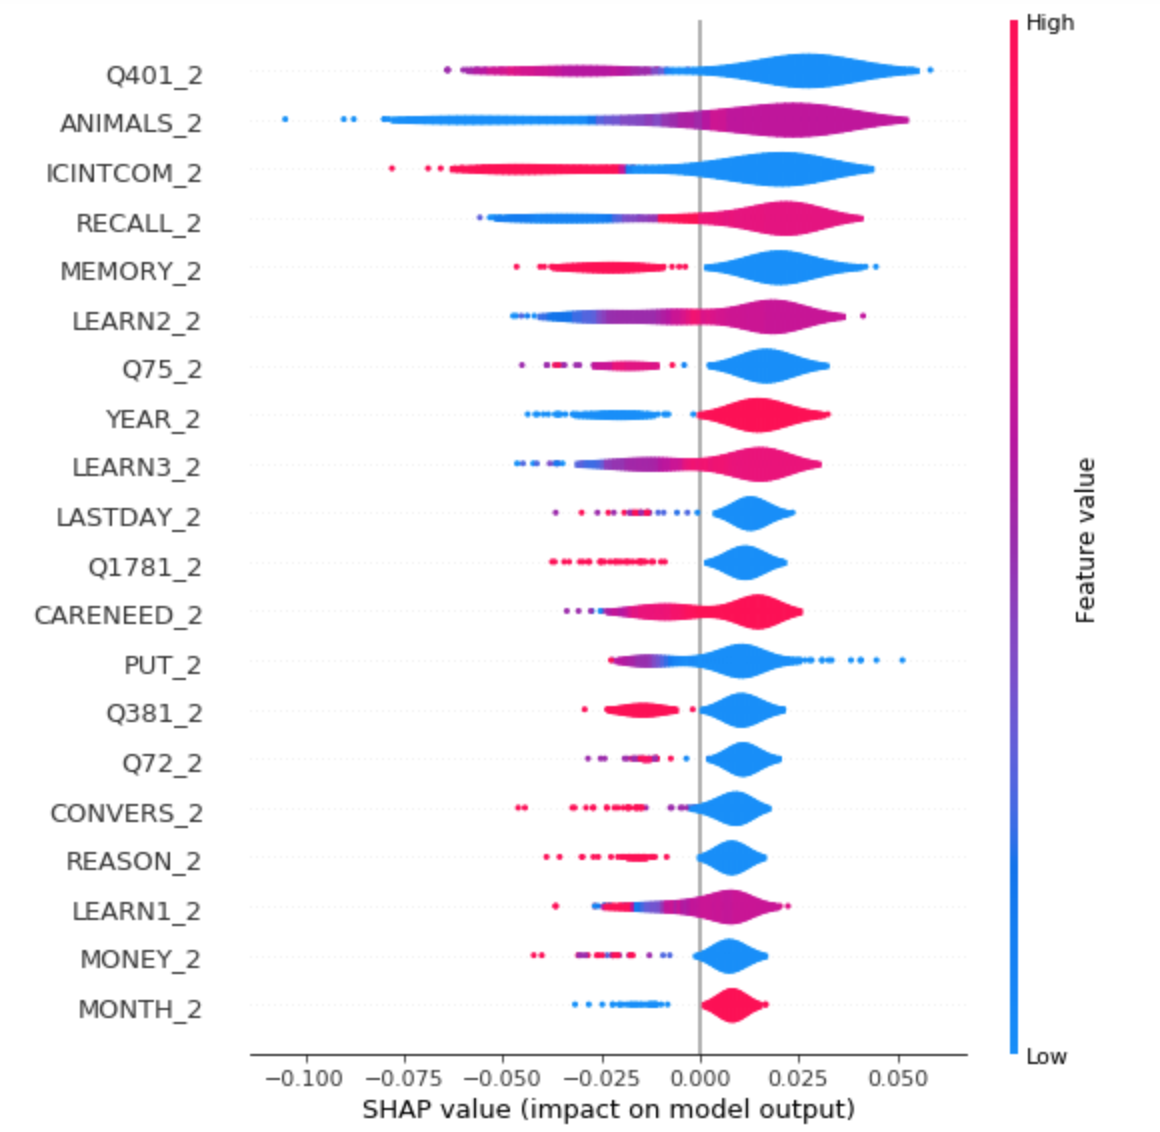
\includegraphics[scale=0.5]{\detokenize{shap_plots/1.png}}
\caption{Class 0}
\end{figure}
\begin{figure}[H]
\centering
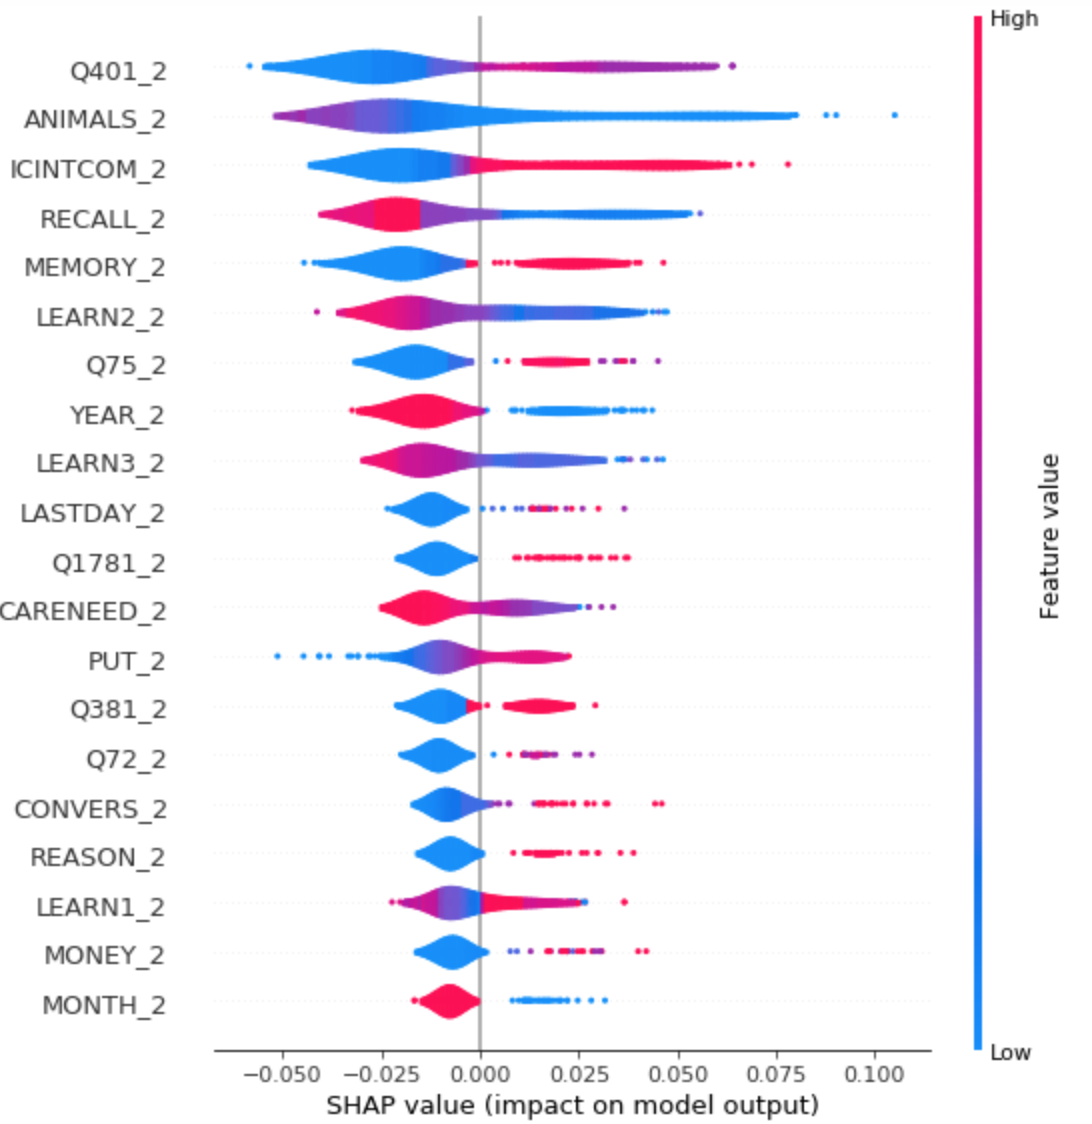
\includegraphics[scale=0.5]{\detokenize{shap_plots/2.png}}
\caption{Class 1}
\end{figure}
\subsection{Global SHAP Interaction Values}
\begin{figure}[H]
\centering
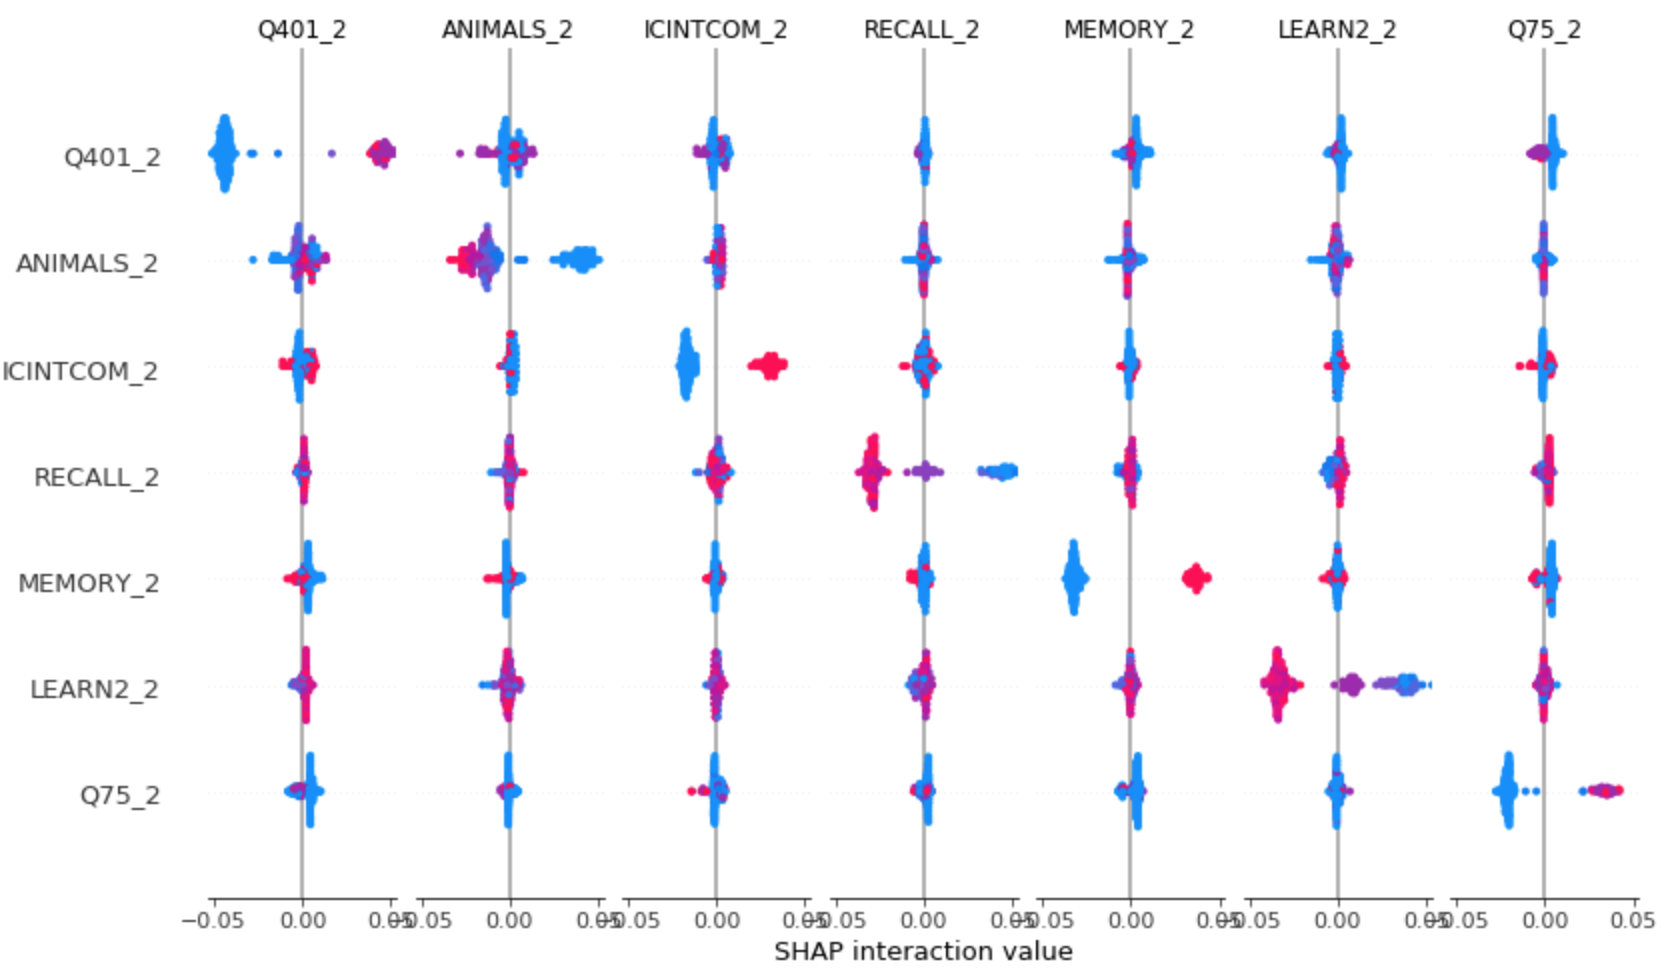
\includegraphics[scale=0.5]{\detokenize{shap_plots/3.png}}
\end{figure}
\subsection{Multi-output Decision Plot for properly classified Rows}
\begin{figure}[H]
\centering
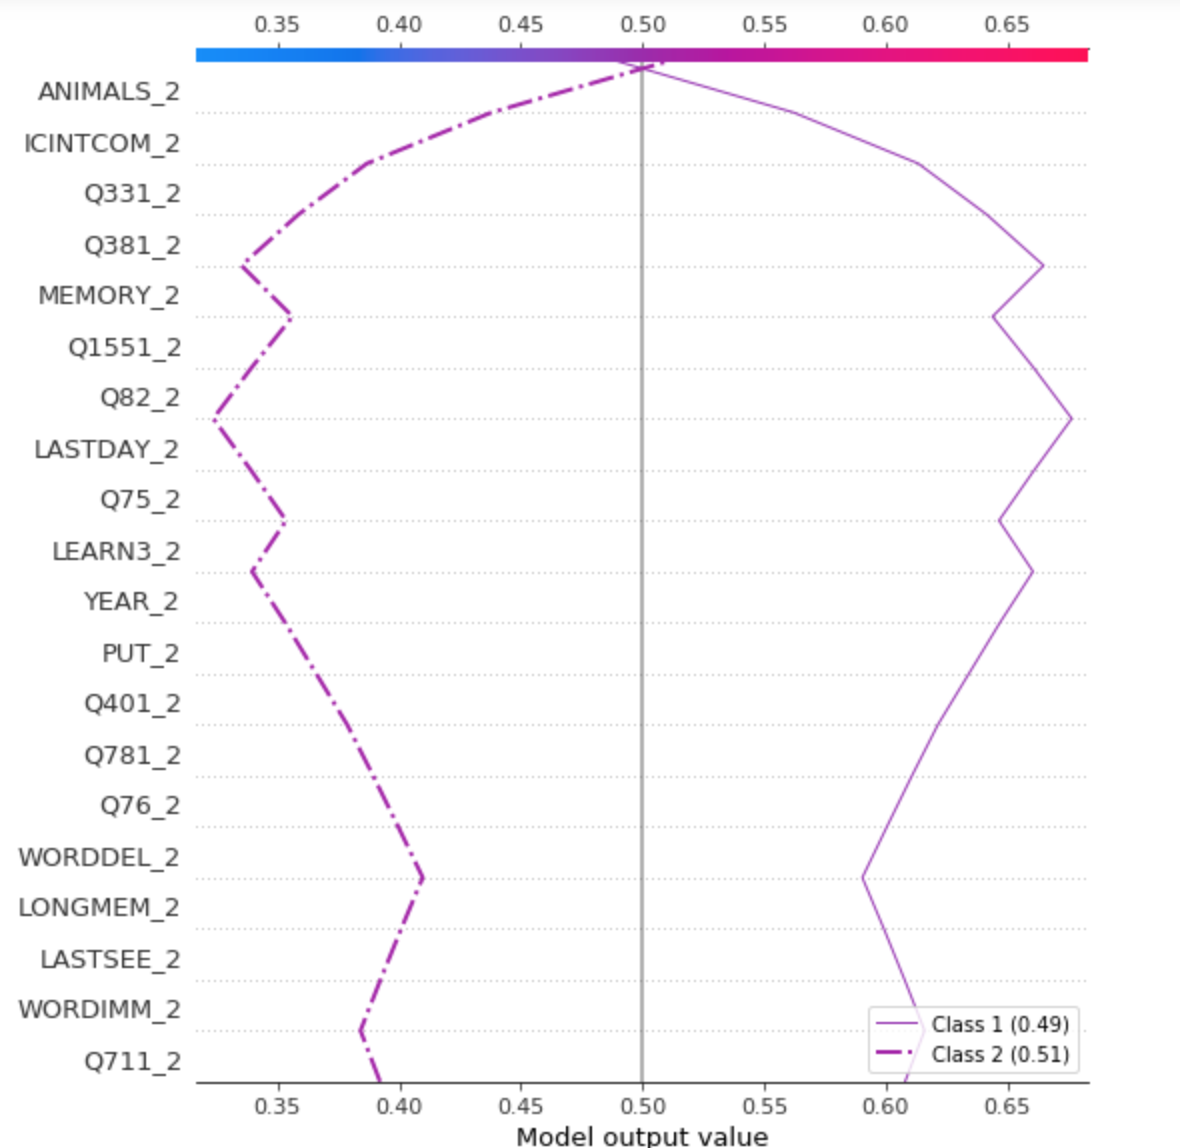
\includegraphics[scale=0.5]{\detokenize{shap_plots/4.png}}
\caption{Row with label = 0}
\end{figure}
\begin{figure}[H]
\centering
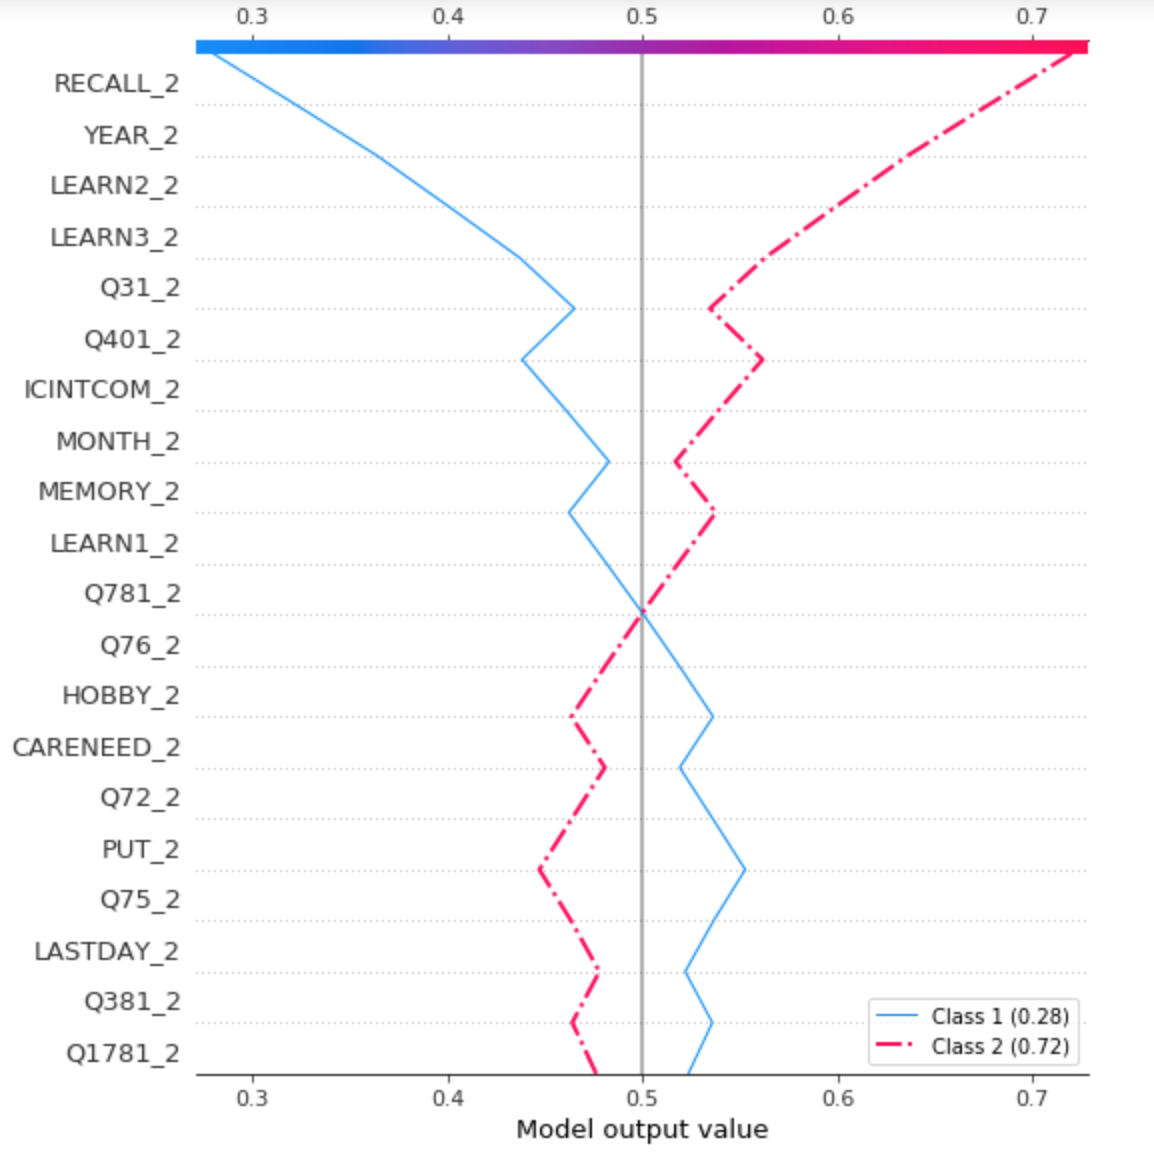
\includegraphics[scale=0.5]{\detokenize{shap_plots/5.png}}
\caption{Row with label = 1}
\end{figure}
\subsection{Decision Plot for Miss-classified Row}
\begin{figure}[H]
\centering
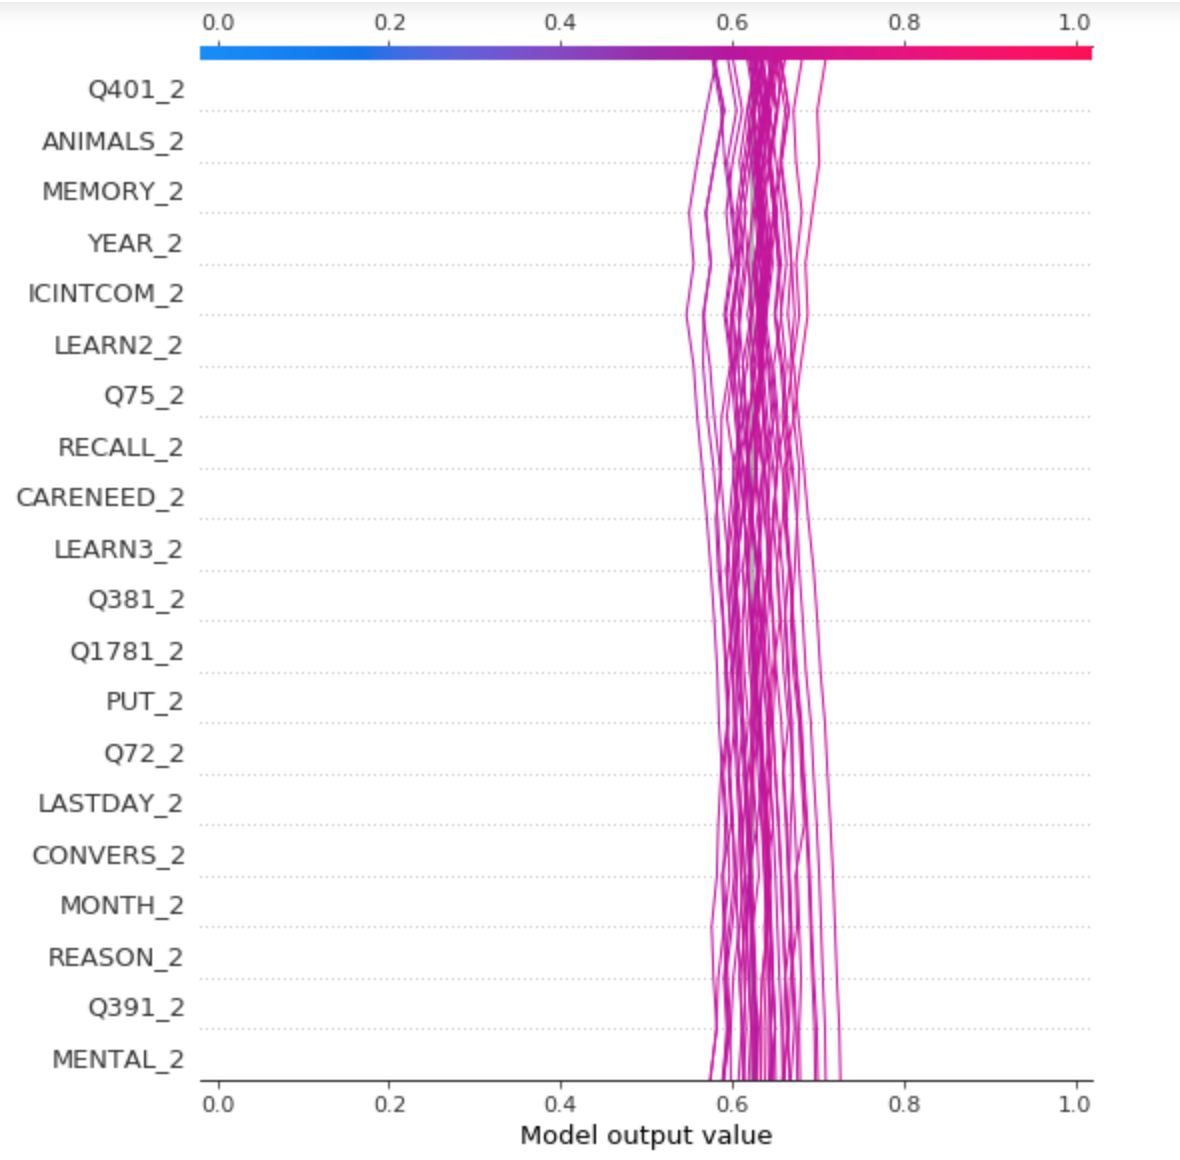
\includegraphics[scale=0.5]{\detokenize{shap_plots/6.png}}
\end{figure}

\section{Chapter 6: Precision, Recall, and F-measure}
The chapter summarizes the precision, recall, and f-measures of multiclass and binary classification for the case of balanced data.

\section{Chapter 7:ROC Curves and Precision-Recall
Curves}
ROC Curves (receiver operating characteristic curve) and ROC AUC (area under the ROC curve) are used to decide if the model differentiates between the labels. 
\subsection{ROC Curve}
The threshold is applied to the cut point in probability between the positive and negative classes. In order to decide on the best threshold, we evaluate the true positive and false positives for different threshold values, a curve can be constructed that stretches from the bottom left to top right and bows toward the top left. This curve is called the ROC curve. A classifier that has no discriminative power between positive and negative classes will form a diagonal line between (0,0) and (1,1). Models represented by points below this line have worse than no skill.
\subsection{AUC}
Area under the curve is calculated to give a single score for a classifier model across all threshold values. This is called the ROC area under curve or ROC AUC or sometimes ROCAUC. The score is a value between 0.0 and 1.0, with 1.0 indicating a perfect classifier.
\section{Chapter 8: Probability Scoring Methods}
\subsection{Probability Metrics}
On some problems, a crisp class label is not required, and instead a probability of class membership is preferred. The probability summarizes the likelihood (or uncertainty) of an example belonging to each class label. 
\subsection{LogLoss Score}
Logarithmic loss or log loss for short is a loss function known for training the logistic regression classification algorithm. The log loss function calculates the negative log likelihood for probability predictions made by the binary classification model. Most notably, this is logistic regression,but this function can be used by other models, such as neural networks, and is known by other names, such as cross-entropy.
\section{Cross Validation for Imbalanced Datasets}
The solution is to not split the data randomly when using k-fold cross-validation or a train-test split. Specifically, we can split a dataset randomly, although in such a way that maintains the same class distribution in each subset. This is called stratification or stratified sampling and the target variable (y), the class, is used to control the sampling process. This is available using sklearn stratified kfold.
\section{Chapter 10}
Summarizes oversampling and undersampling techniques which are available in chapters 12 and 13 in details.
\section{Chapter 12}
\subsection{Oversampling}
All techniques available through the python library: imblearn.over\_sampling

\begin{itemize}
    \item Random Oversampling: simplest oversampling method, involves randomly duplicating examples from the minority class in the training dataset
    \item SMOTE (Synthetic Minority Oversampling Technique): works by selecting examples that are close in the feature space, drawing a line between the examples in the feature space and drawing a new sample as a point along that line
    \item Borderline-SMOTE: involves selecting those instances of the minority class that are misclassified, such as with a k-nearest neighbor classification model, and only generating synthetic samples that are difficult to classify. Borderline Oversampling is an extension to SMOTE that fits an SVM to the dataset and uses the decision boundary as defined by the support vectors as the basis for generating synthetic examples, again based on the idea that the decision boundary is the area where more minority examples are required.
    \item Adaptive Synthetic Sampling (ADASYN): another extension to SMOTE that generates synthetic samples inversely proportional to the density of the examples in the minority class. It is designed to create synthetic examples in regions of the feature space where the density of minority examples is low, and fewer or none where the density is high.
\end{itemize}
\subsection{Undersampling Techniques}
\begin{itemize}
    \item Random Undersampling
\end{itemize}
\section{Data Transforms (Hiyam)}
\subsection{Scaling Numeric Data (chapter 17)}
\begin{itemize}
\item Normalization (Min-Max Scaling)
\item Standardization
\end{itemize}

\subsection{Scaling Data with Outliers (chapter 18)}
Many machine learning algorithms perform better when \textbf{numerical} input variables are scaled. Standardization is a popular scaling technique that substracts the mean from the values and divide by the stadard deviation, transforming the probability distribution from for an input variable to a Standard Gaussian (zero mean and unit variance).

\noindent \textbf{Problem:} Standardization can become skewed or biased when the input variable contains outliers.

\subsubsection*{Robust Scaling}
When we are scaling the data, and if we have very large values relative to the other input variables, these large values can dominate or skew some machine learning algorithms. \textbf{The result is that the algorithms pay most of their attention on the large values and ignore the variables with smaller values}.

\noindent Outliers are values at the edge of the distribution that may have a low probability of occurence, yet are overrepresented for some reason. \textbf{Outliers can skew a probability distribution and make data scaling using standardization difficult as the calculated mean and standard deviation will be skewed by the presence of outliers.}

\noindent \textbf{Approach:} When standardizing input variables containing outliers, we can ignore outliers from the calculation of the mean and standard deviation, and use the calculated values to scale the data

\noindent \textbf{This is called robust standardization}. This can be achieved by calculating the median (50th percentile) and the 25th and 75th percentile. The values of each variable can then have their median subtracted and are divided by the inter quartile range (IQR) which is the difference between the 25th and 75th percentile.

\begin{equation}
value = \frac{value - median}{p_{75} - p_{25}}
\end{equation}

The resulting value has a \textbf{zero mean and median and a standard deviation of 1}. Although not skewed by outliers and the outliers are still present with the same relative relationships to other values.

\subsection{How to Encode Categorical Data (chapter 19)}
Machine learning models require all input and output variables to be numeric. This means that if the data contains categorical data, we must encode it to numbers before we fit and evaluate our models.

\subsection*{Ordinal Encoding}
Each unique category is assigned an integer value. Example: \textit{red} is 1, \textit{green} is 2, \textit{blue} is 3.

\noindent For categorical variables, it imposes and \textbf{ordinal relationship} when no such relationship exists. This may cause problems and \textbf{one hot encoding} may be used instead.

\subsection*{One Hot Encoding}
For categorical variable where no ordinal relationship exists, the ordinal encoding is not enough and may be misleading.

\noindent One Hot Encoding works by creating binary variables for each category. For Example: \textit{red} will be [1, 0, 0], \textit{blue} will be [0, 1, 0], and \textit{green} will be [0, 0, 1].

\subsection*{Dummy Variable Encoding}
The one hot encoding includes a binary representation for each category. This might cause redundancy. 

\noindent if we know that [1, 0, 0] represents \textit{blue}, and [0, 1, 0] represents \textit{green}, we don't need another binary variable to represent \textit{red}, instead we could use 0 values along, e.g. [0, 0]. This is called dummy variable encoding and always represents $C$ categories with $C-1$ binary variables.

\noindent Other being less redundant, it is required for some models.

\subsection{How to Make Distributions Look More Gaussian (chapter 20)}
Several Machine Learning Algorithms assume the numerical values have a Gaussian distribution. Our data may not have a Gaussian distribution and it might have a Gaussian-like distribution.

\section{Data Pre-Pocessing}
After we have filtered the legal features in our data, and we deleted the features that have $>$ 40 \% missing values, we are left out with 255 legal features. These features must be pre-processed before we do the modelling exercise, for the following reasons:
\begin{enumerate}
\item All the 255 legal features still have missing values
\item We have a combination of numeric, ordinal, and categorical features, whereby each might require a different kind of scaling
\end{enumerate}

\subsection{Imputing Missing Values - Categorical Features}
For \textbf{all} categorical features, we will impute missing values by adding \textbf{a new category} for missing values. This way, any value that is missing will have its own category(label)

\subsection{Imputing Missing Values - Numerical/Ordinal Features}
For all numeric/ordinal features, we will impute missing values using \textbf{KNN}.

\noindent \textcolor{blue}{We discussed in one of our meeting that we will treat ordinal features as numeric, that's why we considered treating ordinal as numeric features therefore they are also imputed using KNN}

\subsection{Scaling - Numeric/Ordinal Features}
We applied \textbf{Robust Scaling} for all numeric/ordinal features.

\noindent \textbf{Robust Scaling} is good for data that includes outliers, and all our features do have outliers (with a very low percentage, though). 

\noindent For more information about the \textbf{percentage of outliers/feature, please consult with the following dataframe on our github repository: \url{https://github.com/hiyamgh/dementia/blob/master/input/codebooks/erroneous_codebook_legal_outliers_filtered.csv}}

\subsection{Scaling - Categorical Features}
No scaling is applied for categorical features.


% \subsection{Imputation in Ordinal/Categorical Data}
% To be continued ... waiting to meet with Dr Khalil again. Some notes:
% \begin{enumerate}
%     \item We said we might do KNN and impute by getting the values from the nearest neighbors.
%     \item It is common that public health practitioners usually disregard features with greater than 25\% missing, and since we have features that have greater than 25\% missing, we got the \textbf{theme} of each feature, and if the feature belongs to a particular theme that might not be of vital importance for detecting dementia, we will dis-regard the feature by itself.  
% \end{enumerate}

% \subsection{Imputation Currently Done}
% Just for now, to get things going, we imputed all missing values by replacing with the majority

% \subsection{Scaling}
% We have said earlier that we have three data types in our features: \textit{\textbf{numeric, ordinal, and categorical.}}

% \begin{itemize}
%     \item For ordinal and numeric data, we will be using the \textbf{Robust scaling} mechanism due to the presence of outliers
%     \item For categorical data, we will not scale it as we will be applying \textbf{dummy variable encoding} 
% \end{itemize}


% \subsection{Encoding Data}
% \begin{itemize}
%     \item For ordinal features, we will be applying Ordinal Encoding, as it will maintain an order between feature values.
%     \item For categorical features, we apply dummy variable encoding that decreases redundancy of one hot encoding
% \end{itemize}


\section{Imputing Numerical Missing Data}
In this section, we will be listing the multiple imputation methods that may be used for imputing missing \textbf{numeric} data. \textcolor{blue}{I referred to the data preparation book we have}

\subsection{Statistical Imputation}
Using mean, median, mode, constant value

\subsection{K Nearest Neighbors}
K nearest neighbor model. A new sample is imputed by finding samples in the training set closest to it and averages these nearby points to fill in the value. Must specify the \textbf{distance} to use and the \textbf{number of neighbors} neeeded for imputation

\subsection{Iterative Imputation}
.  Iterative imputation refers to a process where each feature is modeled as a function of the other features, e.g.  a regression problem where missing values are predicted.  Each feature is imputed sequentially, one after the other,allowing prior imputed values to be used as part of a model in predicting subsequent features.It is iterative because this process is repeated multiple times, allowing ever improved estimates of missing values to be calculated as missing values across all features are estimated.  \textcolor{blue}{This approach may be generally referred to as fully conditional specification (FCS) or multivariate imputation by chained equations (MICE)}.

\section{Imputing Categorical Missing Data}
In this section, we will be listing the multiple imputation methods that may be used for imputing missing \textbf{categorical} data

\section*{Single based Imputation Methods}

\subsection{Mean Imputation}
The mean imputation replaces missing values with the observed mean of the available data.

\subsection{Imputation Using Most Frequent or (Zero/Constant Values)}
Most Frequent is another statistical strategy to impute missing values and it works with categorical features (strings or numerical representations) by replacing missing data with the most frequent values within each column

\subsection{Create a New Category (Random Category) for NAN Values}
\textcolor{blue}{I think its more of a "hack" rather than an actual imputation method}

\subsection{ Adding a Variable To Capture NAN}
Replace NAN categories with most occurred values, and add a new feature to introduce some weight/importance to non-imputed and imputed observations. Create a new column and replace 1 if the category is NAN else 0. This column is an importance column to the imputed category.Replace NAN value with most occurred category in the actual column.

\subsection{Imputation Using Deep Learning (Datawig)}
\textcolor{blue}{Its actually a repository for AWS -- DataWig learns Machine Learning models to impute missing values in tables. -- So not sure how trustworthy it is}
This method works very well with categorical and non-numerical features. It is a library that learns Machine Learning models using Deep Neural Networks to impute missing values in a dataframe. It also supports both CPU and GPU for training.

\subsection{Regression Imputation}
\textcolor{blue}{The resource I used mentions this under the imputation for categorical variables, unless they treat each category as a \textbf{regressor variable}(numeric) but in my humble opinion, I think it can be used as a classification (in case we want to predict a category rather than a numeric outcome)?}
Regression Imputation consists of using some selected prediction of a missing value  on a variable of interest. For instance, to predict the missing value for the variable, say $X_1$, use this variable as a function of other variables, say $X_2$ and $X_3$ in a model that could even include the dependent variable $Y$

\textbf{Cons:} The \textbf{uncertainty} is not incorporated very well because the estimates are random variables.

\subsection{Imputation Using Interpolation}
\textcolor{blue}{I think this might fit if the data is time series but I'm not sure if it can be used in non-time series data} Suppose a varoable $X$ is measured at times $t = 1, 2, 3 (X_1, X_2, and X_3)$ and some values are missing at $t=2 (X_2)$, then $X_2 = \frac{X_1 + X_3}{2}$

\subsection*{Multiple Imputation}
Single based Imputation Methods mentioned earlier are an improvement over the case deletion method, but they do not account for the uncertainty in the imputations as imputed values are treated as true rather than estimates of the missing values leading to the under estimation of the variance of the estimates and the distortion of relationships among variables.Goal of \textbf{multiple imputation} is to account for uncertainty in imputed values. This method uses a selected model, such as a regression model to predict missing values on a variable. Instead of picking one value for the missing value, many values are chosen and the uncertainty is presented in the variance covariance matrix.

\subsection{Multivariate Normal Imputation (MNVI)}
\begin{itemize}
\item MNVI assumes all variables in the model are normally distributed \textcolor{blue}{problem for us?}
\item uses Markov Chain Monte Carlo Procedure to obtained imputed values from estimated multivariate distribution allowing uncertainty
\end{itemize}

\subsection{Multiple Imputation by Chained Equations (MICE)}
This type of imputation works by filling the missing data multiple times. The chained equations approach is also very flexible and can handle different variables of different data types (ie., continuous or binary) as well as complexities such as bounds or survey skip patterns. 

\subsection*{Other Imputation Methods}
\subsection{Stochastic regression imputation:}
It is quite similar to regression imputation which tries to predict the missing values by regressing it from other related variables in the same dataset plus some random residual value.

\subsection{Extrapolation and Interpolation:}
It tries to estimate values from other observations within the range of a discrete set of known data points.

\subsection{Hot-Deck Imputation}
Works by randomly choosing the missing value from a set of related and similar variables.

\subsection{Some papers for handling missing categorical data (did not read them at length -- just the abstract)}

\begin{itemize}
\item \href{https://www.sciencedirect.com/science/article/abs/pii/S0164121216301583?casa_token=ZELiCdTNfw4AAAAA:_dpjT3fvcxOkRXX1po7HaCnzb02biPjrKEYw-j8d7OU_krEYFqaaQIIwQo3rki5tbUWitsJstA}{Combining instance selection for better missing value imputation}
\item \href{https://link.springer.com/article/10.1007/s10115-019-01427-1}{Missing data imputation using decision trees and fuzzy clustering with iterative learning}
\item \href{https://www.sciencedirect.com/science/article/abs/pii/S0925231216309407?casa_token=dC_ROkr-pWoAAAAA:s5zwIWUilFRt2zbv5YcFVu6kzsNhdZN3c_OfUpQ1s1e-f9-c4VqcB1_OnXS-kGF0-kPzctFJ9A}{Probabilistic neural network based categorical data imputation}
\end{itemize}

\subsection*{References}
\begin{itemize}
\item \url{https://projecteuclid.org/download/pdfview_1/euclid.bjps/1481619615}

\item \url{http://www.jds-online.com/files/JDS-612.pdf}

\item\url{ https://towardsdatascience.com/6-different-ways-to-compensate-for-missing-values-data-imputation-with-examples-6022d9ca0779}
\item \url{https://github.com/awslabs/datawig}
\item \url{https://medium.com/analytics-vidhya/ways-to-handle-categorical-column-missing-data-its-implementations-15dc4a56893}
\end{itemize}




\section{Plan for the Paper}
\begin{enumerate}
\item Fix roaa’s code
\item MAML with random sampling, Reptile with random sampling
\item MAML with FP growth, Reptile with FP growth
\item MAML with ARML, Reptile with ARML
\item Ensure process is thorough with hyperparameter search documented, winning hyper-parameters documented, and performance metrics cast against the baseline model
\item Quantitative Comparison between baseline ML, vanilla ML, metalearning in three sampling procedures
\item 
Qualitative Comparison between baseline ML, vanilla ML, metalearning in three sampling procedures
\end{enumerate}


\section{MAML - Sampling Training/Testing Tasks}
The MAML code is divided into a main method that calls the appropriate training and testing methods. Each method, will appropriately call the data generator component, which is responsible for generating the tasks that the meta learner uses for training and testing respectively. \textbf{The data generation process depends on the following hyper parameters:}
\begin{itemize}
\item \textit{meta\_batch\_size:} Number of tasks sampled per meta-update
\item \textit{update\_batch\_size:} Number of tasks samples per meta-update
\item \textit{num\_classes:} number of classes we are classifying
\end{itemize}

\noindent\textbf{The data generator component takes in two parameters as input:}
\begin{itemize}
\item \textit{num\_samples\_per\_class:} number of samples (i.e. data instances) to sample per classification class. (i.e. how many data samples we will take from each class. If $\text{num\_samples\_per\_class}= 32$, then, we will take 32 samples from class 0, and 32 samples from class 1. Notice this is a \textbf{stratified} sampling.)
\item \textit{batch\_size:} the batch size, whereby each mini-batch will contain the appropriate number of samples. 
\end{itemize}

\noindent\textbf{Note (Very Important):} Each mini-batch (from "\textit{batch\_size}") will contain  $  \text{num\_classes} * \text{num\_samples\_per\_class}$ data samples. The main method in the original MAML code that was public on github (which we took and adapted changes as appropriate) \footnote{\url{https://github.com/cbfinn/maml}} called the Data Generator component by setting the data generation parameters parameters to be equal to the following:
\begin{itemize}
\item $\text{num\_samples\_per\_class} = \text{update\_batch\_size} * 2$
\item $\text{batch\_size} = \text{meta\_batch\_size}$
\end{itemize}

\subsection*{Meta-Training}
\noindent Therefore, if for example we have $\text{meta\_batch\_size} = 16$ and $\text{update\_batch\_size}=16$, then the $\text{batch\_ size} = 16 $ \& $\text{num\_samples\_per\_class} = 16 * 2 = 32$. By that, since each mini-batch will have $n\text{num\_samples\_per\_class}$ number of data samples, then we have in total $16 * 32 = 512$ data samples used for training, and $512$ samples \textbf{for each class}, therefore, a total of $512 + 512 = 1024$ samples.

\subsection*{Support \& Query Sets}
We have seen in the example above that we had 1024 (16 batch size, 32 samples per class, 2 classes) training samples. These are distributed into \textit{support and query sets}. 

\noindent Similar to the idea of training, validation, and testing in a regular supervised learning exercise, here in meta learning, the support set is what the meta learner trains on, and the query set is what the meta learner validates on.

\noindent Each mini-batch will contain a support set, and a query set. Mini-batch is called an \textbf{\textit{episode}}. Since each episode contains 64 samples in total (32 for each class), those 64 samples, are further distributed between support and query sets. The support will take 32 samples and the query will take 32 samples (stratified distribution).

\subsection*{N-way K-shot}
The number of classes in the support set, is referred to as \textit{N-way} task, and the number of samples per class is referred to as \textit{K-shot}. Therefore, our task is a \textit{\textbf{2-way 32-shot classification task}} 


\subsection*{How Do We Evaluate Testing Predictions ?}
In the MAML inner loop, we calculate the gradient updates of all weights and pass the updated weights to the model to get the new prediction. The query dataset is used to get the task losses after each gradient update. However, we do multiple gradient updates, and this is controlled by the parameter $num\_inner\_updates$ \footnote{\url{https://cs330.stanford.edu/material/cs330_hw2.pdf}}. Therefore, when we report the testing error metrics, we report the performance on the support set and the performance on the query set. Since the query set is used in while doing gradient updates, and since we do that "$num\_inner\_updates$" times, we report the performance averaged across those "$num\_inner\_updates$" for the query set. 

 
\noindent In other terms, we have 1024 (16 meta batch size, 32 examples per class, 2 classes) distributed as 512 support set samples, and 512 query set samples. However, the 512 samples are tested $\text{num\_test\_updates} = 10$ times, \textbf{therefore, we are reporting the average of the support set + the 10 query set updates.}


\section{MAML vs Shallow Models - Dementia Dataset}

\subsection{Cost Sensitive Learning in Neural Networks}
We have many types of cost sensitive learning, here, we will be focusing on two types which are \textbf{weighting} and \textbf{miss-classification error/cost matrix}.

It is important to note that, after the input is forwarded from the input layer to the output layer, the neural network computes the \textbf{loss} which quantifies how much mistake did it make, if any. 

\subsection*{Key defenition - Loss}
The loss function in case of regression is the \textbf{mean squared error}, whilst that for classification is the \textbf{cross entropy loss} (binary cross entropy (for binary classification tasks) or categorical cross entropy for multi-classification tasks)

\subsection*{Key defenition - Logits}
Loss if computed on the \textbf{logits}. Logits are the raw outputs of the last layer of the neural network. Logits interpreted to be the unnormalised (or not-yet normalised) predictions (or outputs) of a model. These can give results, but we don't normally stop with logits, because interpreting their raw values is not easy.

Let's demonstrate this through an example, say we want to classify images as being either a cat or a dog. For the first new image, we get logit values out of 16.917 for a cat and then 0.772 for a dog. Higher means better, or ('more likely'), so we'd say that a cat is the answer. The correct answer is a cat, so the model worked. If we apply softmax activation to the logits, we get p(cat) = 0.99 and p(dog) = 0.0001

\subsection*{Weighting}
Weighting is applied to the loss such that smaller weight values result in errors, i.e. less update the model coefficients and larger weight results in more errors, i.e. more updates to the model coefficients.

\textbf{Multiply the logit with a weight vector representing scaling factor of each class}. 

\subsection*{Miss-Classification Errros/Cost-Matrix}
The problem with class weighting is that it applies the weighting to all the data that belongs to the class, whilst we want it to depend on the miss classification error.

\begin{table}[H]
\centering
\begin{tabular}{|l|l|l|}
\hline
actual/predicted & class 0 & class 1 \\ \hline
class 0          & 0       & 0.25    \\ \hline
class 1          & 0.25    & 0       \\ \hline
\end{tabular}
\caption{cost matrix of classifications/miss-classifications}
\end{table}

The table above shows that the cost of miss-classifying class 0 as class 1 or classifying class 1 as class 0 is 0.25 while correct classifications have no cost.

%%%%%%%%%%%%%%%%%%%%%%% Hyper Parameter Space %%%%%%%%%%%%%%%%%%
\subsection{Hyper Parameters}
In this section, we will be displaying the set of all \textbf{meta learning} related hyper parameters in comparison to the values chosen by the authors of MAML in their experiments:

\begin{table}[H]
%\resizebox{.7\width}{!}
{\begin{tabular}{|l|l|l|l|l|l|l|l|}
\hline
\multicolumn{1}{|c|}{\multirow{2}{*}{\textbf{Hyper Parameter}}}                                  & \multicolumn{1}{c|}{\multirow{2}{*}{\textbf{\begin{tabular}[c]{@{}c@{}}Range of \\ Values (Ours)\end{tabular}}}} & \multicolumn{4}{c|}{\textbf{Omniglot}}                                                                                                                                                                                                                                                                                                                          & \multicolumn{2}{c|}{\textbf{MiniImagenet}}                                                                                                                                    \\ \cline{3-8}
\multicolumn{1}{|c|}{}                                                                           & \multicolumn{1}{c|}{}                                                                                            & \multicolumn{1}{c|}{\textbf{\begin{tabular}[c]{@{}c@{}}5-way \\ 1-shot\end{tabular}}} & \multicolumn{1}{c|}{\textbf{\begin{tabular}[c]{@{}c@{}}5-way\\  5-shot\end{tabular}}} & \multicolumn{1}{c|}{\textbf{\begin{tabular}[c]{@{}c@{}}20-way \\ 1-shot\end{tabular}}} & \multicolumn{1}{c|}{\textbf{\begin{tabular}[c]{@{}c@{}}20-way\\  5-shot\end{tabular}}} & \multicolumn{1}{c|}{\textbf{\begin{tabular}[c]{@{}c@{}}5-way\\  1-shot\end{tabular}}} & \multicolumn{1}{c|}{\textbf{\begin{tabular}[c]{@{}c@{}}5-way\\  5-shot\end{tabular}}} \\ \hline
\begin{tabular}[c]{@{}l@{}}gradient steps - training\\ (num\_updates)\end{tabular}               & 4                                                                                                                & 1                                                                                     & 1                                                                                     & 5                                                                                      & 5                                                                                      & 5                                                                                     & 5                                                                                     \\ \hline
gradient steps - evaluation                                                                      & 10                                                                                                               & 3                                                                                     & 3                                                                                     & 5                                                                                      & 5                                                                                      & 10                                                                                    & 10                                                                                    \\ \hline
\begin{tabular}[c]{@{}l@{}}step size (alpha) - \\ update learning rate\end{tabular}              & 0.1, 0.001                                                                                                       & 0.4                                                                                   & 0.4                                                                                   & 0.1                                                                                    & 0.1                                                                                    & 0.01                                                                                  & 0.01                                                                                  \\ \hline
\begin{tabular}[c]{@{}l@{}}meta step size (beta) \\ - meta learning rate\end{tabular}            & 0.1, 0.001                                                                                                       & 0.001                                                                                 & 0.001                                                                                 & 0.001                                                                                  & 0.001                                                                                  & 0.001                                                                                 & 0.001                                                                                 \\ \hline
meta batch size                                                                                  & 4, 8, 16                                                                                                         & 32                                                                                    & 32                                                                                    & 16                                                                                     & 16                                                                                     & 4                                                                                     & 2                                                                                     \\ \hline
\begin{tabular}[c]{@{}l@{}}update batch size - K\\ (number of examples per\\ class)\end{tabular} & 4, 8, 16                                                                                                         & 1                                                                                     & 5                                                                                     & 1                                                                                      & 5                                                                                      & 1                                                                                     & 5                                                                                     \\ \hline
meta train iterations                                                                            & 1000                                                                                                             & 60000                                                                                 & 60000                                                                                 & 60000                                                                                  & 60000                                                                                  & 60000                                                                                 & 60000                                                                                 \\ \hline
\end{tabular}
}}
\caption{Hyper Parameter Space Containing all Meta-Learning Related Hyper Parameters}
\label{Tab:maml_meta_learning_hyperparameters}
\end{table}

\begin{table}[H]
%\resizebox{.7\width}{!}
{\begin{tabular}{|l|l|l|}
\hline
\multicolumn{3}{|l|}{\textbf{Base Learner Hyper Parameters}}                                                                                                                                                            \\ \hline
hidden layers                                  & the number of hidden layers and their nodes               & \begin{tabular}[c]{@{}l@{}}264, 128, 64\\ 128, 64, 64\\ 128, 64\\ 128\end{tabular}                         \\ \hline
activation functions                           & non-linear activation functions                           & \begin{tabular}[c]{@{}l@{}}relu, sigmoid, tanh, \\ softmax, swish\end{tabular}                             \\ \hline
\multicolumn{3}{|l|}{\textbf{Cost Sensitive Hyper Parameters}}                                                                                                                                                          \\ \hline
weights                                        & weights vector applied to logits                          & \begin{tabular}[c]{@{}l@{}}{[}1, 10{]}, {[}1, 100{]}, {[}1,1{]}, \\ {[}10, 1{]}, {[}100, 1{]}\end{tabular} \\ \hline
sampling strategy                              & sampling strategy used for under/over - sampling the data & \begin{tabular}[c]{@{}l@{}}minority, majority, all\\ 0.5, 0.75, 1\end{tabular}                             \\ \hline
\multicolumn{3}{|l|}{\textbf{FP Growth Hyper parameters}}                                                                                                                                                               \\ \hline
minimum support                                & minumum support for frequent patterns                     & 0.7, 0.8, 0.9                                                                                              \\ \hline
\multicolumn{3}{|l|}{\textbf{Other Hyper parameters}}                                                                                                                                                               
\\ \hline
encoding & categorical encoding mechanism &  \begin{tabular}[c]{@{}l@{}} catboost, glmm,\\ target, mestimator,\\ james, woe \end{tabular}                        
\\ \hline
\end{tabular}}}
\caption{Hyper Parameter Space Containing all other Hyper Parameters related to Base Model, Cost Sensitive Learning, and Categorical Encoding}
\label{Tab:maml_other_hyperparameters}
\end{table}

It is important to note that:
\begin{enumerate}
\item \textbf{step size $\alpha$:} is represented as the \textbf{step size (alpha) - update learning rate} in Table \ref{Tab:maml_meta_learning_hyperparameters} above.
\item \textbf{meta step size $\beta$:} is represented as the \textbf{meta step size - meta learning rate} in Table \ref{Tab:maml_meta_learning_hyperparameters} above.
\item \textbf{K}: the number of samples $K$ denoting N-way K-shot classification is represented as the \textbf{update batch size - K (number of examples per class)} in Table \ref{Tab:maml_meta_learning_hyperparameters} above
\end{enumerate}


%%%%%%%%%%%%%%%%%%%%%%% Winning Hyper Parameters %%%%%%%%%%%%%%%%%%
\subsection{Winning Hyper Parameters}
In Tables \ref{Tab:winning_with_top10},\ref{Tab:winning_with_top20},\ref{Tab:winning_without_top10}, and \ref{Tab:winning_without_top20} below, we display the winning hyper parameters for the top 20 best MAML models trained and tested on dementia top 10 and top 20 columns selected by feature selection, with and without including sampling with frequent patterns, respectively. Each table contains the following information:
\begin{itemize}
\item \textbf{model:} the name of the winning model
\item \textbf{miter:} the meta training iterations 
\item \textbf{mbs:} the meta batch size
\item \textbf{mlr:} the meta learning rate
\item \textbf{ulr:} the update learning rate
\item \textbf{dh:} dimensions hidden, i.e. the number of hidden layers and the number of nodes in each hidden layer. For example: \textit{128, 64} means that we have 2 hidden layers, the first having 128 nodes and the second having 64 nodes.
\item \textbf{afn:} activation function.
\item \textbf{nu:} number of testing updates. This is used by the meta learning code to repeat the evaluation on the query set, so here in this case, we evaluate the same query set 4 times for checking the generality of the results.
\item \textbf{ifp:} a boolean variable of whether we are including sampling with frequent patterns or not. 1 means we are, 0 means we are not.
\item \textbf{fp\_supp:} the minimum support used for discovering the frequent patterns.
\item \textbf{encoding:} The categorical encoding mechanism applied for the categorical columns in the data
\end{itemize}


% winning - with fp - top 10
\begin{table}[H]
\resizebox{.7\width}{!}{\begin{tabular}{|l|l|l|l|l|l|l|l|l|l|l|l|l|}
\hline
\textbf{model} & \textbf{miter} & \textbf{mbs} & \textbf{mlr} & \textbf{ulr} & \textbf{dh} & \textbf{afn} & \textbf{nu} & \textbf{ifp} & \textbf{fp\_supp} & \textbf{weights} & \textbf{sampling\_strategy} & \textbf{encoding} \\ \hline
model\_234     & 1000           & 16           & 0.1          & 0.1          & 128, 64     & relu         & 4           & 1            & 0.9               & 1, 10            & all                         & woe               \\ \hline
model\_487     & 1000           & 16           & 0.1          & 0.1          & 128, 64     & relu         & 4           & 1            & 0.7               & 10, 1            & 0.5                         & catboost          \\ \hline
model\_37      & 1000           & 16           & 0.1          & 0.1          & 128, 64     & relu         & 4           & 1            & 0.8               & 1, 10            & minority                    & catboost          \\ \hline
model\_471     & 1000           & 16           & 0.1          & 0.1          & 128, 64     & relu         & 4           & 1            & 0.7               & 10, 1            & minority                    & target            \\ \hline
model\_469     & 1000           & 16           & 0.1          & 0.1          & 128, 64     & relu         & 4           & 1            & 0.7               & 10, 1            & minority                    & catboost          \\ \hline
model\_529     & 1000           & 16           & 0.1          & 0.1          & 128, 64     & relu         & 4           & 1            & 0.7               & 100, 1           & 1                           & catboost          \\ \hline
model\_490     & 1000           & 16           & 0.1          & 0.1          & 128, 64     & relu         & 4           & 1            & 0.7               & 10, 1            & 0.5                         & mestimator        \\ \hline
model\_73      & 1000           & 16           & 0.1          & 0.1          & 128, 64     & relu         & 4           & 1            & 0.8               & 1, 100           & minority                    & catboost          \\ \hline
model\_409     & 1000           & 16           & 0.1          & 0.1          & 128, 64     & relu         & 4           & 1            & 0.7               & 1, 10            & all                         & catboost          \\ \hline
model\_60      & 1000           & 16           & 0.1          & 0.1          & 128, 64     & relu         & 4           & 1            & 0.8               & 1, 10            & 0.5                         & woe               \\ \hline
model\_62      & 1000           & 16           & 0.1          & 0.1          & 128, 64     & relu         & 4           & 1            & 0.8               & 1, 10            & 1                           & glmm              \\ \hline
model\_308     & 1000           & 16           & 0.1          & 0.1          & 128, 64     & relu         & 4           & 1            & 0.9               & 10, 1            & 0.5                         & glmm              \\ \hline
model\_292     & 1000           & 16           & 0.1          & 0.1          & 128, 64     & relu         & 4           & 1            & 0.9               & 10, 1            & minority                    & mestimator        \\ \hline
model\_353     & 1000           & 16           & 0.1          & 0.1          & 128, 64     & relu         & 4           & 1            & 0.9               & 100, 1           & 1                           & james             \\ \hline
model\_492     & 1000           & 16           & 0.1          & 0.1          & 128, 64     & relu         & 4           & 1            & 0.7               & 10, 1            & 0.5                         & woe               \\ \hline
model\_70      & 1000           & 16           & 0.1          & 0.1          & 128, 64     & relu         & 4           & 1            & 0.8               & 1, 10            & 0.75                        & mestimator        \\ \hline
model\_450     & 1000           & 16           & 0.1          & 0.1          & 128, 64     & relu         & 4           & 1            & 0.7               & 1, 100           & all                         & woe               \\ \hline
model\_303     & 1000           & 16           & 0.1          & 0.1          & 128, 64     & relu         & 4           & 1            & 0.9               & 10, 1            & all                         & target            \\ \hline
model\_262     & 1000           & 16           & 0.1          & 0.1          & 128, 64     & relu         & 4           & 1            & 0.9               & 1, 100           & not minority                & mestimator        \\ \hline
model\_408     & 1000           & 16           & 0.1          & 0.1          & 128, 64     & relu         & 4           & 1            & 0.7               & 1, 10            & not minority                & woe               \\ \hline
\end{tabular}}}
\caption{Winning Hyper Parameters - MAML with FP, using top 10 columns}
\label{Tab:winning_with_top10}
\end{table}

% winning - with fp - top 20
\begin{table}[H]
\resizebox{.7\width}{!}{\begin{tabular}{|l|l|l|l|l|l|l|l|l|l|l|l|l|}
\hline
\textbf{model} & \textbf{miter} & \textbf{mbs} & \textbf{mlr} & \textbf{ulr} & \textbf{dh} & \textbf{afn} & \textbf{nu} & \textbf{ifp} & \textbf{fp\_supp} & \textbf{weights} & \textbf{sampling\_strategy} & \textbf{encoding} \\ \hline
model\_663     & 1000           & 16           & 0.1          & 0.1          & 128         & relu         & 4           & 1            & 0.8               & 10, 1            & all                         & target            \\ \hline
model\_234     & 1000           & 16           & 0.1          & 0.1          & 128, 64     & relu         & 4           & 1            & 0.9               & 1, 10            & all                         & woe               \\ \hline
model\_582     & 1000           & 16           & 0.1          & 0.1          & 128         & relu         & 4           & 1            & 0.8               & 1, 10            & minority                    & woe               \\ \hline
model\_606     & 1000           & 16           & 0.1          & 0.1          & 128         & relu         & 4           & 1            & 0.8               & 1, 10            & 1                           & woe               \\ \hline
model\_317     & 1000           & 16           & 0.1          & 0.1          & 128, 64     & relu         & 4           & 1            & 0.9               & 10, 1            & 1                           & james             \\ \hline
model\_339     & 1000           & 16           & 0.1          & 0.1          & 128, 64     & relu         & 4           & 1            & 0.9               & 100, 1           & all                         & target            \\ \hline
model\_583     & 1000           & 16           & 0.1          & 0.1          & 128         & relu         & 4           & 1            & 0.8               & 1, 10            & not minority                & catboost          \\ \hline
model\_672     & 1000           & 16           & 0.1          & 0.1          & 128         & relu         & 4           & 1            & 0.8               & 10, 1            & 0.5                         & woe               \\ \hline
model\_318     & 1000           & 16           & 0.1          & 0.1          & 128, 64     & relu         & 4           & 1            & 0.9               & 10, 1            & 1                           & woe               \\ \hline
model\_678     & 1000           & 16           & 0.1          & 0.1          & 128         & relu         & 4           & 1            & 0.8               & 10, 1            & 1                           & woe               \\ \hline
model\_320     & 1000           & 16           & 0.1          & 0.1          & 128, 64     & relu         & 4           & 1            & 0.9               & 10, 1            & 0.75                        & glmm              \\ \hline
model\_243     & 1000           & 16           & 0.1          & 0.1          & 128, 64     & relu         & 4           & 1            & 0.9               & 1, 10            & 1                           & target            \\ \hline
model\_653     & 1000           & 16           & 0.1          & 0.1          & 128         & relu         & 4           & 1            & 0.8               & 10, 1            & minority                    & james             \\ \hline
model\_217     & 1000           & 16           & 0.1          & 0.1          & 128, 64     & relu         & 4           & 1            & 0.9               & 1, 10            & minority                    & catboost          \\ \hline
model\_323     & 1000           & 16           & 0.1          & 0.1          & 128, 64     & relu         & 4           & 1            & 0.9               & 10, 1            & 0.75                        & james             \\ \hline
model\_667     & 1000           & 16           & 0.1          & 0.1          & 128         & relu         & 4           & 1            & 0.8               & 10, 1            & 0.5                         & catboost          \\ \hline
model\_247     & 1000           & 16           & 0.1          & 0.1          & 128, 64     & relu         & 4           & 1            & 0.9               & 1, 10            & 0.75                        & catboost          \\ \hline
model\_580     & 1000           & 16           & 0.1          & 0.1          & 128         & relu         & 4           & 1            & 0.8               & 1, 10            & minority                    & mestimator        \\ \hline
model\_221     & 1000           & 16           & 0.1          & 0.1          & 128, 64     & relu         & 4           & 1            & 0.9               & 1, 10            & minority                    & james             \\ \hline
model\_322     & 1000           & 16           & 0.1          & 0.1          & 128, 64     & relu         & 4           & 1            & 0.9               & 10, 1            & 0.75                        & mestimator        \\ \hline
\end{tabular}}}
\caption{Winning Hyper Parameters - MAML with FP, using top 20 columns}
\label{Tab:winning_with_top20}
\end{table}


% winning - without fp - top 10
\begin{table}[H]
\resizebox{.7\width}{!}{\begin{tabular}{|l|l|l|l|l|l|l|l|l|l|l|l|}
\hline
\textbf{model} & \textbf{miter} & \textbf{mbs} & \textbf{mlr} & \textbf{ulr} & \textbf{dh} & \textbf{afn} & \textbf{nu} & \textbf{ifp} & \textbf{fp\_supp} & \textbf{weights} & \textbf{sampling\_strategy} \\ \hline
model\_134     & 1000           & 16           & 0.1          & 0.1          & 128, 64     & relu         & 4           & 1            & 0.9               & 1, 100           & not minority                \\ \hline
model\_120     & 1000           & 16           & 0.1          & 0.1          & 128, 64     & relu         & 4           & 1            & 0.8               & 100, 1           & 0.75                        \\ \hline
model\_226     & 1000           & 16           & 0.1          & 0.1          & 128         & relu         & 4           & 1            & 0.9               & 1, 100           & 0.5                         \\ \hline
model\_186     & 1000           & 16           & 0.1          & 0.1          & 128         & relu         & 4           & 1            & 0.8               & 1, 1             & 0.75                        \\ \hline
model\_194     & 1000           & 16           & 0.1          & 0.1          & 128         & relu         & 4           & 1            & 0.8               & 1, 100           & not minority                \\ \hline
model\_149     & 1000           & 16           & 0.1          & 0.1          & 128, 64     & relu         & 4           & 1            & 0.9               & 100, 1           & 1                           \\ \hline
model\_238     & 1000           & 16           & 0.1          & 0.1          & 128         & relu         & 4           & 1            & 0.9               & 100, 1           & 0.5                         \\ \hline
model\_115     & 1000           & 16           & 0.1          & 0.1          & 128, 64     & relu         & 4           & 1            & 0.8               & 100, 1           & minority                    \\ \hline
model\_205     & 1000           & 16           & 0.1          & 0.1          & 128         & relu         & 4           & 1            & 0.8               & 100, 1           & minority                    \\ \hline
model\_185     & 1000           & 16           & 0.1          & 0.1          & 128         & relu         & 4           & 1            & 0.8               & 1, 1             & 1                           \\ \hline
model\_228     & 1000           & 16           & 0.1          & 0.1          & 128         & relu         & 4           & 1            & 0.9               & 1, 100           & 0.75                        \\ \hline
model\_60      & 1000           & 16           & 0.1          & 0.1          & 128, 64, 64 & relu         & 4           & 1            & 0.9               & 100, 1           & 0.75                        \\ \hline
model\_486     & 1000           & 16           & 0.1          & 0.001        & 128         & relu         & 4           & 1            & 0.9               & 1, 1             & 0.75                        \\ \hline
model\_484     & 1000           & 16           & 0.1          & 0.001        & 128         & relu         & 4           & 1            & 0.9               & 1, 1             & 0.5                         \\ \hline
model\_201     & 1000           & 16           & 0.1          & 0.1          & 128         & relu         & 4           & 1            & 0.8               & 10, 1            & all                         \\ \hline
model\_191     & 1000           & 16           & 0.1          & 0.1          & 128         & relu         & 4           & 1            & 0.8               & 1, 10            & 1                           \\ \hline
model\_190     & 1000           & 16           & 0.1          & 0.1          & 128         & relu         & 4           & 1            & 0.8               & 1, 10            & 0.5                         \\ \hline
model\_22      & 1000           & 16           & 0.1          & 0.1          & 128, 64, 64 & relu         & 4           & 1            & 0.8               & 10, 1            & 0.5                         \\ \hline
model\_481     & 1000           & 16           & 0.1          & 0.001        & 128         & relu         & 4           & 1            & 0.9               & 1, 1             & minority                    \\ \hline
model\_116     & 1000           & 16           & 0.1          & 0.1          & 128, 64     & relu         & 4           & 1            & 0.8               & 100, 1           & not minority                \\ \hline
model\_209     & 1000           & 16           & 0.1          & 0.1          & 128         & relu         & 4           & 1            & 0.8               & 100, 1           & 1                           \\ \hline
\end{tabular}}}
\caption{Winning Hyper Parameters - MAML without FP, using top 10 columns}
\label{Tab:winning_without_top10}
\end{table}

% winning - without fp - top 20
\begin{table}[H]
\resizebox{.7\width}{!}{\begin{tabular}{|l|l|l|l|l|l|l|l|l|l|l|l|}
\hline
\textbf{model} & \textbf{miter} & \textbf{mbs} & \textbf{mlr} & \textbf{ulr} & \textbf{dh} & \textbf{afn} & \textbf{nu} & \textbf{ifp} & \textbf{weights} & \textbf{sampling\_strategy} & \textbf{encoding} \\ \hline
model\_144     & 1000           & 16           & 0.1          & 0.1          & 128, 64     & relu         & 4           & 0            & 10, 1            & 0.75                        & woe               \\ \hline
model\_324     & 1000           & 16           & 0.1          & 0.1          & 128         & relu         & 4           & 0            & 10, 1            & 0.75                        & woe               \\ \hline
model\_48      & 1000           & 16           & 0.1          & 0.1          & 128, 64     & relu         & 4           & 0            & 1, 10            & not minority                & woe               \\ \hline
model\_323     & 1000           & 16           & 0.1          & 0.1          & 128         & relu         & 4           & 0            & 10, 1            & 0.75                        & james             \\ \hline
model\_247     & 1000           & 16           & 0.1          & 0.1          & 128         & relu         & 4           & 0            & 1, 10            & 0.75                        & catboost          \\ \hline
model\_119     & 1000           & 16           & 0.1          & 0.1          & 128, 64     & relu         & 4           & 0            & 10, 1            & not minority                & james             \\ \hline
model\_302     & 1000           & 16           & 0.1          & 0.1          & 128         & relu         & 4           & 0            & 10, 1            & all                         & glmm              \\ \hline
model\_120     & 1000           & 16           & 0.1          & 0.1          & 128, 64     & relu         & 4           & 0            & 10, 1            & not minority                & woe               \\ \hline
model\_293     & 1000           & 16           & 0.1          & 0.1          & 128         & relu         & 4           & 0            & 10, 1            & minority                    & james             \\ \hline
model\_46      & 1000           & 16           & 0.1          & 0.1          & 128, 64     & relu         & 4           & 0            & 1, 10            & not minority                & mestimator        \\ \hline
model\_231     & 1000           & 16           & 0.1          & 0.1          & 128         & relu         & 4           & 0            & 1, 10            & all                         & target            \\ \hline
model\_70      & 1000           & 16           & 0.1          & 0.1          & 128, 64     & relu         & 4           & 0            & 1, 10            & 0.75                        & mestimator        \\ \hline
model\_399     & 1000           & 16           & 0.1          & 0.1          & 128, 64, 64 & relu         & 4           & 0            & 1, 10            & minority                    & target            \\ \hline
model\_243     & 1000           & 16           & 0.1          & 0.1          & 128         & relu         & 4           & 0            & 1, 10            & 1                           & target            \\ \hline
model\_122     & 1000           & 16           & 0.1          & 0.1          & 128, 64     & relu         & 4           & 0            & 10, 1            & all                         & glmm              \\ \hline
model\_285     & 1000           & 16           & 0.1          & 0.1          & 128         & relu         & 4           & 0            & 1, 100           & 0.75                        & target            \\ \hline
model\_239     & 1000           & 16           & 0.1          & 0.1          & 128         & relu         & 4           & 0            & 1, 10            & 0.5                         & james             \\ \hline
model\_116     & 1000           & 16           & 0.1          & 0.1          & 128, 64     & relu         & 4           & 0            & 10, 1            & not minority                & glmm              \\ \hline
model\_225     & 1000           & 16           & 0.1          & 0.1          & 128         & relu         & 4           & 0            & 1, 10            & not minority                & target            \\ \hline
model\_233     & 1000           & 16           & 0.1          & 0.1          & 128         & relu         & 4           & 0            & 1, 10            & all                         & james             \\ \hline
\end{tabular}}}
\caption{Winning Hyper Parameters - MAML without FP, using top 20 columns}
\label{Tab:winning_without_top20}
\end{table}


\subsection{Quantitative Results - Without FP Growth}

\subsubsection*{Without FP - Top 10 - F2 score}
% without fp - top 10 - f2
\begin{table}[H]
\resizebox{.7\width}{!}{\begin{tabular}{|l|l|l|l|l|l|l|l|l|l|l|l|l|}
\hline
\textbf{model} & \textbf{f2} & \textbf{gmean} & \textbf{bss} & \textbf{pr\_auc} & \textbf{sensitivity} & \textbf{specificity} & \textbf{ppv} & \textbf{accuracy} & \textbf{precision} & \textbf{recall} & \textbf{f1} & \textbf{auc} \\ \hline
model\_470     & 0.90878     & 0.76027        & 0.51269      & 0.69421          & 0.99056              & 0.53245              & 0.98625      & 0.76705           & 0.69604            & 0.99056         & 0.8128      & 0.76151      \\ \hline
model\_408     & 0.89015     & 0.76178        & 0.50741      & 0.70213          & 0.96014              & 0.56579              & 0.955839     & 0.76456           & 0.71013            & 0.96014         & 0.80897     & 0.76296      \\ \hline
model\_294     & 0.88917     & 0.72026        & 0.42943      & 0.66427          & 0.97911              & 0.46486              & 0.946201     & 0.72692           & 0.66781            & 0.97911         & 0.78746     & 0.72199      \\ \hline
model\_403     & 0.88093     & 0.73392        & 0.44968      & 0.67806          & 0.96186              & 0.50897              & 0.901597     & 0.73651           & 0.68446            & 0.96186         & 0.78988     & 0.73541      \\ \hline
model\_246     & 0.87929     & 0.68479        & 0.35247      & 0.63595          & 0.98144              & 0.392                & 0.901588     & 0.69212           & 0.63812            & 0.98144         & 0.76665     & 0.68672      \\ \hline
model\_110     & 0.87712     & 0.65074        & 0.30836      & 0.61604          & 0.98976              & 0.31758              & 0.871643     & 0.66566           & 0.61669            & 0.98976         & 0.75436     & 0.65367      \\ \hline
model\_309     & 0.87355     & 0.65614        & 0.30366      & 0.62043          & 0.98269              & 0.3354               & 0.898253     & 0.66832           & 0.62176            & 0.98269         & 0.7551      & 0.65904      \\ \hline
model\_94      & 0.8709      & 0.67277        & 0.33005      & 0.6338           & 0.97299              & 0.37749              & 0.999222     & 0.67987           & 0.63764            & 0.97299         & 0.76094     & 0.67524      \\ \hline
model\_114     & 0.87024     & 0.77543        & 0.53618      & 0.7177           & 0.92148              & 0.63099              & 0.910086     & 0.77646           & 0.73623            & 0.92148         & 0.81013     & 0.77623      \\ \hline
model\_357     & 0.867       & 0.69004        & 0.36701      & 0.65193          & 0.95987              & 0.42506              & 0.994322     & 0.69549           & 0.65979            & 0.95987         & 0.76759     & 0.69247      \\ \hline
model\_44      & 0.86535     & 0.62583        & 0.24378      & 0.60567          & 0.98662              & 0.27358              & 0.909229     & 0.63849           & 0.6037             & 0.98662         & 0.73892     & 0.6301       \\ \hline
model\_134     & 0.86464     & 0.5912         & 0.20522      & 0.57508          & 0.99585              & 0.19443              & 0.947077     & 0.61275           & 0.57532            & 0.99585         & 0.72555     & 0.59514      \\ \hline
model\_48      & 0.86349     & 0.60069        & 0.20264      & 0.58613          & 0.99151              & 0.21892              & 0.960235     & 0.61737           & 0.5867             & 0.99151         & 0.73019     & 0.60521      \\ \hline
model\_400     & 0.86275     & 0.76767        & 0.52426      & 0.70434          & 0.91281              & 0.62337              & 0.943981     & 0.76953           & 0.72076            & 0.91281         & 0.80069     & 0.76809      \\ \hline
model\_326     & 0.85963     & 0.74431        & 0.46184      & 0.68981          & 0.93313              & 0.55861              & 0.987976     & 0.74308           & 0.7072             & 0.93313         & 0.77896     & 0.74587      \\ \hline
model\_52      & 0.8587      & 0.73985        & 0.45972      & 0.68302          & 0.92837              & 0.55358              & 0.892893     & 0.74094           & 0.69689            & 0.92837         & 0.77926     & 0.74098      \\ \hline
model\_115     & 0.85594     & 0.56381        & 0.14664      & 0.56279          & 0.99419              & 0.14265              & 0.974071     & 0.58558           & 0.5631             & 0.99419         & 0.71327     & 0.56842      \\ \hline
model\_161     & 0.85118     & 0.72193        & 0.43105      & 0.67659          & 0.9262               & 0.52157              & 0.990988     & 0.72337           & 0.69074            & 0.9262          & 0.76853     & 0.72388      \\ \hline
model\_486     & 0.85103     & 0.66371        & 0.32119      & 0.63209          & 0.9429               & 0.38988              & 0.902544     & 0.67401           & 0.6373             & 0.9429          & 0.75079     & 0.66639      \\ \hline
model\_220     & 0.85004     & 0.5398         & 0.08226      & 0.54602          & 0.99883              & 0.09116              & 0.911934     & 0.55913           & 0.54604            & 0.99883         & 0.70029     & 0.545        \\ \hline
\end{tabular}}}
\caption{Results - MAML without FP, using top 10 columns - aggregated by f2 score}
\label{Tab:without_fp_top10_f2}
\end{table}

\subsubsection*{Without FP - Top 10 - BSS score}
% without fp - top 10 - bss
\begin{table}[H]
\resizebox{.7\width}{!}{\begin{tabular}{|l|l|l|l|l|l|l|l|l|l|l|l|l|}
\hline
\textbf{model} & \textbf{f2} & \textbf{gmean} & \textbf{bss} & \textbf{pr\_auc} & \textbf{sensitivity} & \textbf{specificity} & \textbf{ppv} & \textbf{accuracy} & \textbf{precision} & \textbf{recall} & \textbf{f1} & \textbf{auc} \\ \hline
model\_391     & 0.80335     & 0.79576        & 0.58259      & 0.74688          & 0.80897              & 0.78271              & 0.994505     & 0.79119           & 0.79695            & 0.80897         & 0.79806     & 0.79584      \\ \hline
model\_27      & 0.82779     & 0.78322        & 0.5602       & 0.7314           & 0.85543              & 0.71203              & 0.931117     & 0.77983           & 0.76667            & 0.85543         & 0.79538     & 0.78373      \\ \hline
model\_388     & 0.77722     & 0.77167        & 0.54308      & 0.72831          & 0.77947              & 0.76429              & 0.992796     & 0.7706            & 0.78462            & 0.77947         & 0.77697     & 0.77188      \\ \hline
model\_375     & 0.78773     & 0.77659        & 0.5427       & 0.72903          & 0.79639              & 0.75711              & 0.99153      & 0.77219           & 0.77992            & 0.79639         & 0.77999     & 0.77675      \\ \hline
model\_372     & 0.81107     & 0.76872        & 0.54171      & 0.71783          & 0.83045              & 0.7073               & 0.996112     & 0.76918           & 0.75441            & 0.83045         & 0.78646     & 0.76888      \\ \hline
model\_114     & 0.87024     & 0.77543        & 0.53618      & 0.7177           & 0.92148              & 0.63099              & 0.910086     & 0.77646           & 0.73623            & 0.92148         & 0.81013     & 0.77623      \\ \hline
model\_381     & 0.79083     & 0.77068        & 0.53036      & 0.72004          & 0.80507              & 0.73658              & 0.993268     & 0.76616           & 0.76637            & 0.80507         & 0.77592     & 0.77083      \\ \hline
model\_25      & 0.73156     & 0.76881        & 0.52679      & 0.73261          & 0.72295              & 0.8152               & 0.986281     & 0.75906           & 0.81192            & 0.72295         & 0.75212     & 0.76908      \\ \hline
model\_400     & 0.86275     & 0.76767        & 0.52426      & 0.70434          & 0.91281              & 0.62337              & 0.943981     & 0.76953           & 0.72076            & 0.91281         & 0.80069     & 0.76809      \\ \hline
model\_211     & 0.76099     & 0.76762        & 0.52358      & 0.72425          & 0.76934              & 0.76674              & 0.994079     & 0.75763           & 0.7767             & 0.76934         & 0.75674     & 0.76804      \\ \hline
model\_8       & 0.76767     & 0.76048        & 0.52287      & 0.71656          & 0.77305              & 0.74818              & 0.995903     & 0.75835           & 0.7703             & 0.77305         & 0.76416     & 0.76061      \\ \hline
model\_396     & 0.78384     & 0.76607        & 0.52164      & 0.71861          & 0.79289              & 0.73952              & 0.993957     & 0.76367           & 0.76674            & 0.79289         & 0.7742      & 0.7662       \\ \hline
model\_392     & 0.78373     & 0.765          & 0.5208       & 0.71748          & 0.79239              & 0.7378               & 0.995614     & 0.76367           & 0.76364            & 0.79239         & 0.77379     & 0.7651       \\ \hline
model\_36      & 0.76638     & 0.76593        & 0.51876      & 0.72249          & 0.77032              & 0.7618               & 0.993799     & 0.7587            & 0.77573            & 0.77032         & 0.76548     & 0.76606      \\ \hline
model\_379     & 0.78256     & 0.75631        & 0.51723      & 0.71089          & 0.7939               & 0.71906              & 0.994821     & 0.75639           & 0.75586            & 0.7939          & 0.76929     & 0.75648      \\ \hline
model\_362     & 0.71676     & 0.76293        & 0.51367      & 0.72556          & 0.70821              & 0.81808              & 0.994661     & 0.75337           & 0.80858            & 0.70821         & 0.73865     & 0.76314      \\ \hline
model\_470     & 0.90878     & 0.76027        & 0.51269      & 0.69421          & 0.99056              & 0.53245              & 0.98625      & 0.76705           & 0.69604            & 0.99056         & 0.8128      & 0.76151      \\ \hline
model\_22      & 0.77702     & 0.76107        & 0.50949      & 0.71003          & 0.78873              & 0.73367              & 0.993497     & 0.75692           & 0.75905            & 0.78873         & 0.7651      & 0.7612       \\ \hline
model\_13      & 0.75546     & 0.75929        & 0.50885      & 0.71501          & 0.75977              & 0.75918              & 0.989486     & 0.75337           & 0.77601            & 0.75977         & 0.7554      & 0.75947      \\ \hline
model\_408     & 0.89015     & 0.76178        & 0.50741      & 0.70213          & 0.96014              & 0.56579              & 0.955839     & 0.76456           & 0.71013            & 0.96014         & 0.80897     & 0.76296      \\ \hline
\end{tabular}}}
\caption{Results - MAML without FP, using top 10 columns - aggregated by bss score}
\label{Tab:without_fp_top10_bss}
\end{table}

\subsubsection*{Without FP - Top 10 - GMEAN score}
% without fp - top 10 - bss
\begin{table}[H]
\resizebox{.7\width}{!}{\begin{tabular}{|l|l|l|l|l|l|l|l|l|l|l|l|l|}
\hline
\textbf{model} & \textbf{f2} & \textbf{gmean} & \textbf{bss} & \textbf{pr\_auc} & \textbf{sensitivity} & \textbf{specificity} & \textbf{ppv} & \textbf{accuracy} & \textbf{precision} & \textbf{recall} & \textbf{f1} & \textbf{auc} \\ \hline
model\_391     & 0.80335     & 0.79576        & 0.58259      & 0.74688          & 0.80897              & 0.78271              & 0.994505     & 0.79119           & 0.79695            & 0.80897         & 0.79806     & 0.79584      \\ \hline
model\_27      & 0.82779     & 0.78322        & 0.5602       & 0.7314           & 0.85543              & 0.71203              & 0.931117     & 0.77983           & 0.76667            & 0.85543         & 0.79538     & 0.78373      \\ \hline
model\_375     & 0.78773     & 0.77659        & 0.5427       & 0.72903          & 0.79639              & 0.75711              & 0.99153      & 0.77219           & 0.77992            & 0.79639         & 0.77999     & 0.77675      \\ \hline
model\_114     & 0.87024     & 0.77543        & 0.53618      & 0.7177           & 0.92148              & 0.63099              & 0.910086     & 0.77646           & 0.73623            & 0.92148         & 0.81013     & 0.77623      \\ \hline
model\_388     & 0.77722     & 0.77167        & 0.54308      & 0.72831          & 0.77947              & 0.76429              & 0.992796     & 0.7706            & 0.78462            & 0.77947         & 0.77697     & 0.77188      \\ \hline
model\_381     & 0.79083     & 0.77068        & 0.53036      & 0.72004          & 0.80507              & 0.73658              & 0.993268     & 0.76616           & 0.76637            & 0.80507         & 0.77592     & 0.77083      \\ \hline
model\_25      & 0.73156     & 0.76881        & 0.52679      & 0.73261          & 0.72295              & 0.8152               & 0.986281     & 0.75906           & 0.81192            & 0.72295         & 0.75212     & 0.76908      \\ \hline
model\_372     & 0.81107     & 0.76872        & 0.54171      & 0.71783          & 0.83045              & 0.7073               & 0.996112     & 0.76918           & 0.75441            & 0.83045         & 0.78646     & 0.76888      \\ \hline
model\_400     & 0.86275     & 0.76767        & 0.52426      & 0.70434          & 0.91281              & 0.62337              & 0.943981     & 0.76953           & 0.72076            & 0.91281         & 0.80069     & 0.76809      \\ \hline
model\_211     & 0.76099     & 0.76762        & 0.52358      & 0.72425          & 0.76934              & 0.76674              & 0.994079     & 0.75763           & 0.7767             & 0.76934         & 0.75674     & 0.76804      \\ \hline
model\_396     & 0.78384     & 0.76607        & 0.52164      & 0.71861          & 0.79289              & 0.73952              & 0.993957     & 0.76367           & 0.76674            & 0.79289         & 0.7742      & 0.7662       \\ \hline
model\_36      & 0.76638     & 0.76593        & 0.51876      & 0.72249          & 0.77032              & 0.7618               & 0.993799     & 0.7587            & 0.77573            & 0.77032         & 0.76548     & 0.76606      \\ \hline
model\_392     & 0.78373     & 0.765          & 0.5208       & 0.71748          & 0.79239              & 0.7378               & 0.995614     & 0.76367           & 0.76364            & 0.79239         & 0.77379     & 0.7651       \\ \hline
model\_362     & 0.71676     & 0.76293        & 0.51367      & 0.72556          & 0.70821              & 0.81808              & 0.994661     & 0.75337           & 0.80858            & 0.70821         & 0.73865     & 0.76314      \\ \hline
model\_408     & 0.89015     & 0.76178        & 0.50741      & 0.70213          & 0.96014              & 0.56579              & 0.955839     & 0.76456           & 0.71013            & 0.96014         & 0.80897     & 0.76296      \\ \hline
model\_22      & 0.77702     & 0.76107        & 0.50949      & 0.71003          & 0.78873              & 0.73367              & 0.993497     & 0.75692           & 0.75905            & 0.78873         & 0.7651      & 0.7612       \\ \hline
model\_8       & 0.76767     & 0.76048        & 0.52287      & 0.71656          & 0.77305              & 0.74818              & 0.995903     & 0.75835           & 0.7703             & 0.77305         & 0.76416     & 0.76061      \\ \hline
model\_470     & 0.90878     & 0.76027        & 0.51269      & 0.69421          & 0.99056              & 0.53245              & 0.98625      & 0.76705           & 0.69604            & 0.99056         & 0.8128      & 0.76151      \\ \hline
model\_13      & 0.75546     & 0.75929        & 0.50885      & 0.71501          & 0.75977              & 0.75918              & 0.989486     & 0.75337           & 0.77601            & 0.75977         & 0.7554      & 0.75947      \\ \hline
model\_395     & 0.75816     & 0.75907        & 0.49834      & 0.71388          & 0.76363              & 0.75485              & 0.992612     & 0.75107           & 0.76731            & 0.76363         & 0.75604     & 0.75924      \\ \hline
\end{tabular}}}
\caption{Results - MAML without FP, using top 10 columns - aggregated by gmean score}
\label{Tab:without_fp_top10_gmean}
\end{table}

\subsubsection*{Without FP - Top 10 - PR\_AUC score}
% without fp - top 10 - bss
\begin{table}[H]
\resizebox{.7\width}{!}{\begin{tabular}{|l|l|l|l|l|l|l|l|l|l|l|l|l|}
\hline
\textbf{model} & \textbf{f2} & \textbf{gmean} & \textbf{bss} & \textbf{pr\_auc} & \textbf{sensitivity} & \textbf{specificity} & \textbf{ppv} & \textbf{accuracy} & \textbf{precision} & \textbf{recall} & \textbf{f1} & \textbf{auc} \\ \hline
model\_391     & 0.80335     & 0.79576        & 0.58259      & 0.74688          & 0.80897              & 0.78271              & 0.994505     & 0.79119           & 0.79695            & 0.80897         & 0.79806     & 0.79584      \\ \hline
model\_25      & 0.73156     & 0.76881        & 0.52679      & 0.73261          & 0.72295              & 0.8152               & 0.986281     & 0.75906           & 0.81192            & 0.72295         & 0.75212     & 0.76908      \\ \hline
model\_27      & 0.82779     & 0.78322        & 0.5602       & 0.7314           & 0.85543              & 0.71203              & 0.931117     & 0.77983           & 0.76667            & 0.85543         & 0.79538     & 0.78373      \\ \hline
model\_375     & 0.78773     & 0.77659        & 0.5427       & 0.72903          & 0.79639              & 0.75711              & 0.99153      & 0.77219           & 0.77992            & 0.79639         & 0.77999     & 0.77675      \\ \hline
model\_388     & 0.77722     & 0.77167        & 0.54308      & 0.72831          & 0.77947              & 0.76429              & 0.992796     & 0.7706            & 0.78462            & 0.77947         & 0.77697     & 0.77188      \\ \hline
model\_362     & 0.71676     & 0.76293        & 0.51367      & 0.72556          & 0.70821              & 0.81808              & 0.994661     & 0.75337           & 0.80858            & 0.70821         & 0.73865     & 0.76314      \\ \hline
model\_211     & 0.76099     & 0.76762        & 0.52358      & 0.72425          & 0.76934              & 0.76674              & 0.994079     & 0.75763           & 0.7767             & 0.76934         & 0.75674     & 0.76804      \\ \hline
model\_36      & 0.76638     & 0.76593        & 0.51876      & 0.72249          & 0.77032              & 0.7618               & 0.993799     & 0.7587            & 0.77573            & 0.77032         & 0.76548     & 0.76606      \\ \hline
model\_381     & 0.79083     & 0.77068        & 0.53036      & 0.72004          & 0.80507              & 0.73658              & 0.993268     & 0.76616           & 0.76637            & 0.80507         & 0.77592     & 0.77083      \\ \hline
model\_396     & 0.78384     & 0.76607        & 0.52164      & 0.71861          & 0.79289              & 0.73952              & 0.993957     & 0.76367           & 0.76674            & 0.79289         & 0.7742      & 0.7662       \\ \hline
model\_372     & 0.81107     & 0.76872        & 0.54171      & 0.71783          & 0.83045              & 0.7073               & 0.996112     & 0.76918           & 0.75441            & 0.83045         & 0.78646     & 0.76888      \\ \hline
model\_114     & 0.87024     & 0.77543        & 0.53618      & 0.7177           & 0.92148              & 0.63099              & 0.910086     & 0.77646           & 0.73623            & 0.92148         & 0.81013     & 0.77623      \\ \hline
model\_392     & 0.78373     & 0.765          & 0.5208       & 0.71748          & 0.79239              & 0.7378               & 0.995614     & 0.76367           & 0.76364            & 0.79239         & 0.77379     & 0.7651       \\ \hline
model\_18      & 0.70754     & 0.75531        & 0.49937      & 0.71739          & 0.69936              & 0.812                & 0.987555     & 0.74964           & 0.80199            & 0.69936         & 0.72816     & 0.75568      \\ \hline
model\_32      & 0.74564     & 0.7571         & 0.50348      & 0.7167           & 0.74389              & 0.77053              & 0.994039     & 0.75036           & 0.77613            & 0.74389         & 0.75236     & 0.75721      \\ \hline
model\_8       & 0.76767     & 0.76048        & 0.52287      & 0.71656          & 0.77305              & 0.74818              & 0.995903     & 0.75835           & 0.7703             & 0.77305         & 0.76416     & 0.76061      \\ \hline
model\_13      & 0.75546     & 0.75929        & 0.50885      & 0.71501          & 0.75977              & 0.75918              & 0.989486     & 0.75337           & 0.77601            & 0.75977         & 0.7554      & 0.75947      \\ \hline
model\_1       & 0.74934     & 0.75476        & 0.5023       & 0.71458          & 0.75062              & 0.75921              & 0.99458      & 0.75213           & 0.77261            & 0.75062         & 0.75222     & 0.75491      \\ \hline
model\_21      & 0.72408     & 0.75172        & 0.49968      & 0.71413          & 0.72026              & 0.78368              & 0.990936     & 0.74805           & 0.7872             & 0.72026         & 0.73701     & 0.75197      \\ \hline
model\_380     & 0.7478      & 0.75491        & 0.50438      & 0.71405          & 0.74741              & 0.76271              & 0.994572     & 0.75178           & 0.77363            & 0.74741         & 0.75271     & 0.75506      \\ \hline
\end{tabular}}}
\caption{Results - MAML without FP, using top 10 columns - aggregated by PR\_AUC score}
\label{Tab:without_fp_top10_pr_auc}
\end{table}

\subsubsection*{Without FP - Top 10 - Sensitivity score}
% without fp - top 10 - bss
\begin{table}[H]
\resizebox{.7\width}{!}{\begin{tabular}{|l|l|l|l|l|l|l|l|l|l|l|l|l|}
\hline
\textbf{model} & \textbf{f2} & \textbf{gmean} & \textbf{bss} & \textbf{pr\_auc} & \textbf{sensitivity} & \textbf{specificity} & \textbf{ppv} & \textbf{accuracy} & \textbf{precision} & \textbf{recall} & \textbf{f1} & \textbf{auc} \\ \hline
model\_241     & 0.84165     & 0.50063        & 0.0221       & 0.52438          & 1                    & 0.0141               & 0.880828     & 0.52663           & 0.52438            & 1               & 0.68409     & 0.50705      \\ \hline
model\_291     & 0.84009     & 0.49327        & 0.01178      & 0.52077          & 1                    & 0                    & 0.982091     & 0.52077           & 0.52077            & 1               & 0.68127     & 0.5          \\ \hline
model\_295     & 0.84602     & 0.52366        & 0.05068      & 0.53607          & 0.9997               & 0.05816              & 0.951082     & 0.54368           & 0.53607            & 0.9997          & 0.69263     & 0.52893      \\ \hline
model\_419     & 0.84256     & 0.50475        & 0.03089      & 0.52622          & 0.99964              & 0.02219              & 0.947533     & 0.53054           & 0.52622            & 0.99964         & 0.68569     & 0.51092      \\ \hline
model\_138     & 0.83981     & 0.49306        & 0.01137      & 0.52068          & 0.99959              & 0                    & 0.927398     & 0.5206            & 0.52067            & 0.99959         & 0.68109     & 0.4998       \\ \hline
model\_226     & 0.84394     & 0.50761        & 0.04162      & 0.53055          & 0.99905              & 0.02956              & 0.98298      & 0.53516           & 0.53054            & 0.99905         & 0.68879     & 0.51431      \\ \hline
model\_220     & 0.85004     & 0.5398         & 0.08226      & 0.54602          & 0.99883              & 0.09116              & 0.911934     & 0.55913           & 0.54604            & 0.99883         & 0.70029     & 0.545        \\ \hline
model\_72      & 0.83967     & 0.49767        & 0.01958      & 0.52274          & 0.99768              & 0.0103               & 0.87042      & 0.52415           & 0.52274            & 0.99768         & 0.68226     & 0.50399      \\ \hline
model\_314     & 0.83963     & 0.49788        & 0.01964      & 0.52346          & 0.99721              & 0.01178              & 0.987012     & 0.52468           & 0.52345            & 0.99721         & 0.68268     & 0.5045       \\ \hline
model\_121     & 0.83738     & 0.49322        & 0.01017      & 0.52073          & 0.99599              & 0.00356              & 0.898127     & 0.51971           & 0.52058            & 0.99599         & 0.67985     & 0.49978      \\ \hline
model\_134     & 0.86464     & 0.5912         & 0.20522      & 0.57508          & 0.99585              & 0.19443              & 0.947077     & 0.61275           & 0.57532            & 0.99585         & 0.72555     & 0.59514      \\ \hline
model\_430     & 0.84644     & 0.53864        & 0.07628      & 0.54472          & 0.99424              & 0.0929               & 0.956533     & 0.55629           & 0.54513            & 0.99424         & 0.69797     & 0.54357      \\ \hline
model\_115     & 0.85594     & 0.56381        & 0.14664      & 0.56279          & 0.99419              & 0.14265              & 0.974071     & 0.58558           & 0.5631             & 0.99419         & 0.71327     & 0.56842      \\ \hline
model\_322     & 0.84795     & 0.53795        & 0.0935       & 0.54564          & 0.9933               & 0.09414              & 0.903784     & 0.56179           & 0.54621            & 0.9933          & 0.7001      & 0.54372      \\ \hline
model\_471     & 0.83621     & 0.49482        & 0.01447      & 0.52163          & 0.99274              & 0.01016              & 0.943932     & 0.52166           & 0.52157            & 0.99274         & 0.68011     & 0.50145      \\ \hline
model\_48      & 0.86349     & 0.60069        & 0.20264      & 0.58613          & 0.99151              & 0.21892              & 0.960235     & 0.61737           & 0.5867             & 0.99151         & 0.73019     & 0.60521      \\ \hline
model\_470     & 0.90878     & 0.76027        & 0.51269      & 0.69421          & 0.99056              & 0.53245              & 0.98625      & 0.76705           & 0.69604            & 0.99056         & 0.8128      & 0.76151      \\ \hline
model\_110     & 0.87712     & 0.65074        & 0.30836      & 0.61604          & 0.98976              & 0.31758              & 0.871643     & 0.66566           & 0.61669            & 0.98976         & 0.75436     & 0.65367      \\ \hline
model\_116     & 0.84383     & 0.53023        & 0.08264      & 0.54189          & 0.98919              & 0.08306              & 0.935218     & 0.55487           & 0.54228            & 0.98919         & 0.69598     & 0.53612      \\ \hline
model\_315     & 0.83116     & 0.49001        & 0.00336      & 0.51928          & 0.98757              & 0.00539              & 0.910238     & 0.51562           & 0.51864            & 0.98757         & 0.6758      & 0.49648      \\ \hline
\end{tabular}}}
\caption{Results - MAML without FP, using top 10 columns - aggregated by sensitivity score}
\label{Tab:without_fp_top10_sensitivity}
\end{table}

\subsubsection*{Without FP - Top 10 - Specificity score}
% without fp - top 10 - bss
\begin{table}[H]
\resizebox{.7\width}{!}{\begin{tabular}{|l|l|l|l|l|l|l|l|l|l|l|l|l|}
\hline
\textbf{model} & \textbf{f2} & \textbf{gmean} & \textbf{bss} & \textbf{pr\_auc} & \textbf{sensitivity} & \textbf{specificity} & \textbf{ppv} & \textbf{accuracy} & \textbf{precision} & \textbf{recall} & \textbf{f1} & \textbf{auc} \\ \hline
model\_126     & 0.00822     & 0.49669        & -0.01333     & 0.52432          & 0.00674              & 1                    & nan          & 0.48242           & 0.08523            & 0.00674         & 0.01227     & 0.50337      \\ \hline
model\_59      & 0.00341     & 0.49472        & -0.01733     & 0.522            & 0.00282              & 1                    & nan          & 0.48082           & 0.02273            & 0.00282         & 0.00496     & 0.50141      \\ \hline
model\_300     & 0           & 0.49327        & -0.0202      & 0.52077          & 0                    & 1                    & nan          & 0.47923           & 0                  & 0               & 0           & 0.5          \\ \hline
model\_240     & 0.00433     & 0.49481        & -0.01752     & 0.52248          & 0.00355              & 0.99942              & nan          & 0.48047           & 0.04261            & 0.00355         & 0.00649     & 0.50148      \\ \hline
model\_66      & 0.00589     & 0.4954         & -0.01603     & 0.52248          & 0.00483              & 0.99931              & 0.966267     & 0.48153           & 0.0696             & 0.00483         & 0.00881     & 0.50207      \\ \hline
model\_117     & 0.00669     & 0.49565        & -0.01527     & 0.5232           & 0.00545              & 0.99915              & nan          & 0.48171           & 0.07765            & 0.00545         & 0.01014     & 0.5023       \\ \hline
model\_51      & 0.01137     & 0.49789        & -0.01131     & 0.52461          & 0.00993              & 0.99902              & nan          & 0.48384           & 0.0489             & 0.00993         & 0.01475     & 0.50448      \\ \hline
model\_301     & 0.03301     & 0.50679        & 0.00653      & 0.53278          & 0.02746              & 0.99838              & 0.959004     & 0.49308           & 0.34253            & 0.02746         & 0.04825     & 0.51292      \\ \hline
model\_411     & 0.00512     & 0.4945         & -0.01804     & 0.52202          & 0.00442              & 0.99798              & nan          & 0.48047           & 0.0277             & 0.00442         & 0.00681     & 0.5012       \\ \hline
model\_125     & 0.03474     & 0.50719        & 0.00651      & 0.53346          & 0.02889              & 0.99766              & 0.844716     & 0.49272           & 0.3035             & 0.02889         & 0.05021     & 0.51328      \\ \hline
model\_243     & 0.02128     & 0.5009         & -0.00499     & 0.52752          & 0.01776              & 0.99711              & 0.950346     & 0.48722           & 0.18333            & 0.01776         & 0.03057     & 0.50743      \\ \hline
model\_38      & 0.00718     & 0.4949         & -0.01616     & 0.52259          & 0.00605              & 0.99688              & nan          & 0.48153           & 0.04748            & 0.00605         & 0.01007     & 0.50147      \\ \hline
model\_42      & 0.01994     & 0.50017        & -0.00643     & 0.52627          & 0.01713              & 0.99642              & nan          & 0.48633           & 0.07794            & 0.01713         & 0.02661     & 0.50677      \\ \hline
model\_495     & 0.01321     & 0.49722        & -0.01427     & 0.52464          & 0.01224              & 0.99542              & nan          & 0.48189           & 0.02102            & 0.01224         & 0.01507     & 0.50383      \\ \hline
model\_416     & 0.01592     & 0.49867        & -0.0104      & 0.52559          & 0.0151               & 0.99522              & nan          & 0.48384           & 0.02765            & 0.0151          & 0.0177      & 0.50516      \\ \hline
model\_319     & 0.01685     & 0.49772        & -0.01309     & 0.52584          & 0.01386              & 0.99457              & 0.957697     & 0.48349           & 0.18793            & 0.01386         & 0.02506     & 0.50422      \\ \hline
model\_227     & 0.02568     & 0.50172        & -0.00237     & 0.52821          & 0.02149              & 0.99452              & 0.841216     & 0.48846           & 0.17906            & 0.02149         & 0.03654     & 0.508        \\ \hline
model\_476     & 0.01491     & 0.4969         & -0.013       & 0.52374          & 0.01278              & 0.99422              & nan          & 0.48295           & 0.05785            & 0.01278         & 0.01999     & 0.5035       \\ \hline
model\_398     & 0.02214     & 0.5008         & -0.00393     & 0.52624          & 0.0203               & 0.99397              & 0.863925     & 0.48864           & 0.05695            & 0.0203          & 0.0262      & 0.50713      \\ \hline
model\_130     & 0.01739     & 0.49756        & -0.01427     & 0.52588          & 0.01424              & 0.99385              & nan          & 0.48278           & 0.18182            & 0.01424         & 0.02607     & 0.50405      \\ \hline
\end{tabular}}}
\caption{Results - MAML without FP, using top 10 columns - aggregated by specificity score}
\label{Tab:without_fp_top10_specificity}
\end{table}


\subsubsection*{Without FP - Top 20 - F2 score}
% without fp - top 20 - f2
\begin{table}[H]
\resizebox{.7\width}{!}{\begin{tabular}{|l|l|l|l|l|l|l|l|l|l|l|l|l|}
\hline
\textbf{model} & \textbf{f2} & \textbf{gmean} & \textbf{bss} & \textbf{pr\_auc} & \textbf{sensitivity} & \textbf{specificity} & \textbf{ppv} & \textbf{accuracy} & \textbf{precision} & \textbf{recall} & \textbf{f1} & \textbf{auc} \\ \hline
model\_62      & 0.88704     & 0.84811        & 0.68757      & 0.79225          & 0.90992              & 0.78662              & 0.565734     & 0.8473            & 0.81941            & 0.90992         & 0.85773     & 0.84827      \\ \hline
model\_248     & 0.88558     & 0.84443        & 0.68914      & 0.79239          & 0.90777              & 0.78143              & 0.546026     & 0.84393           & 0.8192             & 0.90777         & 0.85685     & 0.8446       \\ \hline
model\_81      & 0.88504     & 0.83721        & 0.66325      & 0.78068          & 0.91293              & 0.76188              & 0.564917     & 0.83665           & 0.80574            & 0.91293         & 0.85008     & 0.8374       \\ \hline
model\_354     & 0.88221     & 0.75589        & 0.49779      & 0.69231          & 0.95133              & 0.56227              & 0.707806     & 0.75888           & 0.70073            & 0.95133         & 0.8006      & 0.7568       \\ \hline
model\_195     & 0.88128     & 0.67552        & 0.34213      & 0.62794          & 0.98837              & 0.36704              & 0.728501     & 0.68537           & 0.62911            & 0.98837         & 0.76321     & 0.67771      \\ \hline
model\_242     & 0.88092     & 0.85081        & 0.69474      & 0.79971          & 0.8988               & 0.80305              & 0.552548     & 0.84783           & 0.83053            & 0.8988          & 0.85864     & 0.85093      \\ \hline
model\_182     & 0.87589     & 0.85698        & 0.70236      & 0.80722          & 0.88865              & 0.82545              & 0.541004     & 0.85298           & 0.84212            & 0.88865         & 0.86046     & 0.85705      \\ \hline
model\_63      & 0.87559     & 0.84914        & 0.68498      & 0.79755          & 0.89226              & 0.80615              & 0.552762     & 0.84588           & 0.82936            & 0.89226         & 0.85486     & 0.8492       \\ \hline
model\_293     & 0.87481     & 0.71732        & 0.43758      & 0.67395          & 0.95351              & 0.48485              & 0.705024     & 0.72585           & 0.68072            & 0.95351         & 0.78563     & 0.71918      \\ \hline
model\_320     & 0.86844     & 0.63237        & 0.25245      & 0.60883          & 0.98702              & 0.28546              & 0.841114     & 0.64435           & 0.61169            & 0.98702         & 0.74494     & 0.63624      \\ \hline
model\_222     & 0.86748     & 0.86194        & 0.72431      & 0.82265          & 0.86954              & 0.8546               & 0.52065      & 0.86346           & 0.86676            & 0.86954         & 0.86584     & 0.86207      \\ \hline
model\_247     & 0.86722     & 0.83954        & 0.67257      & 0.79004          & 0.88369              & 0.79558              & 0.547744     & 0.83736           & 0.82477            & 0.88369         & 0.8472      & 0.83963      \\ \hline
model\_279     & 0.86589     & 0.7157         & 0.39497      & 0.67115          & 0.94754              & 0.48755              & 0.765059     & 0.7136            & 0.68122            & 0.94754         & 0.77897     & 0.71755      \\ \hline
model\_183     & 0.86566     & 0.85537        & 0.68747      & 0.80534          & 0.87736              & 0.83363              & 0.538794     & 0.84677           & 0.84429            & 0.87736         & 0.85335     & 0.85549      \\ \hline
model\_66      & 0.8655      & 0.8623         & 0.71384      & 0.82053          & 0.86999              & 0.85484              & 0.528659     & 0.85955           & 0.86621            & 0.86999         & 0.86226     & 0.86242      \\ \hline
model\_269     & 0.86433     & 0.59075        & 0.18055      & 0.57252          & 1                    & 0.18879              & 0.913954     & 0.60671           & 0.57252            & 1               & 0.72303     & 0.5944       \\ \hline
model\_80      & 0.86431     & 0.81689        & 0.62899      & 0.76174          & 0.89019              & 0.744                & 0.554633     & 0.81641           & 0.7919             & 0.89019         & 0.83211     & 0.81709      \\ \hline
model\_79      & 0.86278     & 0.8117         & 0.61649      & 0.75751          & 0.8905               & 0.73349              & 0.562066     & 0.81197           & 0.78795            & 0.8905          & 0.82901     & 0.812        \\ \hline
model\_61      & 0.86227     & 0.83379        & 0.65969      & 0.78426          & 0.87825              & 0.78946              & 0.55089      & 0.8315            & 0.81838            & 0.87825         & 0.84251     & 0.83386      \\ \hline
model\_68      & 0.86179     & 0.82319        & 0.62727      & 0.76707          & 0.88683              & 0.76002              & 0.546381     & 0.818             & 0.80062            & 0.88683         & 0.83261     & 0.82342      \\ \hline
\end{tabular}}}
\caption{Results - MAML without FP, using top 20 columns - aggregated by f2 score}
\label{Tab:without_fp_top20_f2}
\end{table}


\subsubsection*{Without FP - Top 20 - BSS score}
% without fp - top 20 - bss
\begin{table}[H]
\resizebox{.7\width}{!}{\begin{tabular}{|l|l|l|l|l|l|l|l|l|l|l|l|l|}
\hline
\textbf{model} & \textbf{f2} & \textbf{gmean} & \textbf{bss} & \textbf{pr\_auc} & \textbf{sensitivity} & \textbf{specificity} & \textbf{ppv} & \textbf{accuracy} & \textbf{precision} & \textbf{recall} & \textbf{f1} & \textbf{auc} \\ \hline
model\_392     & 0.82138     & 0.8177         & 0.63064      & 0.7731           & 0.82438              & 0.81117              & 0.996212     & 0.81463           & 0.82371            & 0.82438         & 0.81951     & 0.81778      \\ \hline
model\_385     & 0.79055     & 0.80921        & 0.61327      & 0.76919          & 0.78265              & 0.83592              & 0.996217     & 0.80611           & 0.8367             & 0.78265         & 0.80498     & 0.80928      \\ \hline
model\_18      & 0.80154     & 0.80795        & 0.60883      & 0.76641          & 0.79893              & 0.81715              & 0.997267     & 0.80629           & 0.82816            & 0.79893         & 0.80858     & 0.80804      \\ \hline
model\_372     & 0.83648     & 0.80465        & 0.60742      & 0.75368          & 0.85268              & 0.75687              & 0.994436     & 0.80344           & 0.79145            & 0.85268         & 0.8163      & 0.80478      \\ \hline
model\_394     & 0.81581     & 0.80838        & 0.60719      & 0.76134          & 0.82193              & 0.79506              & 0.995421     & 0.80487           & 0.81072            & 0.82193         & 0.81053     & 0.8085       \\ \hline
model\_36      & 0.77265     & 0.80691        & 0.59706      & 0.77044          & 0.76449              & 0.84985              & 0.995585     & 0.79688           & 0.84472            & 0.76449         & 0.79137     & 0.80717      \\ \hline
model\_31      & 0.80315     & 0.80141        & 0.59528      & 0.75651          & 0.80687              & 0.79614              & 0.995944     & 0.7967            & 0.8101             & 0.80687         & 0.80181     & 0.80151      \\ \hline
model\_361     & 0.79028     & 0.80328        & 0.5951       & 0.75854          & 0.78644              & 0.82029              & 0.996981     & 0.79901           & 0.82201            & 0.78644         & 0.79914     & 0.80336      \\ \hline
model\_33      & 0.81028     & 0.80138        & 0.59408      & 0.7528           & 0.8156               & 0.78731              & 0.994851     & 0.80007           & 0.80295            & 0.8156          & 0.80524     & 0.80145      \\ \hline
model\_362     & 0.81277     & 0.79699        & 0.59268      & 0.74792          & 0.82045              & 0.77378              & 0.997608     & 0.79794           & 0.7986             & 0.82045         & 0.80458     & 0.79712      \\ \hline
model\_119     & 0.89582     & 0.7984         & 0.59165      & 0.73125          & 0.95096              & 0.64711              & 0.931366     & 0.80291           & 0.7428             & 0.95096         & 0.82829     & 0.79904      \\ \hline
model\_396     & 0.79809     & 0.799          & 0.59008      & 0.75561          & 0.79887              & 0.79924              & 0.995249     & 0.79492           & 0.8082             & 0.79887         & 0.79946     & 0.79905      \\ \hline
model\_13      & 0.76328     & 0.79703        & 0.58502      & 0.76281          & 0.75278              & 0.8417               & 0.995235     & 0.78977           & 0.84089            & 0.75278         & 0.78513     & 0.79724      \\ \hline
model\_363     & 0.81821     & 0.79599        & 0.58496      & 0.74681          & 0.8302               & 0.762                & 0.996928     & 0.79386           & 0.79128            & 0.8302          & 0.80447     & 0.7961       \\ \hline
model\_32      & 0.76159     & 0.79681        & 0.58453      & 0.7597           & 0.75224              & 0.84188              & 0.994586     & 0.79279           & 0.83748            & 0.75224         & 0.78176     & 0.79706      \\ \hline
model\_391     & 0.78925     & 0.79543        & 0.58105      & 0.7514           & 0.79003              & 0.80105              & 0.996692     & 0.78995           & 0.81006            & 0.79003         & 0.79277     & 0.79554      \\ \hline
model\_213     & 0.80861     & 0.79878        & 0.58053      & 0.74661          & 0.81975              & 0.77803              & 0.997101     & 0.79403           & 0.79348            & 0.81975         & 0.79769     & 0.79889      \\ \hline
model\_393     & 0.78794     & 0.79735        & 0.58041      & 0.75066          & 0.78724              & 0.80765              & 0.996972     & 0.79155           & 0.81031            & 0.78724         & 0.7927      & 0.79745      \\ \hline
model\_323     & 0.90337     & 0.79339        & 0.57967      & 0.7239           & 0.96449              & 0.62346              & 0.982063     & 0.79759           & 0.73128            & 0.96449         & 0.82797     & 0.79398      \\ \hline
model\_26      & 0.80468     & 0.7891         & 0.57822      & 0.74259          & 0.81312              & 0.76551              & 0.995259     & 0.79244           & 0.79238            & 0.81312         & 0.79606     & 0.78932      \\ \hline
\end{tabular}}}
\caption{Results - MAML without FP, using top 20 columns - aggregated by bss score}
\label{Tab:without_fp_top20_bss}
\end{table}

\subsubsection*{Without FP - Top 20 - GMEAN score}
% without fp - top 10 - bss
\begin{table}[H]
\resizebox{.7\width}{!}{\begin{tabular}{|l|l|l|l|l|l|l|l|l|l|l|l|l|}
\hline
\textbf{model} & \textbf{f2} & \textbf{gmean} & \textbf{bss} & \textbf{pr\_auc} & \textbf{sensitivity} & \textbf{specificity} & \textbf{ppv} & \textbf{accuracy} & \textbf{precision} & \textbf{recall} & \textbf{f1} & \textbf{auc} \\ \hline
model\_392     & 0.82138     & 0.8177         & 0.63064      & 0.7731           & 0.82438              & 0.81117              & 0.996212     & 0.81463           & 0.82371            & 0.82438         & 0.81951     & 0.81778      \\ \hline
model\_385     & 0.79055     & 0.80921        & 0.61327      & 0.76919          & 0.78265              & 0.83592              & 0.996217     & 0.80611           & 0.8367             & 0.78265         & 0.80498     & 0.80928      \\ \hline
model\_394     & 0.81581     & 0.80838        & 0.60719      & 0.76134          & 0.82193              & 0.79506              & 0.995421     & 0.80487           & 0.81072            & 0.82193         & 0.81053     & 0.8085       \\ \hline
model\_18      & 0.80154     & 0.80795        & 0.60883      & 0.76641          & 0.79893              & 0.81715              & 0.997267     & 0.80629           & 0.82816            & 0.79893         & 0.80858     & 0.80804      \\ \hline
model\_36      & 0.77265     & 0.80691        & 0.59706      & 0.77044          & 0.76449              & 0.84985              & 0.995585     & 0.79688           & 0.84472            & 0.76449         & 0.79137     & 0.80717      \\ \hline
model\_372     & 0.83648     & 0.80465        & 0.60742      & 0.75368          & 0.85268              & 0.75687              & 0.994436     & 0.80344           & 0.79145            & 0.85268         & 0.8163      & 0.80478      \\ \hline
model\_361     & 0.79028     & 0.80328        & 0.5951       & 0.75854          & 0.78644              & 0.82029              & 0.996981     & 0.79901           & 0.82201            & 0.78644         & 0.79914     & 0.80336      \\ \hline
model\_31      & 0.80315     & 0.80141        & 0.59528      & 0.75651          & 0.80687              & 0.79614              & 0.995944     & 0.7967            & 0.8101             & 0.80687         & 0.80181     & 0.80151      \\ \hline
model\_33      & 0.81028     & 0.80138        & 0.59408      & 0.7528           & 0.8156               & 0.78731              & 0.994851     & 0.80007           & 0.80295            & 0.8156          & 0.80524     & 0.80145      \\ \hline
model\_396     & 0.79809     & 0.799          & 0.59008      & 0.75561          & 0.79887              & 0.79924              & 0.995249     & 0.79492           & 0.8082             & 0.79887         & 0.79946     & 0.79905      \\ \hline
model\_213     & 0.80861     & 0.79878        & 0.58053      & 0.74661          & 0.81975              & 0.77803              & 0.997101     & 0.79403           & 0.79348            & 0.81975         & 0.79769     & 0.79889      \\ \hline
model\_119     & 0.89582     & 0.7984         & 0.59165      & 0.73125          & 0.95096              & 0.64711              & 0.931366     & 0.80291           & 0.7428             & 0.95096         & 0.82829     & 0.79904      \\ \hline
model\_393     & 0.78794     & 0.79735        & 0.58041      & 0.75066          & 0.78724              & 0.80765              & 0.996972     & 0.79155           & 0.81031            & 0.78724         & 0.7927      & 0.79745      \\ \hline
model\_13      & 0.76328     & 0.79703        & 0.58502      & 0.76281          & 0.75278              & 0.8417               & 0.995235     & 0.78977           & 0.84089            & 0.75278         & 0.78513     & 0.79724      \\ \hline
model\_362     & 0.81277     & 0.79699        & 0.59268      & 0.74792          & 0.82045              & 0.77378              & 0.997608     & 0.79794           & 0.7986             & 0.82045         & 0.80458     & 0.79712      \\ \hline
model\_32      & 0.76159     & 0.79681        & 0.58453      & 0.7597           & 0.75224              & 0.84188              & 0.994586     & 0.79279           & 0.83748            & 0.75224         & 0.78176     & 0.79706      \\ \hline
model\_363     & 0.81821     & 0.79599        & 0.58496      & 0.74681          & 0.8302               & 0.762                & 0.996928     & 0.79386           & 0.79128            & 0.8302          & 0.80447     & 0.7961       \\ \hline
model\_391     & 0.78925     & 0.79543        & 0.58105      & 0.7514           & 0.79003              & 0.80105              & 0.996692     & 0.78995           & 0.81006            & 0.79003         & 0.79277     & 0.79554      \\ \hline
model\_210     & 0.76945     & 0.79529        & 0.5767       & 0.75461          & 0.77261              & 0.81889              & 0.990997     & 0.78729           & 0.83346            & 0.77261         & 0.7748      & 0.79575      \\ \hline
model\_390     & 0.81187     & 0.79355        & 0.57176      & 0.74236          & 0.82416              & 0.76331              & 0.996676     & 0.78942           & 0.78938            & 0.82416         & 0.79907     & 0.79373      \\ \hline
\end{tabular}}}
\caption{Results - MAML without FP, using top 20 columns - aggregated by gmean score}
\label{Tab:without_fp_top20_gmean}
\end{table}

\subsubsection*{Without FP - Top 20 - PR\_AUC score}
% without fp - top 10 - bss
\begin{table}[H]
\resizebox{.7\width}{!}{\begin{tabular}{|l|l|l|l|l|l|l|l|l|l|l|l|l|}
\hline
\textbf{model} & \textbf{f2} & \textbf{gmean} & \textbf{bss} & \textbf{pr\_auc} & \textbf{sensitivity} & \textbf{specificity} & \textbf{ppv} & \textbf{accuracy} & \textbf{precision} & \textbf{recall} & \textbf{f1} & \textbf{auc} \\ \hline
model\_392     & 0.82138     & 0.8177         & 0.63064      & 0.7731           & 0.82438              & 0.81117              & 0.996212     & 0.81463           & 0.82371            & 0.82438         & 0.81951     & 0.81778      \\ \hline
model\_36      & 0.77265     & 0.80691        & 0.59706      & 0.77044          & 0.76449              & 0.84985              & 0.995585     & 0.79688           & 0.84472            & 0.76449         & 0.79137     & 0.80717      \\ \hline
model\_385     & 0.79055     & 0.80921        & 0.61327      & 0.76919          & 0.78265              & 0.83592              & 0.996217     & 0.80611           & 0.8367             & 0.78265         & 0.80498     & 0.80928      \\ \hline
model\_18      & 0.80154     & 0.80795        & 0.60883      & 0.76641          & 0.79893              & 0.81715              & 0.997267     & 0.80629           & 0.82816            & 0.79893         & 0.80858     & 0.80804      \\ \hline
model\_13      & 0.76328     & 0.79703        & 0.58502      & 0.76281          & 0.75278              & 0.8417               & 0.995235     & 0.78977           & 0.84089            & 0.75278         & 0.78513     & 0.79724      \\ \hline
model\_394     & 0.81581     & 0.80838        & 0.60719      & 0.76134          & 0.82193              & 0.79506              & 0.995421     & 0.80487           & 0.81072            & 0.82193         & 0.81053     & 0.8085       \\ \hline
model\_32      & 0.76159     & 0.79681        & 0.58453      & 0.7597           & 0.75224              & 0.84188              & 0.994586     & 0.79279           & 0.83748            & 0.75224         & 0.78176     & 0.79706      \\ \hline
model\_361     & 0.79028     & 0.80328        & 0.5951       & 0.75854          & 0.78644              & 0.82029              & 0.996981     & 0.79901           & 0.82201            & 0.78644         & 0.79914     & 0.80336      \\ \hline
model\_31      & 0.80315     & 0.80141        & 0.59528      & 0.75651          & 0.80687              & 0.79614              & 0.995944     & 0.7967            & 0.8101             & 0.80687         & 0.80181     & 0.80151      \\ \hline
model\_396     & 0.79809     & 0.799          & 0.59008      & 0.75561          & 0.79887              & 0.79924              & 0.995249     & 0.79492           & 0.8082             & 0.79887         & 0.79946     & 0.79905      \\ \hline
model\_210     & 0.76945     & 0.79529        & 0.5767       & 0.75461          & 0.77261              & 0.81889              & 0.990997     & 0.78729           & 0.83346            & 0.77261         & 0.7748      & 0.79575      \\ \hline
model\_372     & 0.83648     & 0.80465        & 0.60742      & 0.75368          & 0.85268              & 0.75687              & 0.994436     & 0.80344           & 0.79145            & 0.85268         & 0.8163      & 0.80478      \\ \hline
model\_33      & 0.81028     & 0.80138        & 0.59408      & 0.7528           & 0.8156               & 0.78731              & 0.994851     & 0.80007           & 0.80295            & 0.8156          & 0.80524     & 0.80145      \\ \hline
model\_391     & 0.78925     & 0.79543        & 0.58105      & 0.7514           & 0.79003              & 0.80105              & 0.996692     & 0.78995           & 0.81006            & 0.79003         & 0.79277     & 0.79554      \\ \hline
model\_181     & 0.75311     & 0.78684        & 0.56993      & 0.751            & 0.74519              & 0.82906              & 0.994364     & 0.78249           & 0.83298            & 0.74519         & 0.77183     & 0.78713      \\ \hline
model\_393     & 0.78794     & 0.79735        & 0.58041      & 0.75066          & 0.78724              & 0.80765              & 0.996972     & 0.79155           & 0.81031            & 0.78724         & 0.7927      & 0.79745      \\ \hline
model\_1       & 0.7731      & 0.78941        & 0.56933      & 0.75038          & 0.77287              & 0.80664              & 0.994791     & 0.78285           & 0.81743            & 0.77287         & 0.7806      & 0.78976      \\ \hline
model\_3       & 0.78118     & 0.7914         & 0.57213      & 0.74992          & 0.78078              & 0.80233              & 0.996242     & 0.78427           & 0.81182            & 0.78078         & 0.78719     & 0.79156      \\ \hline
model\_362     & 0.81277     & 0.79699        & 0.59268      & 0.74792          & 0.82045              & 0.77378              & 0.997608     & 0.79794           & 0.7986             & 0.82045         & 0.80458     & 0.79712      \\ \hline
model\_363     & 0.81821     & 0.79599        & 0.58496      & 0.74681          & 0.8302               & 0.762                & 0.996928     & 0.79386           & 0.79128            & 0.8302          & 0.80447     & 0.7961       \\ \hline
\end{tabular}}}
\caption{Results - MAML without FP, using top 20 columns - aggregated by PR\_AUC score}
\label{Tab:without_fp_top20_pr_auc}
\end{table}

\subsubsection*{Without FP - Top 20 - Sensitivity score}
% without fp - top 10 - bss
\begin{table}[H]
\resizebox{.7\width}{!}{\begin{tabular}{|l|l|l|l|l|l|l|l|l|l|l|l|l|}
\hline
\textbf{model} & \textbf{f2} & \textbf{gmean} & \textbf{bss} & \textbf{pr\_auc} & \textbf{sensitivity} & \textbf{specificity} & \textbf{ppv} & \textbf{accuracy} & \textbf{precision} & \textbf{recall} & \textbf{f1} & \textbf{auc} \\ \hline
model\_116     & 0.85272     & 0.53655        & 0.1036       & 0.54487          & 1                    & 0.08474              & 0.940936     & 0.56374           & 0.54487            & 1               & 0.70195     & 0.54237      \\ \hline
model\_225     & 0.85106     & 0.53705        & 0.08787      & 0.54372          & 1                    & 0.08512              & 0.986425     & 0.55984           & 0.54372            & 1               & 0.70007     & 0.54256      \\ \hline
model\_318     & 0.84063     & 0.49481        & 0.01661      & 0.52147          & 1                    & 0.00284              & 0.993174     & 0.52255           & 0.52147            & 1               & 0.68199     & 0.50142      \\ \hline
model\_248     & 0.84009     & 0.49327        & 0.01178      & 0.52077          & 1                    & 0                    & 0.974497     & 0.52077           & 0.52077            & 1               & 0.68127     & 0.5          \\ \hline
model\_295     & 0.84796     & 0.51803        & 0.06726      & 0.53665          & 1                    & 0.04924              & 0.909532     & 0.54652           & 0.53665            & 1               & 0.69452     & 0.52462      \\ \hline
model\_70      & 0.87617     & 0.63339        & 0.25083      & 0.60591          & 1                    & 0.27391              & 0.965862     & 0.64471           & 0.60591            & 1               & 0.74653     & 0.63695      \\ \hline
model\_228     & 0.84024     & 0.4938         & 0.01287      & 0.52105          & 1                    & 0.00107              & 0.967444     & 0.52131           & 0.52105            & 1               & 0.68151     & 0.50053      \\ \hline
model\_313     & 0.83987     & 0.49312        & 0.01148      & 0.5207           & 0.9997               & 0                    & 0.968157     & 0.5206            & 0.5207             & 0.9997          & 0.68112     & 0.49985      \\ \hline
model\_502     & 0.8398      & 0.4936         & 0.01215      & 0.52095          & 0.99942              & 0.00122              & 0.923068     & 0.52095           & 0.52094            & 0.99942         & 0.68124     & 0.50032      \\ \hline
model\_223     & 0.83958     & 0.49291        & 0.01105      & 0.5206           & 0.99928              & 0                    & 0.978851     & 0.52042           & 0.52059            & 0.99928         & 0.68094     & 0.49964      \\ \hline
model\_109     & 0.83951     & 0.49301        & 0.01133      & 0.52066          & 0.99915              & 0.00032              & 0.952787     & 0.52042           & 0.52065            & 0.99915         & 0.68093     & 0.49973      \\ \hline
model\_242     & 0.83952     & 0.49331        & 0.01146      & 0.52079          & 0.9991               & 0.00091              & 0.928571     & 0.5206            & 0.52077            & 0.9991          & 0.68101     & 0.50001      \\ \hline
model\_500     & 0.83998     & 0.49515        & 0.01515      & 0.52176          & 0.99903              & 0.00454              & 0.966189     & 0.52237           & 0.52183            & 0.99903         & 0.68185     & 0.50178      \\ \hline
model\_224     & 0.84867     & 0.52479        & 0.0767       & 0.53985          & 0.99886              & 0.06318              & 0.991281     & 0.55167           & 0.53988            & 0.99886         & 0.69672     & 0.53102      \\ \hline
model\_141     & 0.83926     & 0.49381        & 0.01181      & 0.52099          & 0.99858              & 0.0023               & 0.938987     & 0.52077           & 0.52099            & 0.99858         & 0.681       & 0.50044      \\ \hline
model\_398     & 0.83791     & 0.49252        & 0.00946      & 0.52041          & 0.99687              & 0.00142              & 0.964602     & 0.51935           & 0.52037            & 0.99687         & 0.68002     & 0.49915      \\ \hline
model\_220     & 0.83868     & 0.49685        & 0.01625      & 0.52259          & 0.9965               & 0.01026              & 0.964139     & 0.52308           & 0.52249            & 0.9965          & 0.68165     & 0.50338      \\ \hline
model\_252     & 0.84377     & 0.51741        & 0.05511      & 0.5332           & 0.99591              & 0.05101              & 0.935986     & 0.54226           & 0.53326            & 0.99591         & 0.69057     & 0.52346      \\ \hline
model\_127     & 0.84594     & 0.5294         & 0.06882      & 0.53926          & 0.99586              & 0.07397              & 0.968295     & 0.55096           & 0.53945            & 0.99586         & 0.69494     & 0.53492      \\ \hline
model\_41      & 0.83712     & 0.492          & 0.00865      & 0.52017          & 0.99568              & 0.00166              & 0.922983     & 0.519             & 0.52011            & 0.99568         & 0.67954     & 0.49867      \\ \hline
\end{tabular}}}
\caption{Results - MAML without FP, using top 20 columns - aggregated by sensitivity score}
\label{Tab:without_fp_top20_sensitivity}
\end{table}

\subsubsection*{Without FP - Top 20 - Specificity score}
% without fp - top 10 - bss
\begin{table}[H]
\resizebox{.7\width}{!}{\begin{tabular}{|l|l|l|l|l|l|l|l|l|l|l|l|l|}
\hline
\textbf{model} & \textbf{f2} & \textbf{gmean} & \textbf{bss} & \textbf{pr\_auc} & \textbf{sensitivity} & \textbf{specificity} & \textbf{ppv} & \textbf{accuracy} & \textbf{precision} & \textbf{recall} & \textbf{f1} & \textbf{auc} \\ \hline
model\_292     & 0.01947     & 0.50149        & -0.00372     & 0.52858          & 0.01615              & 1                    & 0.807235     & 0.48757           & 0.17045            & 0.01615         & 0.0283      & 0.50808      \\ \hline
model\_63      & 0.11193     & 0.54221        & 0.07737      & 0.56617          & 0.09565              & 1                    & nan          & 0.52947           & 0.50568            & 0.09565         & 0.15177     & 0.54782      \\ \hline
model\_237     & 0.00277     & 0.49447        & -0.01777     & 0.52209          & 0.00238              & 1                    & nan          & 0.48029           & 0.01136            & 0.00238         & 0.00366     & 0.50119      \\ \hline
model\_50      & 0.01266     & 0.49864        & -0.00945     & 0.52535          & 0.01089              & 0.99964              & 0.852305     & 0.48509           & 0.04432            & 0.01089         & 0.01676     & 0.50527      \\ \hline
model\_416     & 0.00974     & 0.49717        & -0.01227     & 0.52467          & 0.00847              & 0.99927              & nan          & 0.48295           & 0.03636            & 0.00847         & 0.01279     & 0.50387      \\ \hline
model\_300     & 0.02062     & 0.50147        & -0.00395     & 0.52812          & 0.01694              & 0.99881              & nan          & 0.48757           & 0.21098            & 0.01694         & 0.03067     & 0.50787      \\ \hline
model\_413     & 0.06663     & 0.52171        & 0.03663      & 0.55074          & 0.05665              & 0.99878              & nan          & 0.50515           & 0.29403            & 0.05665         & 0.09118     & 0.52772      \\ \hline
model\_117     & 0.0102      & 0.49691        & -0.01251     & 0.52401          & 0.0084               & 0.99862              & nan          & 0.48331           & 0.10917            & 0.0084          & 0.01511     & 0.50351      \\ \hline
model\_114     & 0.02088     & 0.50195        & -0.00319     & 0.5277           & 0.01814              & 0.99858              & 0.853823     & 0.48917           & 0.08357            & 0.01814         & 0.02724     & 0.50836      \\ \hline
model\_44      & 0.02381     & 0.50272        & -0.00114     & 0.52975          & 0.02003              & 0.99848              & nan          & 0.48864           & 0.16458            & 0.02003         & 0.03364     & 0.50925      \\ \hline
model\_409     & 0.00838     & 0.4963         & -0.01387     & 0.52328          & 0.00753              & 0.99845              & nan          & 0.4826            & 0.03487            & 0.00753         & 0.0104      & 0.50299      \\ \hline
model\_494     & 0.00799     & 0.49601        & -0.01445     & 0.52335          & 0.00694              & 0.99843              & nan          & 0.48224           & 0.0322             & 0.00694         & 0.01042     & 0.50268      \\ \hline
model\_236     & 0.01312     & 0.49796        & -0.01212     & 0.52609          & 0.01076              & 0.9983               & 0.846439     & 0.48313           & 0.13352            & 0.01076         & 0.01959     & 0.50453      \\ \hline
model\_400     & 0.01698     & 0.50011        & -0.00618     & 0.52652          & 0.01536              & 0.99802              & nan          & 0.48686           & 0.05881            & 0.01536         & 0.02077     & 0.50669      \\ \hline
model\_406     & 0.00972     & 0.49632        & -0.01386     & 0.52305          & 0.00815              & 0.99755              & nan          & 0.48295           & 0.07592            & 0.00815         & 0.01384     & 0.50285      \\ \hline
model\_294     & 0.0259      & 0.50381        & 0.00072      & 0.52922          & 0.02297              & 0.99744              & 0.891815     & 0.49112           & 0.07616            & 0.02297         & 0.03244     & 0.51021      \\ \hline
model\_238     & 0.07002     & 0.52242        & 0.03602      & 0.5494           & 0.05905              & 0.99728              & 0.898356     & 0.50515           & 0.45239            & 0.05905         & 0.09824     & 0.52816      \\ \hline
model\_136     & 0.01515     & 0.49853        & -0.00986     & 0.52546          & 0.01314              & 0.99723              & 0.818232     & 0.48473           & 0.05957            & 0.01314         & 0.01996     & 0.50519      \\ \hline
model\_473     & 0.02393     & 0.50198        & -0.00273     & 0.52958          & 0.0204               & 0.99686              & 0.855292     & 0.48793           & 0.1411             & 0.0204          & 0.03277     & 0.50863      \\ \hline
model\_495     & 0.03436     & 0.50665        & 0.00631      & 0.53169          & 0.0292               & 0.99666              & 0.915063     & 0.49379           & 0.20687            & 0.0292          & 0.0474      & 0.51293      \\ \hline
\end{tabular}}}
\caption{Results - MAML without FP, using top 20 columns - aggregated by specificity score}
\label{Tab:without_fp_top20_specificity}
\end{table}



\subsection{Insights}
\begin{enumerate}
\item We realize that the highest F2 score reached was by an MAML model, that \textbf{did not} incorporate FP Growth, and taking the top 20 columns selected by feature selection. \textbf{The highest F2 score is 0.91 shown in Table \ref{Tab:without_fp_top20_f2}}

\item We realize that the highest BSS score reached by an MAML model, that \textbf{did not} incorporate FP Growth, and taking the top 20 columns selected by feature selection.\textbf{ The highest  BSS score is 0.63 shown in Table \ref{Tab:without_fp_top20_bss}}

\item We realize that the highest GMEAN score reached by an MAML model, that \textbf{did not} incorporate FP Growth, and taking the top 20 columns selected by feature selection.\textbf{ The highest  GMEAN score is 0.81 shown in Table \ref{Tab:without_fp_top20_bss}}

\item We realize that the highest PR\_AUC score reached by an MAML model, that \textbf{did not} incorporate FP Growth, and taking the top 20 columns selected by feature selection. \textbf{The highest  PR\_AUC score is 0.76 shown in Table \ref{Tab:without_fp_top20_bss}}
\end{enumerate}

\subsection{Quantitative Results - With FP Growth}

\subsubsection*{With FP - Top 10 - F2 score}
% without fp - top 10 - f2
\begin{table}[H]
\resizebox{.7\width}{!}{\begin{tabular}{|l|l|l|l|l|l|l|l|l|l|l|l|l|}
\hline
\textbf{model} & \textbf{f2} & \textbf{gmean} & \textbf{bss} & \textbf{pr\_auc} & \textbf{sensitivity} & \textbf{specificity} & \textbf{ppv} & \textbf{accuracy} & \textbf{precision} & \textbf{recall} & \textbf{f1} & \textbf{auc} \\ \hline
model\_234     & 0.90707     & 0.78544        & 0.54267      & 0.70847          & 0.97958              & 0.59229              & 0.943205     & 0.78303           & 0.71266            & 0.97958         & 0.8204      & 0.78593      \\ \hline
model\_487     & 0.90678     & 0.75617        & 0.47539      & 0.67585          & 0.99733              & 0.51629              & 0.90607      & 0.75284           & 0.67657            & 0.99733         & 0.80185     & 0.75681      \\ \hline
model\_37      & 0.89897     & 0.76138        & 0.49187      & 0.68746          & 0.9794               & 0.54478              & 0.978411     & 0.75977           & 0.69075            & 0.9794          & 0.80484     & 0.76209      \\ \hline
model\_471     & 0.89199     & 0.76034        & 0.4923       & 0.68475          & 0.96911              & 0.55265              & 0.969996     & 0.75799           & 0.69133            & 0.96911         & 0.80143     & 0.76088      \\ \hline
model\_469     & 0.89177     & 0.84545        & 0.66978      & 0.77559          & 0.92199              & 0.76904              & 0.893928     & 0.84286           & 0.79797            & 0.92199         & 0.85219     & 0.84552      \\ \hline
model\_529     & 0.8883      & 0.79976        & 0.56378      & 0.72069          & 0.94628              & 0.65381              & 0.996921     & 0.79439           & 0.73494            & 0.94628         & 0.81851     & 0.80005      \\ \hline
model\_490     & 0.88387     & 0.69128        & 0.33521      & 0.62565          & 0.99447              & 0.39018              & 0.894943     & 0.68679           & 0.62651            & 0.99447         & 0.76279     & 0.69232      \\ \hline
model\_73      & 0.87822     & 0.71669        & 0.38622      & 0.64484          & 0.97395              & 0.46117              & 0.992567     & 0.71147           & 0.6514             & 0.97395         & 0.77167     & 0.71756      \\ \hline
model\_409     & 0.87471     & 0.84479        & 0.67098      & 0.77987          & 0.89502              & 0.79463              & 0.980494     & 0.84215           & 0.81039            & 0.89502         & 0.84778     & 0.84483      \\ \hline
model\_60      & 0.874       & 0.65139        & 0.2435       & 0.59658          & 1                    & 0.30632              & 0.865443     & 0.64613           & 0.59658            & 1               & 0.74092     & 0.65316      \\ \hline
model\_62      & 0.87341     & 0.77811        & 0.52075      & 0.70475          & 0.93088              & 0.62605              & 0.899786     & 0.77308           & 0.71904            & 0.93088         & 0.80458     & 0.77846      \\ \hline
model\_308     & 0.87107     & 0.73624        & 0.43252      & 0.66291          & 0.9495               & 0.5242               & 0.955176     & 0.73171           & 0.67205            & 0.9495          & 0.78051     & 0.73685      \\ \hline
model\_292     & 0.87029     & 0.71407        & 0.37711      & 0.6527           & 0.96111              & 0.46892              & 0.95049      & 0.70703           & 0.66119            & 0.96111         & 0.77164     & 0.71501      \\ \hline
model\_353     & 0.8681      & 0.72535        & 0.40845      & 0.65651          & 0.95369              & 0.49852              & 0.98997      & 0.7207            & 0.66766            & 0.95369         & 0.7733      & 0.7261       \\ \hline
model\_492     & 0.86719     & 0.69612        & 0.36053      & 0.63159          & 0.96104              & 0.43251              & 0.887472     & 0.6946            & 0.63665            & 0.96104         & 0.76064     & 0.69677      \\ \hline
model\_70      & 0.86263     & 0.74737        & 0.46027      & 0.67752          & 0.93079              & 0.56496              & 0.925811     & 0.74183           & 0.69252            & 0.93079         & 0.78445     & 0.74787      \\ \hline
model\_450     & 0.85755     & 0.78867        & 0.53957      & 0.72144          & 0.90675              & 0.67151              & 0.999363     & 0.78249           & 0.74944            & 0.90675         & 0.80148     & 0.78913      \\ \hline
model\_303     & 0.85245     & 0.58369        & 0.11727      & 0.55203          & 0.99598              & 0.17561              & 0.966721     & 0.58168           & 0.55247            & 0.99598         & 0.70547     & 0.58579      \\ \hline
model\_262     & 0.85008     & 0.7781         & 0.53262      & 0.71153          & 0.89296              & 0.66378              & 0.992095     & 0.77468           & 0.73745            & 0.89296         & 0.79932     & 0.77837      \\ \hline
model\_408     & 0.84787     & 0.56595        & 0.09481      & 0.54291          & 0.99412              & 0.14197              & 0.976564     & 0.56712           & 0.5433             & 0.99412         & 0.69843     & 0.56805      \\ \hline
\end{tabular}}}
\caption{Results - MAML with FP, using top 10 columns - aggregated by f2 score}
\label{Tab:with_fp_top10_f2}
\end{table}

\subsubsection*{With FP - Top 10 - BSS score}
% without fp - top 10 - bss
\begin{table}[H]
\resizebox{.7\width}{!}{\begin{tabular}{|l|l|l|l|l|l|l|l|l|l|l|l|l|}
\hline
\textbf{model} & \textbf{f2} & \textbf{gmean} & \textbf{bss} & \textbf{pr\_auc} & \textbf{sensitivity} & \textbf{specificity} & \textbf{ppv} & \textbf{accuracy} & \textbf{precision} & \textbf{recall} & \textbf{f1} & \textbf{auc} \\ \hline
model\_186     & 0.87592     & 0.83823        & 0.65355      & 0.76927          & 0.90272              & 0.77388              & 0.547636     & 0.83416           & 0.7971             & 0.90272         & 0.84166     & 0.8383       \\ \hline
model\_201     & 0.82811     & 0.81948        & 0.62763      & 0.76261          & 0.83662              & 0.80243              & 0.473389     & 0.81729           & 0.81262            & 0.83662         & 0.81878     & 0.81953      \\ \hline
model\_218     & 0.80849     & 0.81737        & 0.62192      & 0.76403          & 0.80887              & 0.82592              & 0.448325     & 0.81499           & 0.82517            & 0.80887         & 0.81071     & 0.81739      \\ \hline
model\_134     & 0.89145     & 0.82404        & 0.61822      & 0.74744          & 0.93859              & 0.70986              & 0.505566     & 0.81907           & 0.76279            & 0.93859         & 0.83311     & 0.82423      \\ \hline
model\_22      & 0.82372     & 0.8188         & 0.61585      & 0.7583           & 0.83156              & 0.80613              & 0.483301     & 0.81463           & 0.80751            & 0.83156         & 0.81482     & 0.81884      \\ \hline
model\_21      & 0.8133      & 0.81418        & 0.61077      & 0.75814          & 0.81774              & 0.81065              & 0.482362     & 0.81179           & 0.811              & 0.81774         & 0.80949     & 0.8142       \\ \hline
model\_190     & 0.824       & 0.81354        & 0.61005      & 0.75153          & 0.83283              & 0.79429              & 0.480385     & 0.81268           & 0.80124            & 0.83283         & 0.81326     & 0.81356      \\ \hline
model\_185     & 0.84878     & 0.80981        & 0.60571      & 0.74549          & 0.87137              & 0.74837              & 0.53602      & 0.81001           & 0.7751             & 0.87137         & 0.81835     & 0.80987      \\ \hline
model\_111     & 0.79346     & 0.81067        & 0.60506      & 0.75677          & 0.79205              & 0.82937              & 0.473848     & 0.80646           & 0.8168             & 0.79205         & 0.79862     & 0.81071      \\ \hline
model\_213     & 0.80168     & 0.80371        & 0.59362      & 0.74824          & 0.80381              & 0.80368              & 0.480172     & 0.8022            & 0.80671            & 0.80381         & 0.80108     & 0.80374      \\ \hline
model\_39      & 0.79414     & 0.80202        & 0.58895      & 0.74825          & 0.79409              & 0.80999              & 0.477181     & 0.79989           & 0.80838            & 0.79409         & 0.79685     & 0.80204      \\ \hline
model\_115     & 0.85934     & 0.81025        & 0.58698      & 0.73962          & 0.89813              & 0.72285              & 0.491688     & 0.80398           & 0.76223            & 0.89813         & 0.8127      & 0.81049      \\ \hline
model\_121     & 0.8003      & 0.80413        & 0.58632      & 0.74735          & 0.80679              & 0.80159              & 0.499812     & 0.79918           & 0.80024            & 0.80679         & 0.79534     & 0.80419      \\ \hline
model\_114     & 0.79854     & 0.80144        & 0.58632      & 0.74301          & 0.80059              & 0.80233              & 0.494492     & 0.79918           & 0.79917            & 0.80059         & 0.7971      & 0.80146      \\ \hline
model\_191     & 0.82611     & 0.79942        & 0.58545      & 0.73559          & 0.8434               & 0.75553              & 0.484182     & 0.80043           & 0.77336            & 0.8434          & 0.80343     & 0.79947      \\ \hline
model\_238     & 0.86621     & 0.8065         & 0.58353      & 0.73338          & 0.9042               & 0.70914              & 0.476054     & 0.80291           & 0.75933            & 0.9042          & 0.81912     & 0.80667      \\ \hline
model\_234     & 0.7988      & 0.79974        & 0.5803       & 0.7413           & 0.80715              & 0.79243              & 0.460926     & 0.79812           & 0.79424            & 0.80715         & 0.79159     & 0.79979      \\ \hline
model\_60      & 0.84093     & 0.80631        & 0.58013      & 0.74004          & 0.87522              & 0.73799              & 0.482142     & 0.80007           & 0.76938            & 0.87522         & 0.80155     & 0.8066       \\ \hline
model\_454     & 0.80453     & 0.80398        & 0.57951      & 0.74349          & 0.81354              & 0.79458              & 0.498237     & 0.80007           & 0.79733            & 0.81354         & 0.79617     & 0.80406      \\ \hline
model\_7       & 0.79551     & 0.80342        & 0.5771       & 0.74279          & 0.79719              & 0.80971              & 0.482822     & 0.79972           & 0.80152            & 0.79719         & 0.79539     & 0.80345      \\ \hline
\end{tabular}}}
\caption{Results - MAML with FP, using top 10 columns - aggregated by bss score}
\label{Tab:with_fp_top10_bss}
\end{table}


\subsubsection*{With FP - Top 20 - F2 score}
% without fp - top 20 - f2
\begin{table}[H]
\resizebox{.7\width}{!}{\begin{tabular}{|l|l|l|l|l|l|l|l|l|l|l|l|l|}
\hline
\textbf{model} & \textbf{f2} & \textbf{gmean} & \textbf{bss} & \textbf{pr\_auc} & \textbf{sensitivity} & \textbf{specificity} & \textbf{ppv} & \textbf{accuracy} & \textbf{precision} & \textbf{recall} & \textbf{f1} & \textbf{auc} \\ \hline
model\_35      & 0.88339     & 0.88793        & 0.76578      & 0.85218          & 0.88299              & 0.89292              & 0.505276     & 0.88406           & 0.89551            & 0.88299         & 0.88596     & 0.88796      \\ \hline
model\_215     & 0.87711     & 0.8784         & 0.74115      & 0.83454          & 0.87953              & 0.87732              & 0.517793     & 0.87518           & 0.87699            & 0.87953         & 0.87527     & 0.87842      \\ \hline
model\_234     & 0.87664     & 0.87315        & 0.74385      & 0.83544          & 0.87891              & 0.8675               & 0.521648     & 0.87305           & 0.88027            & 0.87891         & 0.87557     & 0.87321      \\ \hline
model\_54      & 0.87615     & 0.87149        & 0.73155      & 0.82762          & 0.88201              & 0.86107              & 0.521293     & 0.86701           & 0.86871            & 0.88201         & 0.87037     & 0.87154      \\ \hline
model\_226     & 0.87238     & 0.73393        & 0.47523      & 0.6986           & 0.94252              & 0.52822              & 0.541673     & 0.74254           & 0.71737            & 0.94252         & 0.79681     & 0.73537      \\ \hline
model\_49      & 0.87003     & 0.87359        & 0.74059      & 0.83558          & 0.86997              & 0.87724              & 0.49026      & 0.87145           & 0.88043            & 0.86997         & 0.87204     & 0.87361      \\ \hline
model\_213     & 0.86712     & 0.87315        & 0.73672      & 0.83865          & 0.86648              & 0.87993              & 0.501388     & 0.86914           & 0.88384            & 0.86648         & 0.87059     & 0.8732       \\ \hline
model\_51      & 0.86702     & 0.85519        & 0.69408      & 0.80569          & 0.87564              & 0.8348               & 0.514519     & 0.85174           & 0.84495            & 0.87564         & 0.8566      & 0.85522      \\ \hline
model\_219     & 0.86477     & 0.85635        & 0.70387      & 0.81352          & 0.87298              & 0.83992              & 0.520798     & 0.85121           & 0.85694            & 0.87298         & 0.85716     & 0.85645      \\ \hline
model\_36      & 0.86405     & 0.87819        & 0.74672      & 0.84604          & 0.8589               & 0.89754              & 0.492165     & 0.87393           & 0.8953             & 0.8589          & 0.87369     & 0.87822      \\ \hline
model\_37      & 0.86253     & 0.86849        & 0.7251       & 0.82838          & 0.86191              & 0.87512              & 0.496969     & 0.86506           & 0.87567            & 0.86191         & 0.86537     & 0.86851      \\ \hline
model\_217     & 0.86165     & 0.78094        & 0.56608      & 0.72014          & 0.90076              & 0.66173              & 0.616071     & 0.78711           & 0.74336            & 0.90076         & 0.81126     & 0.78125      \\ \hline
model\_451     & 0.86164     & 0.80377        & 0.52345      & 0.74083          & 0.90568              & 0.70316              & 0.600992     & 0.79155           & 0.76372            & 0.90568         & 0.81389     & 0.80442      \\ \hline
model\_41      & 0.86115     & 0.85642        & 0.7005       & 0.81025          & 0.86588              & 0.84702              & 0.501697     & 0.85281           & 0.8566             & 0.86588         & 0.85688     & 0.85645      \\ \hline
model\_229     & 0.86031     & 0.83676        & 0.67499      & 0.78724          & 0.87235              & 0.80131              & 0.534827     & 0.83754           & 0.82935            & 0.87235         & 0.84563     & 0.83683      \\ \hline
model\_96      & 0.8591      & 0.85869        & 0.6656       & 0.80298          & 0.86862              & 0.84906              & 0.498623     & 0.85352           & 0.8468             & 0.86862         & 0.85047     & 0.85884      \\ \hline
model\_235     & 0.85827     & 0.77243        & 0.5424       & 0.7248           & 0.90938              & 0.63708              & 0.590595     & 0.77752           & 0.74201            & 0.90938         & 0.80141     & 0.77323      \\ \hline
model\_94      & 0.85718     & 0.86759        & 0.68685      & 0.81611          & 0.86244              & 0.87307              & 0.486426     & 0.8608            & 0.86816            & 0.86244         & 0.85599     & 0.86776      \\ \hline
model\_211     & 0.85713     & 0.83998        & 0.67075      & 0.79545          & 0.86696              & 0.8131               & 0.53592      & 0.83754           & 0.83247            & 0.86696         & 0.8454      & 0.84003      \\ \hline
model\_220     & 0.8568      & 0.85633        & 0.69728      & 0.81332          & 0.86184              & 0.85097              & 0.515502     & 0.85103           & 0.86225            & 0.86184         & 0.85409     & 0.8564       \\ \hline
\end{tabular}}}
\caption{Results - MAML with FP, using top 20 columns - aggregated by f2 score}
\label{Tab:with_fp_top20_f2}
\end{table}


\subsubsection*{With FP - Top 20 - BSS score}
% without fp - top 20 - bss
\begin{table}[H]
\resizebox{.7\width}{!}{\begin{tabular}{|l|l|l|l|l|l|l|l|l|l|l|l|l|}
\hline
\textbf{model} & \textbf{f2} & \textbf{gmean} & \textbf{bss} & \textbf{pr\_auc} & \textbf{sensitivity} & \textbf{specificity} & \textbf{ppv} & \textbf{accuracy} & \textbf{precision} & \textbf{recall} & \textbf{f1} & \textbf{auc} \\ \hline
model\_35      & 0.88339     & 0.88793        & 0.76578      & 0.85218          & 0.88299              & 0.89292              & 0.505276     & 0.88406           & 0.89551            & 0.88299         & 0.88596     & 0.88796      \\ \hline
model\_36      & 0.86405     & 0.87819        & 0.74672      & 0.84604          & 0.8589               & 0.89754              & 0.492165     & 0.87393           & 0.8953             & 0.8589          & 0.87369     & 0.87822      \\ \hline
model\_234     & 0.87664     & 0.87315        & 0.74385      & 0.83544          & 0.87891              & 0.8675               & 0.521648     & 0.87305           & 0.88027            & 0.87891         & 0.87557     & 0.87321      \\ \hline
model\_215     & 0.87711     & 0.8784         & 0.74115      & 0.83454          & 0.87953              & 0.87732              & 0.517793     & 0.87518           & 0.87699            & 0.87953         & 0.87527     & 0.87842      \\ \hline
model\_49      & 0.87003     & 0.87359        & 0.74059      & 0.83558          & 0.86997              & 0.87724              & 0.49026      & 0.87145           & 0.88043            & 0.86997         & 0.87204     & 0.87361      \\ \hline
model\_213     & 0.86712     & 0.87315        & 0.73672      & 0.83865          & 0.86648              & 0.87993              & 0.501388     & 0.86914           & 0.88384            & 0.86648         & 0.87059     & 0.8732       \\ \hline
model\_54      & 0.87615     & 0.87149        & 0.73155      & 0.82762          & 0.88201              & 0.86107              & 0.521293     & 0.86701           & 0.86871            & 0.88201         & 0.87037     & 0.87154      \\ \hline
model\_42      & 0.85256     & 0.87068        & 0.73032      & 0.83933          & 0.84585              & 0.89562              & 0.49065      & 0.86506           & 0.8955             & 0.84585         & 0.86556     & 0.87073      \\ \hline
model\_31      & 0.85406     & 0.8684         & 0.72885      & 0.83289          & 0.84841              & 0.88847              & 0.485661     & 0.86435           & 0.88763            & 0.84841         & 0.86447     & 0.86844      \\ \hline
model\_37      & 0.86253     & 0.86849        & 0.7251       & 0.82838          & 0.86191              & 0.87512              & 0.496969     & 0.86506           & 0.87567            & 0.86191         & 0.86537     & 0.86851      \\ \hline
model\_222     & 0.85549     & 0.86128        & 0.71728      & 0.82668          & 0.85473              & 0.86792              & 0.50531      & 0.85795           & 0.87689            & 0.85473         & 0.85999     & 0.86132      \\ \hline
model\_93      & 0.85665     & 0.86942        & 0.71603      & 0.82083          & 0.85574              & 0.88315              & 0.471064     & 0.86665           & 0.87268            & 0.85574         & 0.8603      & 0.86944      \\ \hline
model\_144     & 0.84199     & 0.86218        & 0.71158      & 0.82754          & 0.83535              & 0.88908              & 0.498168     & 0.85831           & 0.88559            & 0.83535         & 0.85505     & 0.86221      \\ \hline
model\_216     & 0.83795     & 0.85744        & 0.70727      & 0.82415          & 0.83095              & 0.88407              & 0.488089     & 0.85352           & 0.88507            & 0.83095         & 0.85167     & 0.85751      \\ \hline
model\_394     & 0.8335      & 0.8581         & 0.70534      & 0.8276           & 0.82502              & 0.89134              & 0.480615     & 0.85494           & 0.88508            & 0.82502         & 0.84926     & 0.85818      \\ \hline
model\_219     & 0.86477     & 0.85635        & 0.70387      & 0.81352          & 0.87298              & 0.83992              & 0.520798     & 0.85121           & 0.85694            & 0.87298         & 0.85716     & 0.85645      \\ \hline
model\_41      & 0.86115     & 0.85642        & 0.7005       & 0.81025          & 0.86588              & 0.84702              & 0.501697     & 0.85281           & 0.8566             & 0.86588         & 0.85688     & 0.85645      \\ \hline
model\_220     & 0.8568      & 0.85633        & 0.69728      & 0.81332          & 0.86184              & 0.85097              & 0.515502     & 0.85103           & 0.86225            & 0.86184         & 0.85409     & 0.8564       \\ \hline
model\_40      & 0.84086     & 0.8532         & 0.69509      & 0.8133           & 0.83752              & 0.86902              & 0.492097     & 0.84925           & 0.87203            & 0.83752         & 0.84902     & 0.85327      \\ \hline
model\_127     & 0.84588     & 0.856          & 0.69501      & 0.81399          & 0.84613              & 0.86602              & 0.498951     & 0.8489            & 0.86499            & 0.84613         & 0.84908     & 0.85608      \\ \hline
\end{tabular}}}
\caption{Results - MAML without FP, using top 20 columns - aggregated by bss score}
\label{Tab:with_fp_top20_bss}
\end{table}


\subsection{Insights}
\begin{enumerate}
\item We realize that the highest F2 score reached was by an MAML model, that \textbf{incorporated} FP Growth, and taking the top 10 columns selected by feature selection. \textbf{The highest F2 score is 0.91 shown in Table \ref{Tab:with_fp_top20_f2}}

\item We realize that the highest BSS score reached by an MAML model, that \textbf{incorporated} FP Growth, and taking the top 10 columns selected by feature selection. \textbf{The highest  BSS score is 0.67 shown in Table \ref{Tab:with_fp_top10_bss}}


\item We realize that the highest GMEAN score reached by an MAML model, that \textbf{incorporated} FP Growth, and taking the top 10 columns selected by feature selection. \textbf{The highest  BSS score is 0.84 shown in Table \ref{Tab:with_fp_top10_bss}}


\item We realize that the highest PR\_AUC score reached by an MAML model, that \textbf{incorporated} FP Growth, and taking the top 20 columns selected by feature selection. \textbf{The highest PR\_AUC score is 0.79 shown in Table \ref{Tab:with_fp_top20_bss}}
\end{enumerate}

%\subsection{Insights - Compare \& Contrast Meta Learners vs Shallow Models}
%
%\subsection*{F2-score - top 10 columns}
%\begin{table}[H]
%\begin{tabular}{|l|l|l|l|l|}
\hline
\textbf{model}               & \textbf{f2} & \textbf{gmean} & \textbf{bss} & \textbf{pr\_auc} \\ \hline
model\_234                   & 0.90707     & 0.78544        & 0.54267      & 0.70847          \\ \hline
model\_487                   & 0.90678     & 0.75617        & 0.47539      & 0.67585          \\ \hline
model\_37                    & 0.89897     & 0.76138        & 0.49187      & 0.68746          \\ \hline
Weighted Logistic Regression & 0.74419     & 0.83033        & 0.303484     & 0.53449          \\ \hline
Weighted Logistic Regression & 0.74419     & 0.83033        & 0.303484     & 0.53449          \\ \hline
Weighted Logistic Regression & 0.74419     & 0.83033        & 0.303484     & 0.53449          \\ \hline
\end{tabular}}
%\caption{Best meta learners and shallow models in terms of f2 scores (results are sorted)}
%\label{Tab:top_10_f2}
%\end{table}
%
%\subsection*{F2-score - top 20 columns}
%\begin{table}[H]
%\begin{tabular}{|l|l|l|l|l|}
\hline
\textbf{model}                    & \textbf{f2} & \textbf{gmean} & \textbf{bss} & \textbf{pr\_auc} \\ \hline
model\_663                        & 0.91395     & 0.79987        & 0.58742      & 0.7368           \\ \hline
model\_234                        & 0.90481     & 0.7913         & 0.57621      & 0.73224          \\ \hline
model\_582                        & 0.90363     & 0.8363         & 0.66539      & 0.77131          \\ \hline
Balanced Bagging Classifier       & 0.83691     & 0.8809         & 0.203982     & 0.5476           \\ \hline
Balanced Bagging Classifier       & 0.83333     & 0.88177        & 0.278609     & 0.56523          \\ \hline
Weighted Decision Tree Classifier & 0.82969     & 0.87858        & 0.253733     & 0.55676          \\ \hline
\end{tabular}}
%\caption{Best meta learners and shallow models in terms of f2 scores (results are sorted)}
%\label{Tab:top_20_f2}
%\end{table}
%
%\subsection*{BSS - top 10 columns}
%\begin{table}[H]
%\begin{tabular}{|l|l|l|l|l|}
\hline
\textbf{model}               & \textbf{f2} & \textbf{gmean} & \textbf{bss} & \textbf{pr\_auc} \\ \hline
model\_409                   & 0.87471     & 0.84479        & 0.67098      & 0.77987          \\ \hline
model\_469                   & 0.89177     & 0.84545        & 0.66978      & 0.77559          \\ \hline
model\_27                    & 0.80807     & 0.81648        & 0.61991      & 0.76726          \\ \hline
Weighted Logistic Regression & 0.74419     & 0.83033        & 0.303484     & 0.53449          \\ \hline
Weighted Logistic Regression & 0.74419     & 0.83033        & 0.303484     & 0.53449          \\ \hline
Weighted Logistic Regression & 0.74419     & 0.83033        & 0.303484     & 0.53449          \\ \hline
\end{tabular}}
%\caption{Best meta learners and shallow models in terms of bss scores (results are sorted)}
%\label{Tab:top_10_bss}
%\end{table}
%
%\subsection*{BSS - top 20 columns}
%\begin{table}[H]
%\begin{tabular}{|l|l|l|l|l|}
\hline
\textbf{model}              & \textbf{f2} & \textbf{gmean} & \textbf{bss} & \textbf{pr\_auc} \\ \hline
model\_252                  & 0.8509      & 0.83887        & 0.67072      & 0.79156          \\ \hline
model\_564                  & 0.82834     & 0.8342         & 0.66724      & 0.79655          \\ \hline
model\_582                  & 0.90363     & 0.8363         & 0.66539      & 0.77131          \\ \hline
Balanced Bagging Classifier & 0.82222     & 0.87608        & 0.303484     & 0.56728          \\ \hline
Balanced Bagging Classifier & 0.81858     & 0.87292        & 0.278609     & 0.55845          \\ \hline
Balanced Bagging Classifier & 0.83333     & 0.88177        & 0.278609     & 0.56523          \\ \hline
\end{tabular}}
%\caption{Best meta learners and shallow models in terms of bss scores (results are sorted)}
%\label{Tab:top_20_bss}
%\end{table}
%
%\subsection*{GMEAN - top 10 columns}
%\begin{table}[H]
%\begin{tabular}{|l|l|l|l|l|}
\hline
\textbf{model}               & \textbf{f2} & \textbf{gmean} & \textbf{bss} & \textbf{pr\_auc} \\ \hline
model\_469                   & 0.89177     & 0.84545        & 0.66978      & 0.77559          \\ \hline
model\_409                   & 0.87471     & 0.84479        & 0.67098      & 0.77987          \\ \hline
Weighted Logistic Regression & 0.74419     & 0.83033        & 0.303484     & 0.53449          \\ \hline
Weighted Logistic Regression & 0.74419     & 0.83033        & 0.303484     & 0.53449          \\ \hline
Weighted Logistic Regression & 0.74419     & 0.83033        & 0.303484     & 0.53449          \\ \hline
model\_27                    & 0.80807     & 0.81648        & 0.61991      & 0.76726          \\ \hline
\end{tabular}}
%\caption{Best meta learners and shallow models in terms of gmean scores (results are sorted)}
%\label{Tab:top_10_gmean}
%\end{table}
%
%\subsection*{GMEAN - top 20 columns}
%\begin{table}[H]
%\begin{tabular}{|l|l|l|l|l|}
\hline
\textbf{model}                    & \textbf{f2} & \textbf{gmean} & \textbf{bss} & \textbf{pr\_auc} \\ \hline
Balanced Bagging Classifier       & 0.83333     & 0.88177        & 0.278609     & 0.56523          \\ \hline
Balanced Bagging Classifier       & 0.83691     & 0.8809         & 0.203982     & 0.5476           \\ \hline
Weighted Decision Tree Classifier & 0.82969     & 0.87858        & 0.253733     & 0.55676          \\ \hline
model\_252                        & 0.8509      & 0.83887        & 0.67072      & 0.79156          \\ \hline
model\_582                        & 0.90363     & 0.8363         & 0.66539      & 0.77131          \\ \hline
model\_564                        & 0.82834     & 0.8342         & 0.66724      & 0.79655          \\ \hline
\end{tabular}}
%\caption{Best meta learners and shallow models in terms of gmean scores (results are sorted)}
%\label{Tab:top_20_gmean}
%\end{table}
%
%\subsection*{PR\_AUC - top 10 columns}
%\begin{table}[H]
%\begin{tabular}{|l|l|l|l|l|}
\hline
\textbf{model}               & \textbf{f2} & \textbf{gmean} & \textbf{bss} & \textbf{pr\_auc} \\ \hline
model\_409                   & 0.87471     & 0.84479        & 0.67098      & 0.77987          \\ \hline
model\_469                   & 0.89177     & 0.84545        & 0.66978      & 0.77559          \\ \hline
model\_27                    & 0.80807     & 0.81648        & 0.61991      & 0.76726          \\ \hline
Weighted Logistic Regression & 0.74419     & 0.83033        & 0.303484     & 0.53449          \\ \hline
Weighted Logistic Regression & 0.74419     & 0.83033        & 0.303484     & 0.53449          \\ \hline
Weighted Logistic Regression & 0.74419     & 0.83033        & 0.303484     & 0.53449          \\ \hline
\end{tabular}}
%\caption{Best meta learners and shallow models in terms of pr\_auc scores (results are sorted)}
%\label{Tab:top_10_pr_auc}
%\end{table}
%
%\subsection*{PR\_AUC - top 20 columns}
%\begin{table}[H]
%\begin{tabular}{|l|l|l|l|l|}
\hline
\textbf{model}              & \textbf{f2} & \textbf{gmean} & \textbf{bss} & \textbf{pr\_auc} \\ \hline
model\_193                  & 0.78095     & 0.83005        & 0.64314      & 0.79929          \\ \hline
model\_564                  & 0.82834     & 0.8342         & 0.66724      & 0.79655          \\ \hline
model\_252                  & 0.8509      & 0.83887        & 0.67072      & 0.79156          \\ \hline
Balanced Bagging Classifier & 0.82222     & 0.87608        & 0.303484     & 0.56728          \\ \hline
Balanced Bagging Classifier & 0.83333     & 0.88177        & 0.278609     & 0.56523          \\ \hline
Balanced Bagging Classifier & 0.81858     & 0.87292        & 0.278609     & 0.55845          \\ \hline
\end{tabular}}
%\caption{Best meta learners and shallow models in terms of pr\_auc scores (results are sorted)}
%\label{Tab:top_20_pr_auc}
%\end{table}
%
%We realize that in terms of quantitative results, meta learners always score better than the shallow models (except in table \ref{Tab:top_20_gmean}) the shallow models have slightly higher GMEAN

\subsection{Insights on With FP vs. Without FP}
In terms of error metrics, the differences are marginal between the experiments incorporating and those not incorporating FP growth. This observation is expected because, in both cases, we have modified the randomness in generating tasks for training the MAML model, in such a way that in both we made sure to generate tasks from all the heterogeneous data samples found in the dataset. However, although this is just a \textit{'heuristic'}, but it turns out to capture enough of the data.  \textbf{This heuristic covers tasks from all around the dataset in a \textit{round robin fashion}}

\subsection{Insights about PPV}
Its is important to note that in all of the results, we realize that PPV (\textbf{P}robability \textbf{P}ositi\textbf{V}e Class) was always $\geq 0.9$. This means that these models were able to assign high risks to some of the instances, which means that they were able to assign high risks to patients that are most likely to be demented. This effect will be captured in the \textbf{empirical risk curves}

\subsection{Qualitative Results}

\subsubsection{Mean Empirical Risk Curves}
\begin{figure}[H]
\begin{subfigure}{.6\textwidth}
  \centering
  \includegraphics[width=.8\linewidth]{\detokenize{advanced_ml_plots/maml/without_top10/mean_empirical_risks.png}}
  \caption{Mean Empirical Risks for top 6 models - Without FP - top 10 columns}
  \label{fig:sub1}
\end{subfigure}%
\begin{subfigure}{.6\textwidth}
  \centering
  \includegraphics[width=.8\linewidth]{\detokenize{advanced_ml_plots/maml/without_top20/mean_empirical_risks.png}}
  \caption{Mean Empirical Risks for top 6 models - Without FP - top 20 columns}
  \label{fig:sub2}
\end{subfigure}
\caption{Mear Empirical Risks for top models - Without FP - trained on top 10 and top 20 columns selected by feature selection}
\label{fig:test}
\end{figure}

\begin{figure}[H]
\begin{subfigure}{.6\textwidth}
  \centering
  \includegraphics[width=.8\linewidth]{\detokenize{advanced_ml_plots/maml/with_top10/mean_empirical_risks.png}}
  \caption{Mean Empirical Risks for top 6 models - With FP - top 10 columns}
  \label{fig:sub1}
\end{subfigure}%
\begin{subfigure}{.6\textwidth}
  \centering
  \includegraphics[width=.8\linewidth]{\detokenize{advanced_ml_plots/maml/with_top20/mean_empirical_risks.png}}
  \caption{Mean Empirical Risks for top 6 models - With FP - top 20 columns}
  \label{fig:sub2}
\end{subfigure}
\caption{Mean Empirical Risks for top models - With and Without FP - trained on top 10 and top 20 columns selected by feature selection}
\label{fig:test}
\end{figure}

\begin{figure}[H]
\begin{subfigure}{.6\textwidth}
  \centering
  \includegraphics[width=.8\linewidth]{\detokenize{advanced_ml_plots/shallow/top_10/probabilistic/f2/mean_empirical_risks.png}}
  \caption{Mean Empirical Risks for top \textbf{shallow} models - top 10 columns}
  \label{fig:sub1}
\end{subfigure}%
\begin{subfigure}{.6\textwidth}
  \centering
  \includegraphics[width=.8\linewidth]{\detokenize{advanced_ml_plots/shallow/top_10/probabilistic/f2/mean_empirical_risks.png}}
  \caption{Mean Empirical Risks for top \textbf{shallow} models - top 20 columns}
  \label{fig:sub2}
\end{subfigure}
\caption{Mean Empirical Risks for top models - With and Without FP - as well as shallow models trained on top 10 and top 20 columns selected by feature selection}
\label{fig:test}
\end{figure}


In order to produce empirical risk curves, first, we rank patients by descending order of their estimated risk scores. We then group patients into bins based on the percentiles they fall into when categorized using risk scores. In our experiments, we choose to create 10 bins. The bottom 10\% of patients who have the least risk are grouped into a single bin. Those who rank between 10th and 20th percentile are grouped in the next bin and so on. For each such bin, we compute the \textit{empirical risk score} \textbf{which is the fraction of patients from that bin who actually, as per ground truth, are demented}. A good model would be classifying patients correctly if the \textit{empirical risk curve} is monotonically non-decreasing.

If the empirical risk curve is non-monotonic for some models, it implies that the classification using the model's risk scores may result in scenarios where patients with lower risk
scores are more likely to be demented compared to
patients with higher risk scores.

In the plots above, we realize that, whether with FP or without FP, the models that are trained using top 20 features have better empirical risk curves than those trained using top 10 features. It is also worth noting that although some models are non-monotonic, some are. \textbf{More importantly}, the shallow models are worse than meta learners, whereby their mean empirical risks decrease with the increase of risk, while the perfect behaviour must be exactly the opposite.

\subsubsection{Precision at Top K}
\begin{figure}[H]
\begin{subfigure}{.6\textwidth}
  \centering
  \includegraphics[width=.8\linewidth]{\detokenize{advanced_ml_plots/maml/without_top10/precisions_topK.png}}
  \caption{Precisions for top 6 models - Without FP - top 10 columns}
  \label{fig:sub1}
\end{subfigure}%
\begin{subfigure}{.6\textwidth}
  \centering
  \includegraphics[width=.8\linewidth]{\detokenize{advanced_ml_plots/maml/without_top20/precisions_topK.png}}
  \caption{Precisions at Top K for top 6 models - Without FP - top 20 columns}
  \label{fig:sub2}
\end{subfigure}
\caption{Precisions at Top K for top models - Without FP - trained on top 10 and top 20 columns selected by feature selection}
\label{fig:test}
\end{figure}

\begin{figure}[H]
\begin{subfigure}{.6\textwidth}
  \centering
  \includegraphics[width=.8\linewidth]{\detokenize{advanced_ml_plots/maml/with_top10/precisions_topK.png}}
  \caption{Precisions at Top K for top 6 models - With FP - top 10 columns}
  \label{fig:sub1}
\end{subfigure}%
\begin{subfigure}{.6\textwidth}
  \centering
  \includegraphics[width=.8\linewidth]{\detokenize{advanced_ml_plots/maml/with_top20/precisions_topK.png}}
  \caption{Precisions at Top K for top 6 models - With FP - top 20 columns}
  \label{fig:sub2}
\end{subfigure}
\caption{Precisions at Top K for top models - With and Without FP - trained on top 10 and top 20 columns selected by feature selection}
\label{fig:test}
\end{figure}

\begin{figure}[H]
\begin{subfigure}{.6\textwidth}
  \centering
  \includegraphics[width=.8\linewidth]{\detokenize{advanced_ml_plots/shallow/top_10/probabilistic/f2/precisions_topK.png}}
  \caption{Precisions at Top K for top \textbf{shallow} models - top 10 columns}
  \label{fig:sub1}
\end{subfigure}%
\begin{subfigure}{.6\textwidth}
  \centering
  \includegraphics[width=.8\linewidth]{\detokenize{advanced_ml_plots/shallow/top_20/probabilistic/f2/precisions_topK.png}}
  \caption{Precisions at Top K for top \textbf{shallow} models - top 20 columns}
  \label{fig:sub2}
\end{subfigure}
\caption{Precisions at Top K for top models - With and Without FP - trained on top 10 and top 20 columns selected by feature selection}
\label{fig:test}
\end{figure}



It might happen that hospitals, for example, might want to admit only a certain number of patients, and for that, it might want to admit only the patients that are at a very high risk of having dementia. For that reason, clinicians might be interested in models that provide good risk estimates to rank . Therefore, it might be very helpful to provide the precision/recall values of various models at different values of K.

It is good to note that in the first 4 figures above (\textbf{meta learning}), the precision values do not drop a lot for smaller K values, for some models.

It is also important to note the last 2 figures (\textbf{shallow}), the models trained on top 20 columns perform good, as their precision (except for the Weighted Logistic Regression model) remain nearly constant for small values of $K$. 

\subsubsection{Recall at Top K}
\begin{figure}[H]
\begin{subfigure}{.6\textwidth}
  \centering
  \includegraphics[width=.8\linewidth]{\detokenize{advanced_ml_plots/maml/without_top10/recalls_topK.png}}
  \caption{Recalls for top 6 models - Without FP - top 10 columns}
  \label{fig:sub1}
\end{subfigure}%
\begin{subfigure}{.6\textwidth}
  \centering
  \includegraphics[width=.8\linewidth]{\detokenize{advanced_ml_plots/maml/without_top20/recalls_topK.png}}
  \caption{Recalls at Top K for top 6 models - Without FP - top 20 columns}
  \label{fig:sub2}
\end{subfigure}
\caption{Recalls at Top K for top models - Without FP - trained on top 10 and top 20 columns selected by feature selection}
\label{fig:test}
\end{figure}

\begin{figure}[H]
\begin{subfigure}{.6\textwidth}
  \centering
  \includegraphics[width=.8\linewidth]{\detokenize{advanced_ml_plots/maml/with_top10/recalls_topK.png}}
  \caption{Recalls at Top K for top 6 models - With FP - top 10 columns}
  \label{fig:sub1}
\end{subfigure}%
\begin{subfigure}{.6\textwidth}
  \centering
  \includegraphics[width=.8\linewidth]{\detokenize{advanced_ml_plots/maml/with_top20/recalls_topK.png}}
  \caption{Recalls at Top K for top 6 models - With FP - top 20 columns}
  \label{fig:sub2}
\end{subfigure}
\caption{Recalls at Top K for top models - With and Without FP - trained on top 10 and top 20 columns selected by feature selection}
\label{fig:test}
\end{figure}

\begin{figure}[H]
\begin{subfigure}{.6\textwidth}
  \centering
  \includegraphics[width=.8\linewidth]{\detokenize{advanced_ml_plots/shallow/top_10/probabilistic/f2/recalls_topK.png}}
  \caption{Recalls for top \textbf{shallow} models - top 10 columns}
  \label{fig:sub1}
\end{subfigure}%
\begin{subfigure}{.6\textwidth}
  \centering
  \includegraphics[width=.8\linewidth]{\detokenize{advanced_ml_plots/shallow/top_10/probabilistic/f2/recalls_topK.png}}
  \caption{Recalls at Top K for top \textbf{shallow} models - top 20 columns}
  \label{fig:sub2}
\end{subfigure}
\caption{Recalls at Top K for top models - Without FP - as well as shallow models trained on top 10 and top 20 columns selected by feature selection}
\label{fig:test}
\end{figure}


We realize that the recall values at top K stay stable at 1.


\subsubsection{ROC Curves}
\begin{figure}[H]
\begin{subfigure}{.6\textwidth}
  \centering
  \includegraphics[width=.8\linewidth]{\detokenize{advanced_ml_plots/maml/without_top10/roc_curves.png}}
  \caption{ROC Curves - Without FP - top 10 columns}
  \label{fig:sub1}
\end{subfigure}%
\begin{subfigure}{.6\textwidth}
  \centering
  \includegraphics[width=.8\linewidth]{\detokenize{advanced_ml_plots/maml/without_top20/roc_curves.png}}
  \caption{ROC Curves for top 6 models - Without FP - top 20 columns}
  \label{fig:sub2}
\end{subfigure}
\caption{ROC Curves for top models - Without FP - trained on top 10 and top 20 columns selected by feature selection}
\label{fig:test}
\end{figure}

\begin{figure}[H]
\begin{subfigure}{.6\textwidth}
  \centering
  \includegraphics[width=.8\linewidth]{\detokenize{advanced_ml_plots/maml/with_top10/roc_curves.png}}
  \caption{ROC Curves for top 6 models - With FP - top 10 columns}
  \label{fig:sub1}
\end{subfigure}%
\begin{subfigure}{.6\textwidth}
  \centering
  \includegraphics[width=.8\linewidth]{\detokenize{advanced_ml_plots/maml/with_top20/roc_curves.png}}
  \caption{ROC Curves for top 6 models - With FP - top 20 columns}
  \label{fig:sub2}
\end{subfigure}
\caption{ROC Curves for top models - With and Without FP - trained on top 10 and top 20 columns selected by feature selection}
\label{fig:test}
\end{figure}

\begin{figure}[H]
\begin{subfigure}{.6\textwidth}
  \centering
  \includegraphics[width=.8\linewidth]{\detokenize{advanced_ml_plots/shallow/top_10/probabilistic/f2/roc_curves.png}}
  \caption{ROC Curves for top \textbf{shallow} models - top 10 columns}
  \label{fig:sub1}
\end{subfigure}%
\begin{subfigure}{.6\textwidth}
  \centering
  \includegraphics[width=.8\linewidth]{\detokenize{advanced_ml_plots/shallow/top_10/probabilistic/f2/roc_curves.png}}
  \caption{ROC Curves for top \textbf{shallow} models - top 20 columns}
  \label{fig:sub2}
\end{subfigure}
\caption{ROC Curves for top \textbf{shallow} models trained on top 10 and top 20 columns selected by feature selection}
\label{fig:test}
\end{figure}

We realize that the best ROC Curves are those of the models trained on the top 20 features selected by feature selection, whether with or without FP. More importantly, the meta learners have much better roc curves than shallow models.


\section{ARML - Dementia}
\subsection{Quantitative Results - Dementia Top 10 Features}

\subsubsection*{Top 10 - F2 score}
% without fp - top 10 - f2
\begin{table}[H]
\resizebox{.7\width}{!}{\begin{tabular}{|l|l|l|l|l|l|l|l|l|l|l|l|l|}
\hline
\textbf{model} & \textbf{f2} & \textbf{gmean} & \textbf{bss} & \textbf{pr\_auc} & \textbf{sensitivity} & \textbf{specificity} & \textbf{ppv} & \textbf{accuracy} & \textbf{precision} & \textbf{recall} & \textbf{f1} & \textbf{auc} \\ \hline
model\_498     & 0.88926     & 0.70182        & 0.3604       & 0.63137          & 0.99765              & 0.40869              & 0.924656     & 0.69992           & 0.63182            & 0.99765         & 0.7689      & 0.70317      \\ \hline
model\_425     & 0.87325     & 0.72181        & 0.40306      & 0.65949          & 0.96035              & 0.48556              & 0.992982     & 0.71784           & 0.66838            & 0.96035         & 0.77734     & 0.72296      \\ \hline
model\_48      & 0.84763     & 0.84299        & 0.68186      & 0.79416          & 0.8521               & 0.83394              & 0.974901     & 0.84372           & 0.84521            & 0.8521          & 0.84375     & 0.84302      \\ \hline
model\_757     & 0.84542     & 0.83011        & 0.64825      & 0.77021          & 0.85565              & 0.80462              & 0.992165     & 0.83021           & 0.81484            & 0.85565         & 0.83214     & 0.83013      \\ \hline
model\_95      & 0.81793     & 0.80411        & 0.59083      & 0.73957          & 0.82764              & 0.78062              & 0.993366     & 0.80393           & 0.78912            & 0.82764         & 0.80538     & 0.80413      \\ \hline
model\_84      & 0.81697     & 0.81914        & 0.62563      & 0.76258          & 0.819                & 0.81933              & 0.993199     & 0.81794           & 0.81798            & 0.819           & 0.8156      & 0.81916      \\ \hline
model\_489     & 0.81544     & 0.52275        & -0.0037      & 0.5117           & 0.96339              & 0.08863              & 0.916832     & 0.52409           & 0.51109            & 0.96339         & 0.66526     & 0.52601      \\ \hline
model\_863     & 0.81438     & 0.81089        & 0.6019       & 0.74926          & 0.82101              & 0.80089              & 0.994261     & 0.80857           & 0.80245            & 0.82101         & 0.80708     & 0.81095      \\ \hline
model\_97      & 0.81406     & 0.79397        & 0.57082      & 0.72918          & 0.82873              & 0.75929              & 0.992793     & 0.7906            & 0.77131            & 0.82873         & 0.79531     & 0.79401      \\ \hline
model\_854     & 0.81083     & 0.80759        & 0.60114      & 0.74927          & 0.81879              & 0.79658              & 0.993137     & 0.80544           & 0.80324            & 0.81879         & 0.803       & 0.80768      \\ \hline
model\_39      & 0.80779     & 0.80442        & 0.59605      & 0.74793          & 0.81159              & 0.79728              & 0.99213      & 0.80391           & 0.80171            & 0.81159         & 0.80383     & 0.80443      \\ \hline
model\_126     & 0.804       & 0.8037         & 0.58774      & 0.74254          & 0.80867              & 0.79882              & 0.991962     & 0.80221           & 0.80125            & 0.80867         & 0.79993     & 0.80375      \\ \hline
model\_796     & 0.79406     & 0.78456        & 0.55059      & 0.72002          & 0.80285              & 0.76634              & 0.995273     & 0.78326           & 0.77253            & 0.80285         & 0.78359     & 0.78459      \\ \hline
model\_54      & 0.78504     & 0.76463        & 0.50265      & 0.6967           & 0.80253              & 0.72693              & 0.993113     & 0.75932           & 0.74109            & 0.80253         & 0.76397     & 0.76473      \\ \hline
model\_127     & 0.77995     & 0.77452        & 0.52851      & 0.70916          & 0.78727              & 0.76186              & 0.991279     & 0.77422           & 0.76397            & 0.78727         & 0.77151     & 0.77457      \\ \hline
model\_834     & 0.77815     & 0.75591        & 0.49917      & 0.69359          & 0.79255              & 0.71944              & 0.984155     & 0.75505           & 0.73799            & 0.79255         & 0.76011     & 0.75599      \\ \hline
model\_760     & 0.77545     & 0.70327        & 0.38251      & 0.66535          & 0.80883              & 0.59829              & 0.990768     & 0.70234           & 0.68172            & 0.80883         & 0.73425     & 0.70356      \\ \hline
model\_521     & 0.75881     & 0.7808         & 0.54451      & 0.72789          & 0.75591              & 0.80588              & 0.852076     & 0.77469           & 0.79148            & 0.75591         & 0.76672     & 0.78089      \\ \hline
model\_283     & 0.74796     & 0.67606        & 0.31294      & 0.62369          & 0.8241               & 0.53092              & 0.942023     & 0.67409           & 0.63452            & 0.8241          & 0.66709     & 0.67751      \\ \hline
model\_727     & 0.73639     & 0.76374        & 0.50667      & 0.70925          & 0.73217              & 0.79551              & 0.971216     & 0.75935           & 0.77752            & 0.73217         & 0.74697     & 0.76384      \\ \hline
\end{tabular}}}
\caption{Results - ARML, using top 10 columns - aggregated by f2 score}
\label{Tab:arml_top10_f2}
\end{table}

\subsubsection*{Top 10 - BSS score}
% without fp - top 10 - f2
\begin{table}[H]
\resizebox{.7\width}{!}{\begin{tabular}{|l|l|l|l|l|l|l|l|l|l|l|l|l|}
\hline
\textbf{model} & \textbf{f2} & \textbf{gmean} & \textbf{bss} & \textbf{pr\_auc} & \textbf{sensitivity} & \textbf{specificity} & \textbf{ppv} & \textbf{accuracy} & \textbf{precision} & \textbf{recall} & \textbf{f1} & \textbf{auc} \\ \hline
model\_48      & 0.84763     & 0.84299        & 0.68186      & 0.79416          & 0.8521               & 0.83394              & 0.974901     & 0.84372           & 0.84521            & 0.8521          & 0.84375     & 0.84302      \\ \hline
model\_765     & 0.84542     & 0.83011        & 0.64825      & 0.77021          & 0.85565              & 0.80462              & 0.992165     & 0.83021           & 0.81484            & 0.85565         & 0.83214     & 0.83013      \\ \hline
model\_78      & 0.81697     & 0.81914        & 0.62563      & 0.76258          & 0.819                & 0.81933              & 0.993199     & 0.81794           & 0.81798            & 0.819           & 0.8156      & 0.81916      \\ \hline
model\_845     & 0.81438     & 0.81089        & 0.6019       & 0.74926          & 0.82101              & 0.80089              & 0.994261     & 0.80857           & 0.80245            & 0.82101         & 0.80708     & 0.81095      \\ \hline
model\_848     & 0.81083     & 0.80759        & 0.60114      & 0.74927          & 0.81879              & 0.79658              & 0.993137     & 0.80544           & 0.80324            & 0.81879         & 0.803       & 0.80768      \\ \hline
model\_37      & 0.80779     & 0.80442        & 0.59605      & 0.74793          & 0.81159              & 0.79728              & 0.99213      & 0.80391           & 0.80171            & 0.81159         & 0.80383     & 0.80443      \\ \hline
model\_75      & 0.81793     & 0.80411        & 0.59083      & 0.73957          & 0.82764              & 0.78062              & 0.993366     & 0.80393           & 0.78912            & 0.82764         & 0.80538     & 0.80413      \\ \hline
model\_124     & 0.804       & 0.8037         & 0.58774      & 0.74254          & 0.80867              & 0.79882              & 0.991962     & 0.80221           & 0.80125            & 0.80867         & 0.79993     & 0.80375      \\ \hline
model\_59      & 0.81406     & 0.79397        & 0.57082      & 0.72918          & 0.82873              & 0.75929              & 0.992793     & 0.7906            & 0.77131            & 0.82873         & 0.79531     & 0.79401      \\ \hline
model\_816     & 0.79406     & 0.78456        & 0.55059      & 0.72002          & 0.80285              & 0.76634              & 0.995273     & 0.78326           & 0.77253            & 0.80285         & 0.78359     & 0.78459      \\ \hline
model\_517     & 0.75881     & 0.7808         & 0.54451      & 0.72789          & 0.75591              & 0.80588              & 0.852076     & 0.77469           & 0.79148            & 0.75591         & 0.76672     & 0.78089      \\ \hline
model\_143     & 0.77995     & 0.77452        & 0.52851      & 0.70916          & 0.78727              & 0.76186              & 0.991279     & 0.77422           & 0.76397            & 0.78727         & 0.77151     & 0.77457      \\ \hline
model\_522     & 0.70295     & 0.77004        & 0.52169      & 0.71694          & 0.72564              & 0.81611              &              & 0.76547           & 0.646              & 0.72564         & 0.67393     & 0.77087      \\ \hline
model\_785     & 0.73639     & 0.76374        & 0.50667      & 0.70925          & 0.73217              & 0.79551              & 0.971216     & 0.75935           & 0.77752            & 0.73217         & 0.74697     & 0.76384      \\ \hline
model\_6       & 0.78504     & 0.76463        & 0.50265      & 0.6967           & 0.80253              & 0.72693              & 0.993113     & 0.75932           & 0.74109            & 0.80253         & 0.76397     & 0.76473      \\ \hline
model\_824     & 0.77815     & 0.75591        & 0.49917      & 0.69359          & 0.79255              & 0.71944              & 0.984155     & 0.75505           & 0.73799            & 0.79255         & 0.76011     & 0.75599      \\ \hline
model\_652     & 0.64946     & 0.74695        & 0.47615      & 0.70083          & 0.66414              & 0.8317               & 0.976031     & 0.74133           & 0.63559            & 0.66414         & 0.63413     & 0.74792      \\ \hline
model\_659     & 0.64343     & 0.74481        & 0.4651       & 0.69676          & 0.66558              & 0.8263               & 0.947148     & 0.73708           & 0.69995            & 0.66558         & 0.62232     & 0.74594      \\ \hline
model\_421     & 0.87325     & 0.72181        & 0.40306      & 0.65949          & 0.96035              & 0.48556              & 0.992982     & 0.71784           & 0.66838            & 0.96035         & 0.77734     & 0.72296      \\ \hline
model\_809     & 0.54042     & 0.70726        & 0.39433      & 0.66383          & 0.56318              & 0.85481              & 0.966094     & 0.70549           & 0.47391            & 0.56318         & 0.51153     & 0.70899      \\ \hline
\end{tabular}}}
\caption{Results - ARML, using top 10 columns - aggregated by BSS score}
\label{Tab:arml_top10_bss}
\end{table}

\subsubsection*{Top 10 - GMEAN score}
% without fp - top 10 - f2
\begin{table}[H]
\resizebox{.7\width}{!}{\begin{tabular}{|l|l|l|l|l|l|l|l|l|l|l|l|l|}
\hline
\textbf{model} & \textbf{f2} & \textbf{gmean} & \textbf{bss} & \textbf{pr\_auc} & \textbf{sensitivity} & \textbf{specificity} & \textbf{ppv} & \textbf{accuracy} & \textbf{precision} & \textbf{recall} & \textbf{f1} & \textbf{auc} \\ \hline
model\_48      & 0.84763     & 0.84299        & 0.68186      & 0.79416          & 0.8521               & 0.83394              & 0.974901     & 0.84372           & 0.84521            & 0.8521          & 0.84375     & 0.84302      \\ \hline
model\_765     & 0.84542     & 0.83011        & 0.64825      & 0.77021          & 0.85565              & 0.80462              & 0.992165     & 0.83021           & 0.81484            & 0.85565         & 0.83214     & 0.83013      \\ \hline
model\_78      & 0.81697     & 0.81914        & 0.62563      & 0.76258          & 0.819                & 0.81933              & 0.993199     & 0.81794           & 0.81798            & 0.819           & 0.8156      & 0.81916      \\ \hline
model\_845     & 0.81438     & 0.81089        & 0.6019       & 0.74926          & 0.82101              & 0.80089              & 0.994261     & 0.80857           & 0.80245            & 0.82101         & 0.80708     & 0.81095      \\ \hline
model\_848     & 0.81083     & 0.80759        & 0.60114      & 0.74927          & 0.81879              & 0.79658              & 0.993137     & 0.80544           & 0.80324            & 0.81879         & 0.803       & 0.80768      \\ \hline
model\_37      & 0.80779     & 0.80442        & 0.59605      & 0.74793          & 0.81159              & 0.79728              & 0.99213      & 0.80391           & 0.80171            & 0.81159         & 0.80383     & 0.80443      \\ \hline
model\_75      & 0.81793     & 0.80411        & 0.59083      & 0.73957          & 0.82764              & 0.78062              & 0.993366     & 0.80393           & 0.78912            & 0.82764         & 0.80538     & 0.80413      \\ \hline
model\_130     & 0.804       & 0.8037         & 0.58774      & 0.74254          & 0.80867              & 0.79882              & 0.991962     & 0.80221           & 0.80125            & 0.80867         & 0.79993     & 0.80375      \\ \hline
model\_111     & 0.81406     & 0.79397        & 0.57082      & 0.72918          & 0.82873              & 0.75929              & 0.992793     & 0.7906            & 0.77131            & 0.82873         & 0.79531     & 0.79401      \\ \hline
model\_804     & 0.79406     & 0.78456        & 0.55059      & 0.72002          & 0.80285              & 0.76634              & 0.995273     & 0.78326           & 0.77253            & 0.80285         & 0.78359     & 0.78459      \\ \hline
model\_523     & 0.75881     & 0.7808         & 0.54451      & 0.72789          & 0.75591              & 0.80588              & 0.852076     & 0.77469           & 0.79148            & 0.75591         & 0.76672     & 0.78089      \\ \hline
model\_141     & 0.77995     & 0.77452        & 0.52851      & 0.70916          & 0.78727              & 0.76186              & 0.991279     & 0.77422           & 0.76397            & 0.78727         & 0.77151     & 0.77457      \\ \hline
model\_528     & 0.70295     & 0.77004        & 0.52169      & 0.71694          & 0.72564              & 0.81611              &              & 0.76547           & 0.646              & 0.72564         & 0.67393     & 0.77087      \\ \hline
model\_120     & 0.78504     & 0.76463        & 0.50265      & 0.6967           & 0.80253              & 0.72693              & 0.993113     & 0.75932           & 0.74109            & 0.80253         & 0.76397     & 0.76473      \\ \hline
model\_741     & 0.73639     & 0.76374        & 0.50667      & 0.70925          & 0.73217              & 0.79551              & 0.971216     & 0.75935           & 0.77752            & 0.73217         & 0.74697     & 0.76384      \\ \hline
model\_722     & 0.77815     & 0.75591        & 0.49917      & 0.69359          & 0.79255              & 0.71944              & 0.984155     & 0.75505           & 0.73799            & 0.79255         & 0.76011     & 0.75599      \\ \hline
model\_652     & 0.64946     & 0.74695        & 0.47615      & 0.70083          & 0.66414              & 0.8317               & 0.976031     & 0.74133           & 0.63559            & 0.66414         & 0.63413     & 0.74792      \\ \hline
model\_663     & 0.64343     & 0.74481        & 0.4651       & 0.69676          & 0.66558              & 0.8263               & 0.947148     & 0.73708           & 0.69995            & 0.66558         & 0.62232     & 0.74594      \\ \hline
model\_409     & 0.87325     & 0.72181        & 0.40306      & 0.65949          & 0.96035              & 0.48556              & 0.992982     & 0.71784           & 0.66838            & 0.96035         & 0.77734     & 0.72296      \\ \hline
model\_815     & 0.54042     & 0.70726        & 0.39433      & 0.66383          & 0.56318              & 0.85481              & 0.966094     & 0.70549           & 0.47391            & 0.56318         & 0.51153     & 0.70899      \\ \hline
\end{tabular}}}
\caption{Results - ARML, using top 10 columns - aggregated by GMEAN score}
\label{Tab:arml_top10_gmean}
\end{table}

\subsubsection*{Top 10 - PR\_AUC score}
% without fp - top 10 - f2
\begin{table}[H]
\resizebox{.7\width}{!}{\begin{tabular}{lllllllllllll}
model      & f2      & gmean   & bss     & pr\_auc & sensitivity & specificity & ppv      & accuracy & precision & recall  & f1      & auc     \\
model\_48  & 0.84763 & 0.84299 & 0.68186 & 0.79416 & 0.8521      & 0.83394     & 0.974901 & 0.84372  & 0.84521   & 0.8521  & 0.84375 & 0.84302 \\
model\_757 & 0.84542 & 0.83011 & 0.64825 & 0.77021 & 0.85565     & 0.80462     & 0.992165 & 0.83021  & 0.81484   & 0.85565 & 0.83214 & 0.83013 \\
model\_96  & 0.81697 & 0.81914 & 0.62563 & 0.76258 & 0.819       & 0.81933     & 0.993199 & 0.81794  & 0.81798   & 0.819   & 0.8156  & 0.81916 \\
model\_852 & 0.81083 & 0.80759 & 0.60114 & 0.74927 & 0.81879     & 0.79658     & 0.993137 & 0.80544  & 0.80324   & 0.81879 & 0.803   & 0.80768 \\
model\_863 & 0.81438 & 0.81089 & 0.6019  & 0.74926 & 0.82101     & 0.80089     & 0.994261 & 0.80857  & 0.80245   & 0.82101 & 0.80708 & 0.81095 \\
model\_39  & 0.80779 & 0.80442 & 0.59605 & 0.74793 & 0.81159     & 0.79728     & 0.99213  & 0.80391  & 0.80171   & 0.81159 & 0.80383 & 0.80443 \\
model\_144 & 0.804   & 0.8037  & 0.58774 & 0.74254 & 0.80867     & 0.79882     & 0.991962 & 0.80221  & 0.80125   & 0.80867 & 0.79993 & 0.80375 \\
model\_87  & 0.81793 & 0.80411 & 0.59083 & 0.73957 & 0.82764     & 0.78062     & 0.993366 & 0.80393  & 0.78912   & 0.82764 & 0.80538 & 0.80413 \\
model\_113 & 0.81406 & 0.79397 & 0.57082 & 0.72918 & 0.82873     & 0.75929     & 0.992793 & 0.7906   & 0.77131   & 0.82873 & 0.79531 & 0.79401 \\
model\_517 & 0.75881 & 0.7808  & 0.54451 & 0.72789 & 0.75591     & 0.80588     & 0.852076 & 0.77469  & 0.79148   & 0.75591 & 0.76672 & 0.78089 \\
model\_814 & 0.79406 & 0.78456 & 0.55059 & 0.72002 & 0.80285     & 0.76634     & 0.995273 & 0.78326  & 0.77253   & 0.80285 & 0.78359 & 0.78459 \\
model\_518 & 0.70295 & 0.77004 & 0.52169 & 0.71694 & 0.72564     & 0.81611     &          & 0.76547  & 0.646     & 0.72564 & 0.67393 & 0.77087 \\
model\_729 & 0.73639 & 0.76374 & 0.50667 & 0.70925 & 0.73217     & 0.79551     & 0.971216 & 0.75935  & 0.77752   & 0.73217 & 0.74697 & 0.76384 \\
model\_135 & 0.77995 & 0.77452 & 0.52851 & 0.70916 & 0.78727     & 0.76186     & 0.991279 & 0.77422  & 0.76397   & 0.78727 & 0.77151 & 0.77457 \\
model\_666 & 0.64946 & 0.74695 & 0.47615 & 0.70083 & 0.66414     & 0.8317      & 0.976031 & 0.74133  & 0.63559   & 0.66414 & 0.63413 & 0.74792 \\
model\_651 & 0.64343 & 0.74481 & 0.4651  & 0.69676 & 0.66558     & 0.8263      & 0.947148 & 0.73708  & 0.69995   & 0.66558 & 0.62232 & 0.74594 \\
model\_12  & 0.78504 & 0.76463 & 0.50265 & 0.6967  & 0.80253     & 0.72693     & 0.993113 & 0.75932  & 0.74109   & 0.80253 & 0.76397 & 0.76473 \\
model\_832 & 0.77815 & 0.75591 & 0.49917 & 0.69359 & 0.79255     & 0.71944     & 0.984155 & 0.75505  & 0.73799   & 0.79255 & 0.76011 & 0.75599 \\
model\_756 & 0.77545 & 0.70327 & 0.38251 & 0.66535 & 0.80883     & 0.59829     & 0.990768 & 0.70234  & 0.68172   & 0.80883 & 0.73425 & 0.70356 \\
model\_811 & 0.54042 & 0.70726 & 0.39433 & 0.66383 & 0.56318     & 0.85481     & 0.966094 & 0.70549  & 0.47391   & 0.56318 & 0.51153 & 0.70899
\end{tabular}}}
\caption{Results - ARML, using top 10 columns - aggregated by PR\_AUC score}
\label{Tab:arml_top10_pr_auc}
\end{table}


\subsubsection*{Top 10 - Sensitivity score}
% without fp - top 10 - f2
\begin{table}[H]
\resizebox{.7\width}{!}{\begin{tabular}{lllllllllllll}
model      & f2      & gmean   & bss      & pr\_auc & sensitivity & specificity & ppv      & accuracy & precision & recall  & f1      & auc     \\
model\_496 & 0.88926 & 0.70182 & 0.3604   & 0.63137 & 0.99765     & 0.40869     & 0.924656 & 0.69992  & 0.63182   & 0.99765 & 0.7689  & 0.70317 \\
model\_497 & 0.81544 & 0.52275 & -0.0037  & 0.5117  & 0.96339     & 0.08863     & 0.916832 & 0.52409  & 0.51109   & 0.96339 & 0.66526 & 0.52601 \\
model\_409 & 0.87325 & 0.72181 & 0.40306  & 0.65949 & 0.96035     & 0.48556     & 0.992982 & 0.71784  & 0.66838   & 0.96035 & 0.77734 & 0.72296 \\
model\_765 & 0.84542 & 0.83011 & 0.64825  & 0.77021 & 0.85565     & 0.80462     & 0.992165 & 0.83021  & 0.81484   & 0.85565 & 0.83214 & 0.83013 \\
model\_40  & 0.84763 & 0.84299 & 0.68186  & 0.79416 & 0.8521      & 0.83394     & 0.974901 & 0.84372  & 0.84521   & 0.8521  & 0.84375 & 0.84302 \\
model\_19  & 0.81406 & 0.79397 & 0.57082  & 0.72918 & 0.82873     & 0.75929     & 0.992793 & 0.7906   & 0.77131   & 0.82873 & 0.79531 & 0.79401 \\
model\_95  & 0.81793 & 0.80411 & 0.59083  & 0.73957 & 0.82764     & 0.78062     & 0.993366 & 0.80393  & 0.78912   & 0.82764 & 0.80538 & 0.80413 \\
model\_267 & 0.74796 & 0.67606 & 0.31294  & 0.62369 & 0.8241      & 0.53092     & 0.942023 & 0.67409  & 0.63452   & 0.8241  & 0.66709 & 0.67751 \\
model\_861 & 0.81438 & 0.81089 & 0.6019   & 0.74926 & 0.82101     & 0.80089     & 0.994261 & 0.80857  & 0.80245   & 0.82101 & 0.80708 & 0.81095 \\
model\_76  & 0.81697 & 0.81914 & 0.62563  & 0.76258 & 0.819       & 0.81933     & 0.993199 & 0.81794  & 0.81798   & 0.819   & 0.8156  & 0.81916 \\
model\_858 & 0.81083 & 0.80759 & 0.60114  & 0.74927 & 0.81879     & 0.79658     & 0.993137 & 0.80544  & 0.80324   & 0.81879 & 0.803   & 0.80768 \\
model\_31  & 0.80779 & 0.80442 & 0.59605  & 0.74793 & 0.81159     & 0.79728     & 0.99213  & 0.80391  & 0.80171   & 0.81159 & 0.80383 & 0.80443 \\
model\_746 & 0.77545 & 0.70327 & 0.38251  & 0.66535 & 0.80883     & 0.59829     & 0.990768 & 0.70234  & 0.68172   & 0.80883 & 0.73425 & 0.70356 \\
model\_134 & 0.804   & 0.8037  & 0.58774  & 0.74254 & 0.80867     & 0.79882     & 0.991962 & 0.80221  & 0.80125   & 0.80867 & 0.79993 & 0.80375 \\
model\_200 & 0.70654 & 0.54343 & 0.02219  & 0.53239 & 0.80711     & 0.28358     & 0.955093 & 0.54133  & 0.50078   & 0.80711 & 0.60315 & 0.54534 \\
model\_190 & 0.73599 & 0.61023 & 0.19252  & 0.59393 & 0.80509     & 0.41781     & 0.926933 & 0.60992  & 0.57919   & 0.80509 & 0.66138 & 0.61145 \\
model\_808 & 0.79406 & 0.78456 & 0.55059  & 0.72002 & 0.80285     & 0.76634     & 0.995273 & 0.78326  & 0.77253   & 0.80285 & 0.78359 & 0.78459 \\
model\_108 & 0.78504 & 0.76463 & 0.50265  & 0.6967  & 0.80253     & 0.72693     & 0.993113 & 0.75932  & 0.74109   & 0.80253 & 0.76397 & 0.76473 \\
model\_834 & 0.77815 & 0.75591 & 0.49917  & 0.69359 & 0.79255     & 0.71944     & 0.984155 & 0.75505  & 0.73799   & 0.79255 & 0.76011 & 0.75599 \\
model\_478 & 0.66732 & 0.45408 & -0.15079 & 0.49501 & 0.78983     & 0.12383     & 0.956959 & 0.45284  & 0.42966   & 0.78983 & 0.54706 & 0.45683
\end{tabular}}}
\caption{Results - ARML, using top 10 columns - aggregated by Sensitivity score}
\label{Tab:arml_top10_sensitivity}
\end{table}

\subsubsection*{Top 10 - Specificity score}
% without fp - top 10 - f2
\begin{table}[H]
\resizebox{.7\width}{!}{\begin{tabular}{lllllllllllll}
model      & f2      & gmean   & bss      & pr\_auc & sensitivity & specificity & ppv      & accuracy & precision & recall  & f1      & auc     \\
model\_890 & 0.01003 & 0.49954 & -0.01284 & 0.50059 & 0.00817     & 0.99926     &          & 0.50716  & 0.1125    & 0.00817 & 0.01522 & 0.50372 \\
model\_895 & 0.13165 & 0.54336 & 0.07229  & 0.54238 & 0.11568     & 0.97749     & 0.908634 & 0.54716  & 0.46642   & 0.11568 & 0.16902 & 0.54658 \\
model\_557 & 0.05252 & 0.50441 & -0.0094  & 0.5089  & 0.04398     & 0.9724      & 0.882365 & 0.51091  & 0.30896   & 0.04398 & 0.07445 & 0.50819 \\
model\_886 & 0.43761 & 0.66802 & 0.32103  & 0.65529 & 0.40347     & 0.93521     & 0.89135  & 0.6651   & 0.78379   & 0.40347 & 0.5068  & 0.66934 \\
model\_223 & 0.13561 & 0.5206  & 0.02406  & 0.51922 & 0.12819     & 0.91887     & 0.861532 & 0.53091  & 0.32749   & 0.12819 & 0.15435 & 0.52353 \\
model\_887 & 0.35246 & 0.60047 & 0.17471  & 0.58192 & 0.33933     & 0.8653      & 0.867089 & 0.60529  & 0.59848   & 0.33933 & 0.3828  & 0.60232 \\
model\_797 & 0.54042 & 0.70726 & 0.39433  & 0.66383 & 0.56318     & 0.85481     & 0.966094 & 0.70549  & 0.47391   & 0.56318 & 0.51153 & 0.70899 \\
model\_46  & 0.84763 & 0.84299 & 0.68186  & 0.79416 & 0.8521      & 0.83394     & 0.974901 & 0.84372  & 0.84521   & 0.8521  & 0.84375 & 0.84302 \\
model\_672 & 0.64946 & 0.74695 & 0.47615  & 0.70083 & 0.66414     & 0.8317      & 0.976031 & 0.74133  & 0.63559   & 0.66414 & 0.63413 & 0.74792 \\
model\_657 & 0.64343 & 0.74481 & 0.4651   & 0.69676 & 0.66558     & 0.8263      & 0.947148 & 0.73708  & 0.69995   & 0.66558 & 0.62232 & 0.74594 \\
model\_78  & 0.81697 & 0.81914 & 0.62563  & 0.76258 & 0.819       & 0.81933     & 0.993199 & 0.81794  & 0.81798   & 0.819   & 0.8156  & 0.81916 \\
model\_524 & 0.70295 & 0.77004 & 0.52169  & 0.71694 & 0.72564     & 0.81611     &          & 0.76547  & 0.646     & 0.72564 & 0.67393 & 0.77087 \\
model\_517 & 0.75881 & 0.7808  & 0.54451  & 0.72789 & 0.75591     & 0.80588     & 0.852076 & 0.77469  & 0.79148   & 0.75591 & 0.76672 & 0.78089 \\
model\_759 & 0.84542 & 0.83011 & 0.64825  & 0.77021 & 0.85565     & 0.80462     & 0.992165 & 0.83021  & 0.81484   & 0.85565 & 0.83214 & 0.83013 \\
model\_847 & 0.81438 & 0.81089 & 0.6019   & 0.74926 & 0.82101     & 0.80089     & 0.994261 & 0.80857  & 0.80245   & 0.82101 & 0.80708 & 0.81095 \\
model\_140 & 0.804   & 0.8037  & 0.58774  & 0.74254 & 0.80867     & 0.79882     & 0.991962 & 0.80221  & 0.80125   & 0.80867 & 0.79993 & 0.80375 \\
model\_35  & 0.80779 & 0.80442 & 0.59605  & 0.74793 & 0.81159     & 0.79728     & 0.99213  & 0.80391  & 0.80171   & 0.81159 & 0.80383 & 0.80443 \\
model\_856 & 0.81083 & 0.80759 & 0.60114  & 0.74927 & 0.81879     & 0.79658     & 0.993137 & 0.80544  & 0.80324   & 0.81879 & 0.803   & 0.80768 \\
model\_731 & 0.73639 & 0.76374 & 0.50667  & 0.70925 & 0.73217     & 0.79551     & 0.971216 & 0.75935  & 0.77752   & 0.73217 & 0.74697 & 0.76384 \\
model\_218 & 0.34737 & 0.57716 & 0.12438  & 0.55476 & 0.37461     & 0.78517     & 0.899206 & 0.58216  & 0.31169   & 0.37461 & 0.3213  & 0.57989
\end{tabular}}}
\caption{Results - ARML, using top 10 columns - aggregated by Specificity score}
\label{Tab:arml_top10_specificity}
\end{table}

\subsection{Quantitative Results - Dementia Top 20 Features}

\subsubsection*{Top 20 - F2 score}
% without fp - top 10 - f2
\begin{table}[H]
\resizebox{.7\width}{!}{\begin{tabular}{lllllllllllll}
model      & f2      & gmean   & bss      & pr\_auc & sensitivity & specificity & ppv      & accuracy & precision & recall  & f1      & auc     \\
model\_69  & 0.89419 & 0.83368 & 0.64572  & 0.75818 & 0.93348     & 0.7341      & 0.996511 & 0.82909  & 0.77516   & 0.93348 & 0.8434  & 0.83379 \\
model\_56  & 0.88959 & 0.85698 & 0.69848  & 0.79486 & 0.91095     & 0.8031      & 0.984927 & 0.85461  & 0.82082   & 0.91095 & 0.86103 & 0.85702 \\
model\_31  & 0.88568 & 0.8757  & 0.73918  & 0.82646 & 0.89448     & 0.85697     & 0.994687 & 0.87193  & 0.86091   & 0.89448 & 0.87454 & 0.87573 \\
model\_75  & 0.88406 & 0.85189 & 0.68874  & 0.78657 & 0.90507     & 0.79878     & 0.997089 & 0.84956  & 0.8151    & 0.90507 & 0.85565 & 0.85193 \\
model\_94  & 0.8786  & 0.84992 & 0.68214  & 0.7851  & 0.89924     & 0.80071     & 0.99678  & 0.84622  & 0.81476   & 0.89924 & 0.85152 & 0.84997 \\
model\_26  & 0.86349 & 0.8682  & 0.72116  & 0.82286 & 0.86672     & 0.86979     & 0.995511 & 0.86193  & 0.86887   & 0.86672 & 0.86205 & 0.86826 \\
model\_238 & 0.86128 & 0.63569 & 0.23272  & 0.58336 & 0.98401     & 0.29114     & 0.980434 & 0.63576  & 0.58398   & 0.98401 & 0.72909 & 0.63758 \\
model\_223 & 0.85691 & 0.73178 & 0.42642  & 0.66654 & 0.92992     & 0.53555     & 0.942032 & 0.72779  & 0.68284   & 0.92992 & 0.7756  & 0.73274 \\
model\_127 & 0.84638 & 0.81752 & 0.6078   & 0.74943 & 0.86733     & 0.76783     & 0.99633  & 0.81318  & 0.78592   & 0.86733 & 0.81983 & 0.81758 \\
model\_140 & 0.82168 & 0.79532 & 0.56678  & 0.72693 & 0.83927     & 0.75147     & 0.995711 & 0.79357  & 0.7686    & 0.83927 & 0.79886 & 0.79537 \\
model\_173 & 0.68205 & 0.75019 & 0.4736   & 0.70489 & 0.68245     & 0.81872     & 0.915795 & 0.74307  & 0.75889   & 0.68245 & 0.69149 & 0.75059 \\
model\_331 & 0.64758 & 0.73698 & 0.44284  & 0.69618 & 0.67747     & 0.79934     & 0.976741 & 0.72799  & 0.59434   & 0.67747 & 0.61578 & 0.73841 \\
model\_318 & 0.60259 & 0.66911 & 0.30353  & 0.6427  & 0.63575     & 0.7065      & 0.986118 & 0.66091  & 0.57049   & 0.63575 & 0.57556 & 0.67112 \\
model\_348 & 0.60011 & 0.69471 & 0.35818  & 0.67173 & 0.6254      & 0.76769     & 0.983381 & 0.68758  & 0.58727   & 0.6254  & 0.58165 & 0.69654 \\
model\_305 & 0.46577 & 0.59724 & 0.14539  & 0.56367 & 0.52584     & 0.6742      & 0.984416 & 0.58924  & 0.33029   & 0.52584 & 0.40129 & 0.60002 \\
model\_277 & 0.29597 & 0.56323 & 0.09302  & 0.5494  & 0.31232     & 0.82007     & 0.929085 & 0.56133  & 0.31321   & 0.31232 & 0.28369 & 0.5662  \\
model\_286 & 0.18677 & 0.49167 & -0.05492 & 0.50933 & 0.18043     & 0.80804     & 0.90025  & 0.49258  & 0.29788   & 0.18043 & 0.20362 & 0.49423 \\
model\_244 & 0.12429 & 0.51171 & -0.00159 & 0.51849 & 0.11891     & 0.91053     & 0.914205 & 0.51758  & 0.24912   & 0.11891 & 0.13863 & 0.51472 \\
model\_213 & 0.07817 & 0.51838 & 0.02019  & 0.5183  & 0.07323     & 0.97094     & 0.918525 & 0.52549  & 0.17521   & 0.07323 & 0.08983 & 0.52209 \\
model\_170 & 0.07458 & 0.52979 & 0.04705  & 0.531   & 0.07081     & 0.99636     & 0.85149  & 0.53383  & 0.14602   & 0.07081 & 0.08334 & 0.53359
\end{tabular}}}
\caption{Results - ARML, using top 20 columns - aggregated by f2 score}
\label{Tab:arml_top20_f2}
\end{table}

\subsubsection*{Top 10 - BSS score}
% without fp - top 10 - f2
\begin{table}[H]
\resizebox{.7\width}{!}{\begin{tabular}{lllllllllllll}
\textbf{model} & \textbf{f2} & \textbf{gmean} & \textbf{bss} & \textbf{pr\_auc} & \textbf{sensitivity} & \textbf{specificity} & \textbf{ppv} & \textbf{accuracy} & \textbf{precision} & \textbf{recall} & \textbf{f1} & \textbf{auc} \\
model\_45      & 0.88568     & 0.8757         & 0.73918      & 0.82646          & 0.89448              & 0.85697              & 0.994687     & 0.87193           & 0.86091            & 0.89448         & 0.87454     & 0.87573      \\
model\_42      & 0.86349     & 0.8682         & 0.72116      & 0.82286          & 0.86672              & 0.86979              & 0.995511     & 0.86193           & 0.86887            & 0.86672         & 0.86205     & 0.86826      \\
model\_6       & 0.88959     & 0.85698        & 0.69848      & 0.79486          & 0.91095              & 0.8031               & 0.984927     & 0.85461           & 0.82082            & 0.91095         & 0.86103     & 0.85702      \\
model\_89      & 0.88406     & 0.85189        & 0.68874      & 0.78657          & 0.90507              & 0.79878              & 0.997089     & 0.84956           & 0.8151             & 0.90507         & 0.85565     & 0.85193      \\
model\_74      & 0.8786      & 0.84992        & 0.68214      & 0.7851           & 0.89924              & 0.80071              & 0.99678      & 0.84622           & 0.81476            & 0.89924         & 0.85152     & 0.84997      \\
model\_61      & 0.89419     & 0.83368        & 0.64572      & 0.75818          & 0.93348              & 0.7341               & 0.996511     & 0.82909           & 0.77516            & 0.93348         & 0.8434      & 0.83379      \\
model\_131     & 0.84638     & 0.81752        & 0.6078       & 0.74943          & 0.86733              & 0.76783              & 0.99633      & 0.81318           & 0.78592            & 0.86733         & 0.81983     & 0.81758      \\
model\_122     & 0.82168     & 0.79532        & 0.56678      & 0.72693          & 0.83927              & 0.75147              & 0.995711     & 0.79357           & 0.7686             & 0.83927         & 0.79886     & 0.79537      \\
model\_187     & 0.68205     & 0.75019        & 0.4736       & 0.70489          & 0.68245              & 0.81872              & 0.915795     & 0.74307           & 0.75889            & 0.68245         & 0.69149     & 0.75059      \\
model\_321     & 0.64758     & 0.73698        & 0.44284      & 0.69618          & 0.67747              & 0.79934              & 0.976741     & 0.72799           & 0.59434            & 0.67747         & 0.61578     & 0.73841      \\
model\_235     & 0.85691     & 0.73178        & 0.42642      & 0.66654          & 0.92992              & 0.53555              & 0.942032     & 0.72779           & 0.68284            & 0.92992         & 0.7756      & 0.73274      \\
model\_312     & 0.60011     & 0.69471        & 0.35818      & 0.67173          & 0.6254               & 0.76769              & 0.983381     & 0.68758           & 0.58727            & 0.6254          & 0.58165     & 0.69654      \\
model\_322     & 0.60259     & 0.66911        & 0.30353      & 0.6427           & 0.63575              & 0.7065               & 0.986118     & 0.66091           & 0.57049            & 0.63575         & 0.57556     & 0.67112      \\
model\_240     & 0.86128     & 0.63569        & 0.23272      & 0.58336          & 0.98401              & 0.29114              & 0.980434     & 0.63576           & 0.58398            & 0.98401         & 0.72909     & 0.63758      \\
model\_339     & 0.46577     & 0.59724        & 0.14539      & 0.56367          & 0.52584              & 0.6742               & 0.984416     & 0.58924           & 0.33029            & 0.52584         & 0.40129     & 0.60002      \\
model\_283     & 0.29597     & 0.56323        & 0.09302      & 0.5494           & 0.31232              & 0.82007              & 0.929085     & 0.56133           & 0.31321            & 0.31232         & 0.28369     & 0.5662       \\
model\_192     & 0.07458     & 0.52979        & 0.04705      & 0.531            & 0.07081              & 0.99636              & 0.85149      & 0.53383           & 0.14602            & 0.07081         & 0.08334     & 0.53359      \\
model\_253     & 0.07817     & 0.51838        & 0.02019      & 0.5183           & 0.07323              & 0.97094              & 0.918525     & 0.52549           & 0.17521            & 0.07323         & 0.08983     & 0.52209      \\
model\_288     & 0.18677     & 0.49167        & -0.05492     & 0.50933          & 0.18043              & 0.80804              & 0.90025      & 0.49258           & 0.29788            & 0.18043         & 0.20362     & 0.49423      \\
model\_200     & 0.12429     & 0.51171        & -0.00159     & 0.51849          & 0.11891              & 0.91053              & 0.914205     & 0.51758           & 0.24912            & 0.11891         & 0.13863     & 0.51472
\end{tabular}}}
\caption{Results - ARML, using top 20 columns - aggregated by BSS score}
\label{Tab:arml_top20_bss}
\end{table}

\subsubsection*{Top 20 - GMEAN score}
% without fp - top 10 - f2
\begin{table}[H]
\resizebox{.7\width}{!}{\begin{tabular}{lllllllllllll}
\textbf{model} & \textbf{f2} & \textbf{gmean} & \textbf{bss} & \textbf{pr\_auc} & \textbf{sensitivity} & \textbf{specificity} & \textbf{ppv} & \textbf{accuracy} & \textbf{precision} & \textbf{recall} & \textbf{f1} & \textbf{auc} \\
model\_45      & 0.88568     & 0.8757         & 0.73918      & 0.82646          & 0.89448              & 0.85697              & 0.994687     & 0.87193           & 0.86091            & 0.89448         & 0.87454     & 0.87573      \\
model\_42      & 0.86349     & 0.8682         & 0.72116      & 0.82286          & 0.86672              & 0.86979              & 0.995511     & 0.86193           & 0.86887            & 0.86672         & 0.86205     & 0.86826      \\
model\_6       & 0.88959     & 0.85698        & 0.69848      & 0.79486          & 0.91095              & 0.8031               & 0.984927     & 0.85461           & 0.82082            & 0.91095         & 0.86103     & 0.85702      \\
model\_89      & 0.88406     & 0.85189        & 0.68874      & 0.78657          & 0.90507              & 0.79878              & 0.997089     & 0.84956           & 0.8151             & 0.90507         & 0.85565     & 0.85193      \\
model\_74      & 0.8786      & 0.84992        & 0.68214      & 0.7851           & 0.89924              & 0.80071              & 0.99678      & 0.84622           & 0.81476            & 0.89924         & 0.85152     & 0.84997      \\
model\_61      & 0.89419     & 0.83368        & 0.64572      & 0.75818          & 0.93348              & 0.7341               & 0.996511     & 0.82909           & 0.77516            & 0.93348         & 0.8434      & 0.83379      \\
model\_131     & 0.84638     & 0.81752        & 0.6078       & 0.74943          & 0.86733              & 0.76783              & 0.99633      & 0.81318           & 0.78592            & 0.86733         & 0.81983     & 0.81758      \\
model\_122     & 0.82168     & 0.79532        & 0.56678      & 0.72693          & 0.83927              & 0.75147              & 0.995711     & 0.79357           & 0.7686             & 0.83927         & 0.79886     & 0.79537      \\
model\_187     & 0.68205     & 0.75019        & 0.4736       & 0.70489          & 0.68245              & 0.81872              & 0.915795     & 0.74307           & 0.75889            & 0.68245         & 0.69149     & 0.75059      \\
model\_321     & 0.64758     & 0.73698        & 0.44284      & 0.69618          & 0.67747              & 0.79934              & 0.976741     & 0.72799           & 0.59434            & 0.67747         & 0.61578     & 0.73841      \\
model\_235     & 0.85691     & 0.73178        & 0.42642      & 0.66654          & 0.92992              & 0.53555              & 0.942032     & 0.72779           & 0.68284            & 0.92992         & 0.7756      & 0.73274      \\
model\_312     & 0.60011     & 0.69471        & 0.35818      & 0.67173          & 0.6254               & 0.76769              & 0.983381     & 0.68758           & 0.58727            & 0.6254          & 0.58165     & 0.69654      \\
model\_322     & 0.60259     & 0.66911        & 0.30353      & 0.6427           & 0.63575              & 0.7065               & 0.986118     & 0.66091           & 0.57049            & 0.63575         & 0.57556     & 0.67112      \\
model\_240     & 0.86128     & 0.63569        & 0.23272      & 0.58336          & 0.98401              & 0.29114              & 0.980434     & 0.63576           & 0.58398            & 0.98401         & 0.72909     & 0.63758      \\
model\_339     & 0.46577     & 0.59724        & 0.14539      & 0.56367          & 0.52584              & 0.6742               & 0.984416     & 0.58924           & 0.33029            & 0.52584         & 0.40129     & 0.60002      \\
model\_283     & 0.29597     & 0.56323        & 0.09302      & 0.5494           & 0.31232              & 0.82007              & 0.929085     & 0.56133           & 0.31321            & 0.31232         & 0.28369     & 0.5662       \\
model\_192     & 0.07458     & 0.52979        & 0.04705      & 0.531            & 0.07081              & 0.99636              & 0.85149      & 0.53383           & 0.14602            & 0.07081         & 0.08334     & 0.53359      \\
model\_253     & 0.07817     & 0.51838        & 0.02019      & 0.5183           & 0.07323              & 0.97094              & 0.918525     & 0.52549           & 0.17521            & 0.07323         & 0.08983     & 0.52209      \\
model\_260     & 0.12429     & 0.51171        & -0.00159     & 0.51849          & 0.11891              & 0.91053              & 0.914205     & 0.51758           & 0.24912            & 0.11891         & 0.13863     & 0.51472      \\
model\_272     & 0.18677     & 0.49167        & -0.05492     & 0.50933          & 0.18043              & 0.80804              & 0.90025      & 0.49258           & 0.29788            & 0.18043         & 0.20362     & 0.49423
\end{tabular}}}
\caption{Results - ARML, using top 20 columns - aggregated by GMEAN score}
\label{Tab:arml_top20_gmean}
\end{table}

\subsubsection*{Top 20 - PR\_AUC score}
% without fp - top 10 - f2
\begin{table}[H]
\resizebox{.7\width}{!}{\begin{tabular}{lllllllllllll}
\textbf{model} & \textbf{f2} & \textbf{gmean} & \textbf{bss} & \textbf{pr\_auc} & \textbf{sensitivity} & \textbf{specificity} & \textbf{ppv} & \textbf{accuracy} & \textbf{precision} & \textbf{recall} & \textbf{f1} & \textbf{auc} \\
model\_45      & 0.88568     & 0.8757         & 0.73918      & 0.82646          & 0.89448              & 0.85697              & 0.994687     & 0.87193           & 0.86091            & 0.89448         & 0.87454     & 0.87573      \\
model\_38      & 0.86349     & 0.8682         & 0.72116      & 0.82286          & 0.86672              & 0.86979              & 0.995511     & 0.86193           & 0.86887            & 0.86672         & 0.86205     & 0.86826      \\
model\_110     & 0.88959     & 0.85698        & 0.69848      & 0.79486          & 0.91095              & 0.8031               & 0.984927     & 0.85461           & 0.82082            & 0.91095         & 0.86103     & 0.85702      \\
model\_73      & 0.88406     & 0.85189        & 0.68874      & 0.78657          & 0.90507              & 0.79878              & 0.997089     & 0.84956           & 0.8151             & 0.90507         & 0.85565     & 0.85193      \\
model\_96      & 0.8786      & 0.84992        & 0.68214      & 0.7851           & 0.89924              & 0.80071              & 0.99678      & 0.84622           & 0.81476            & 0.89924         & 0.85152     & 0.84997      \\
model\_21      & 0.89419     & 0.83368        & 0.64572      & 0.75818          & 0.93348              & 0.7341               & 0.996511     & 0.82909           & 0.77516            & 0.93348         & 0.8434      & 0.83379      \\
model\_123     & 0.84638     & 0.81752        & 0.6078       & 0.74943          & 0.86733              & 0.76783              & 0.99633      & 0.81318           & 0.78592            & 0.86733         & 0.81983     & 0.81758      \\
model\_140     & 0.82168     & 0.79532        & 0.56678      & 0.72693          & 0.83927              & 0.75147              & 0.995711     & 0.79357           & 0.7686             & 0.83927         & 0.79886     & 0.79537      \\
model\_187     & 0.68205     & 0.75019        & 0.4736       & 0.70489          & 0.68245              & 0.81872              & 0.915795     & 0.74307           & 0.75889            & 0.68245         & 0.69149     & 0.75059      \\
model\_323     & 0.64758     & 0.73698        & 0.44284      & 0.69618          & 0.67747              & 0.79934              & 0.976741     & 0.72799           & 0.59434            & 0.67747         & 0.61578     & 0.73841      \\
model\_292     & 0.60011     & 0.69471        & 0.35818      & 0.67173          & 0.6254               & 0.76769              & 0.983381     & 0.68758           & 0.58727            & 0.6254          & 0.58165     & 0.69654      \\
model\_229     & 0.85691     & 0.73178        & 0.42642      & 0.66654          & 0.92992              & 0.53555              & 0.942032     & 0.72779           & 0.68284            & 0.92992         & 0.7756      & 0.73274      \\
model\_328     & 0.60259     & 0.66911        & 0.30353      & 0.6427           & 0.63575              & 0.7065               & 0.986118     & 0.66091           & 0.57049            & 0.63575         & 0.57556     & 0.67112      \\
model\_224     & 0.86128     & 0.63569        & 0.23272      & 0.58336          & 0.98401              & 0.29114              & 0.980434     & 0.63576           & 0.58398            & 0.98401         & 0.72909     & 0.63758      \\
model\_309     & 0.46577     & 0.59724        & 0.14539      & 0.56367          & 0.52584              & 0.6742               & 0.984416     & 0.58924           & 0.33029            & 0.52584         & 0.40129     & 0.60002      \\
model\_265     & 0.29597     & 0.56323        & 0.09302      & 0.5494           & 0.31232              & 0.82007              & 0.929085     & 0.56133           & 0.31321            & 0.31232         & 0.28369     & 0.5662       \\
model\_172     & 0.07458     & 0.52979        & 0.04705      & 0.531            & 0.07081              & 0.99636              & 0.85149      & 0.53383           & 0.14602            & 0.07081         & 0.08334     & 0.53359      \\
model\_208     & 0.12429     & 0.51171        & -0.00159     & 0.51849          & 0.11891              & 0.91053              & 0.914205     & 0.51758           & 0.24912            & 0.11891         & 0.13863     & 0.51472      \\
model\_193     & 0.07817     & 0.51838        & 0.02019      & 0.5183           & 0.07323              & 0.97094              & 0.918525     & 0.52549           & 0.17521            & 0.07323         & 0.08983     & 0.52209      \\
model\_276     & 0.18677     & 0.49167        & -0.05492     & 0.50933          & 0.18043              & 0.80804              & 0.90025      & 0.49258           & 0.29788            & 0.18043         & 0.20362     & 0.49423
\end{tabular}}}
\caption{Results - ARML, using top 20 columns - aggregated by PR\_AUC score}
\label{Tab:arml_top20_pr_auc}
\end{table}

\subsubsection*{Top 20 - Sensitivity score}
% without fp - top 10 - f2
\begin{table}[H]
\resizebox{.7\width}{!}{\begin{tabular}{lllllllllllll}
\textbf{model} & \textbf{f2} & \textbf{gmean} & \textbf{bss} & \textbf{pr\_auc} & \textbf{sensitivity} & \textbf{specificity} & \textbf{ppv} & \textbf{accuracy} & \textbf{precision} & \textbf{recall} & \textbf{f1} & \textbf{auc} \\
model\_230     & 0.86128     & 0.63569        & 0.23272      & 0.58336          & 0.98401              & 0.29114              & 0.980434     & 0.63576           & 0.58398            & 0.98401         & 0.72909     & 0.63758      \\
model\_55      & 0.89419     & 0.83368        & 0.64572      & 0.75818          & 0.93348              & 0.7341               & 0.996511     & 0.82909           & 0.77516            & 0.93348         & 0.8434      & 0.83379      \\
model\_229     & 0.85691     & 0.73178        & 0.42642      & 0.66654          & 0.92992              & 0.53555              & 0.942032     & 0.72779           & 0.68284            & 0.92992         & 0.7756      & 0.73274      \\
model\_118     & 0.88959     & 0.85698        & 0.69848      & 0.79486          & 0.91095              & 0.8031               & 0.984927     & 0.85461           & 0.82082            & 0.91095         & 0.86103     & 0.85702      \\
model\_83      & 0.88406     & 0.85189        & 0.68874      & 0.78657          & 0.90507              & 0.79878              & 0.997089     & 0.84956           & 0.8151             & 0.90507         & 0.85565     & 0.85193      \\
model\_80      & 0.8786      & 0.84992        & 0.68214      & 0.7851           & 0.89924              & 0.80071              & 0.99678      & 0.84622           & 0.81476            & 0.89924         & 0.85152     & 0.84997      \\
model\_45      & 0.88568     & 0.8757         & 0.73918      & 0.82646          & 0.89448              & 0.85697              & 0.994687     & 0.87193           & 0.86091            & 0.89448         & 0.87454     & 0.87573      \\
model\_125     & 0.84638     & 0.81752        & 0.6078       & 0.74943          & 0.86733              & 0.76783              & 0.99633      & 0.81318           & 0.78592            & 0.86733         & 0.81983     & 0.81758      \\
model\_26      & 0.86349     & 0.8682         & 0.72116      & 0.82286          & 0.86672              & 0.86979              & 0.995511     & 0.86193           & 0.86887            & 0.86672         & 0.86205     & 0.86826      \\
model\_142     & 0.82168     & 0.79532        & 0.56678      & 0.72693          & 0.83927              & 0.75147              & 0.995711     & 0.79357           & 0.7686             & 0.83927         & 0.79886     & 0.79537      \\
model\_185     & 0.68205     & 0.75019        & 0.4736       & 0.70489          & 0.68245              & 0.81872              & 0.915795     & 0.74307           & 0.75889            & 0.68245         & 0.69149     & 0.75059      \\
model\_327     & 0.64758     & 0.73698        & 0.44284      & 0.69618          & 0.67747              & 0.79934              & 0.976741     & 0.72799           & 0.59434            & 0.67747         & 0.61578     & 0.73841      \\
model\_318     & 0.60259     & 0.66911        & 0.30353      & 0.6427           & 0.63575              & 0.7065               & 0.986118     & 0.66091           & 0.57049            & 0.63575         & 0.57556     & 0.67112      \\
model\_306     & 0.60011     & 0.69471        & 0.35818      & 0.67173          & 0.6254               & 0.76769              & 0.983381     & 0.68758           & 0.58727            & 0.6254          & 0.58165     & 0.69654      \\
model\_311     & 0.46577     & 0.59724        & 0.14539      & 0.56367          & 0.52584              & 0.6742               & 0.984416     & 0.58924           & 0.33029            & 0.52584         & 0.40129     & 0.60002      \\
model\_269     & 0.29597     & 0.56323        & 0.09302      & 0.5494           & 0.31232              & 0.82007              & 0.929085     & 0.56133           & 0.31321            & 0.31232         & 0.28369     & 0.5662       \\
model\_276     & 0.18677     & 0.49167        & -0.05492     & 0.50933          & 0.18043              & 0.80804              & 0.90025      & 0.49258           & 0.29788            & 0.18043         & 0.20362     & 0.49423      \\
model\_242     & 0.12429     & 0.51171        & -0.00159     & 0.51849          & 0.11891              & 0.91053              & 0.914205     & 0.51758           & 0.24912            & 0.11891         & 0.13863     & 0.51472      \\
model\_167     & 0.07817     & 0.51838        & 0.02019      & 0.5183           & 0.07323              & 0.97094              & 0.918525     & 0.52549           & 0.17521            & 0.07323         & 0.08983     & 0.52209      \\
model\_170     & 0.07458     & 0.52979        & 0.04705      & 0.531            & 0.07081              & 0.99636              & 0.85149      & 0.53383           & 0.14602            & 0.07081         & 0.08334     & 0.53359
\end{tabular}}}
\caption{Results - ARML, using top 20 columns - aggregated by Sensitivity score}
\label{Tab:arml_top20_sensitivity}
\end{table}

\subsubsection*{Top 20 - Specificity score}
% without fp - top 10 - f2
\begin{table}[H]
\resizebox{.7\width}{!}{\begin{tabular}{lllllllllllll}
\textbf{model} & \textbf{f2} & \textbf{gmean} & \textbf{bss} & \textbf{pr\_auc} & \textbf{sensitivity} & \textbf{specificity} & \textbf{ppv} & \textbf{accuracy} & \textbf{precision} & \textbf{recall} & \textbf{f1} & \textbf{auc} \\
model\_180     & 0.07458     & 0.52979        & 0.04705      & 0.531            & 0.07081              & 0.99636              & 0.85149      & 0.53383           & 0.14602            & 0.07081         & 0.08334     & 0.53359      \\
model\_155     & 0.07817     & 0.51838        & 0.02019      & 0.5183           & 0.07323              & 0.97094              & 0.918525     & 0.52549           & 0.17521            & 0.07323         & 0.08983     & 0.52209      \\
model\_210     & 0.12429     & 0.51171        & -0.00159     & 0.51849          & 0.11891              & 0.91053              & 0.914205     & 0.51758           & 0.24912            & 0.11891         & 0.13863     & 0.51472      \\
model\_26      & 0.86349     & 0.8682         & 0.72116      & 0.82286          & 0.86672              & 0.86979              & 0.995511     & 0.86193           & 0.86887            & 0.86672         & 0.86205     & 0.86826      \\
model\_29      & 0.88568     & 0.8757         & 0.73918      & 0.82646          & 0.89448              & 0.85697              & 0.994687     & 0.87193           & 0.86091            & 0.89448         & 0.87454     & 0.87573      \\
model\_265     & 0.29597     & 0.56323        & 0.09302      & 0.5494           & 0.31232              & 0.82007              & 0.929085     & 0.56133           & 0.31321            & 0.31232         & 0.28369     & 0.5662       \\
model\_173     & 0.68205     & 0.75019        & 0.4736       & 0.70489          & 0.68245              & 0.81872              & 0.915795     & 0.74307           & 0.75889            & 0.68245         & 0.69149     & 0.75059      \\
model\_268     & 0.18677     & 0.49167        & -0.05492     & 0.50933          & 0.18043              & 0.80804              & 0.90025      & 0.49258           & 0.29788            & 0.18043         & 0.20362     & 0.49423      \\
model\_54      & 0.88959     & 0.85698        & 0.69848      & 0.79486          & 0.91095              & 0.8031               & 0.984927     & 0.85461           & 0.82082            & 0.91095         & 0.86103     & 0.85702      \\
model\_80      & 0.8786      & 0.84992        & 0.68214      & 0.7851           & 0.89924              & 0.80071              & 0.99678      & 0.84622           & 0.81476            & 0.89924         & 0.85152     & 0.84997      \\
model\_321     & 0.64758     & 0.73698        & 0.44284      & 0.69618          & 0.67747              & 0.79934              & 0.976741     & 0.72799           & 0.59434            & 0.67747         & 0.61578     & 0.73841      \\
model\_75      & 0.88406     & 0.85189        & 0.68874      & 0.78657          & 0.90507              & 0.79878              & 0.997089     & 0.84956           & 0.8151             & 0.90507         & 0.85565     & 0.85193      \\
model\_127     & 0.84638     & 0.81752        & 0.6078       & 0.74943          & 0.86733              & 0.76783              & 0.99633      & 0.81318           & 0.78592            & 0.86733         & 0.81983     & 0.81758      \\
model\_342     & 0.60011     & 0.69471        & 0.35818      & 0.67173          & 0.6254               & 0.76769              & 0.983381     & 0.68758           & 0.58727            & 0.6254          & 0.58165     & 0.69654      \\
model\_134     & 0.82168     & 0.79532        & 0.56678      & 0.72693          & 0.83927              & 0.75147              & 0.995711     & 0.79357           & 0.7686             & 0.83927         & 0.79886     & 0.79537      \\
model\_97      & 0.89419     & 0.83368        & 0.64572      & 0.75818          & 0.93348              & 0.7341               & 0.996511     & 0.82909           & 0.77516            & 0.93348         & 0.8434      & 0.83379      \\
model\_320     & 0.60259     & 0.66911        & 0.30353      & 0.6427           & 0.63575              & 0.7065               & 0.986118     & 0.66091           & 0.57049            & 0.63575         & 0.57556     & 0.67112      \\
model\_303     & 0.46577     & 0.59724        & 0.14539      & 0.56367          & 0.52584              & 0.6742               & 0.984416     & 0.58924           & 0.33029            & 0.52584         & 0.40129     & 0.60002      \\
model\_217     & 0.85691     & 0.73178        & 0.42642      & 0.66654          & 0.92992              & 0.53555              & 0.942032     & 0.72779           & 0.68284            & 0.92992         & 0.7756      & 0.73274      \\
model\_226     & 0.86128     & 0.63569        & 0.23272      & 0.58336          & 0.98401              & 0.29114              & 0.980434     & 0.63576           & 0.58398            & 0.98401         & 0.72909     & 0.63758
\end{tabular}}}
\caption{Results - ARML, using top 20 columns - aggregated by Specificity score}
\label{Tab:arml_top20_specificity}
\end{table}

\subsection{Winning Hyper Parameters}
\subsubsection*{Top 10 Features}
\begin{table}[H]
\resizebox{.7\width}{!}{\begin{tabular}{|l|l|l|l|l|l|l|l|l|l|l|l|l|l|}
\hline
\textbf{model} & \textbf{miter} & \textbf{mbs} & \textbf{mlr} & \textbf{ulr} & \textbf{dh} & \textbf{afn} & \textbf{nu} & \textbf{encoding} & \textbf{num\_vertex} & \textbf{num\_filters} & \textbf{emb\_loss\_weight} & \textbf{weights} & \textbf{sampling\_strategy} \\ \hline
model\_498     & 1000           & 16           & 0.1          & 0.1          & 128, 64     & relu         & 4           & woe               & 6                    & 16                    & 0.1                        & 1, 10            & minority                    \\ \hline
model\_444     & 1000           & 16           & 0.1          & 0.1          & 128, 64     & relu         & 4           & catboost          & 8                    & 32                    & 0.1                        & 1, 10            & minority                    \\ \hline
model\_540     & 1000           & 16           & 0.1          & 0.1          & 128, 64     & relu         & 4           & target            & 8                    & 32                    & 0.1                        & 1, 10            & not minority                \\ \hline
model\_438     & 1000           & 16           & 0.1          & 0.1          & 128, 64     & relu         & 4           & catboost          & 6                    & 16                    & 0.1                        & 1, 10            & minority                    \\ \hline
model\_550     & 1000           & 16           & 0.1          & 0.1          & 128, 64     & relu         & 4           & mestimator        & 8                    & 16                    & 0.1                        & 1, 10            & not minority                \\ \hline
model\_544     & 1000           & 16           & 0.1          & 0.1          & 128, 64     & relu         & 4           & mestimator        & 4                    & 32                    & 0.1                        & 1, 10            & not minority                \\ \hline
model\_442     & 1000           & 16           & 0.1          & 0.1          & 128, 64     & relu         & 4           & catboost          & 8                    & 16                    & 0.1                        & 1, 10            & minority                    \\ \hline
model\_482     & 1000           & 16           & 0.1          & 0.1          & 128, 64     & relu         & 4           & james             & 4                    & 16                    & 0.1                        & 1, 10            & minority                    \\ \hline
model\_552     & 1000           & 16           & 0.1          & 0.1          & 128, 64     & relu         & 4           & mestimator        & 8                    & 32                    & 0.1                        & 1, 10            & not minority                \\ \hline
model\_436     & 1000           & 16           & 0.1          & 0.1          & 128, 64     & relu         & 4           & catboost          & 4                    & 32                    & 0.1                        & 1, 10            & minority                    \\ \hline
model\_452     & 1000           & 16           & 0.1          & 0.1          & 128, 64     & relu         & 4           & glmm              & 6                    & 32                    & 0.1                        & 1, 10            & minority                    \\ \hline
model\_536     & 1000           & 16           & 0.1          & 0.1          & 128, 64     & relu         & 4           & target            & 6                    & 32                    & 0.1                        & 1, 10            & not minority                \\ \hline
model\_488     & 1000           & 16           & 0.1          & 0.1          & 128, 64     & relu         & 4           & james             & 6                    & 32                    & 0.1                        & 1, 10            & minority                    \\ \hline
model\_494     & 1000           & 16           & 0.1          & 0.1          & 128, 64     & relu         & 4           & woe               & 4                    & 16                    & 0.1                        & 1, 10            & minority                    \\ \hline
model\_440     & 1000           & 16           & 0.1          & 0.1          & 128, 64     & relu         & 4           & catboost          & 6                    & 32                    & 0.1                        & 1, 10            & minority                    \\ \hline
model\_490     & 1000           & 16           & 0.1          & 0.1          & 128, 64     & relu         & 4           & james             & 8                    & 16                    & 0.1                        & 1, 10            & minority                    \\ \hline
model\_546     & 1000           & 16           & 0.1          & 0.1          & 128, 64     & relu         & 4           & mestimator        & 6                    & 16                    & 0.1                        & 1, 10            & not minority                \\ \hline
model\_446     & 1000           & 16           & 0.1          & 0.1          & 128, 64     & relu         & 4           & glmm              & 4                    & 16                    & 0.1                        & 1, 10            & minority                    \\ \hline
model\_542     & 1000           & 16           & 0.1          & 0.1          & 128, 64     & relu         & 4           & mestimator        & 4                    & 16                    & 0.1                        & 1, 10            & not minority                \\ \hline
model\_492     & 1000           & 16           & 0.1          & 0.1          & 128, 64     & relu         & 4           & james             & 8                    & 32                    & 0.1                        & 1, 10            & minority                    \\ \hline
\end{tabular}}}
\caption{ARML - winning hyper parameters - top 10 features}
\label{Tab:arml_hyper_top10}
\end{table}

\subsubsection*{Top 20 Features}
\begin{table}[H]
\resizebox{.7\width}{!}{\begin{tabular}{|l|l|l|l|l|l|l|l|l|l|l|l|l|l|}
\hline
\textbf{model} & \textbf{miter} & \textbf{mbs} & \textbf{mlr} & \textbf{ulr} & \textbf{dh} & \textbf{afn} & \textbf{nu} & \textbf{encoding} & \textbf{num\_vertex} & \textbf{num\_filters} & \textbf{emb\_loss\_weight} & \textbf{weights} & \textbf{sampling\_strategy} \\ \hline
model\_69      & 1000           & 16           & 0.1          & 0.1          & 128, 64     & relu         & 4           & woe               & 8                    & 16                    & 0.01                       & 1, 1             & minority                    \\ \hline
model\_107     & 1000           & 16           & 0.1          & 0.1          & 128, 64     & relu         & 4           & target            & 8                    & 32                    & 0.01                       & 1, 1             & not minority                \\ \hline
model\_109     & 1000           & 16           & 0.1          & 0.1          & 128, 64     & relu         & 4           & mestimator        & 4                    & 16                    & 0.01                       & 1, 1             & not minority                \\ \hline
model\_99      & 1000           & 16           & 0.1          & 0.1          & 128, 64     & relu         & 4           & target            & 4                    & 32                    & 0.01                       & 1, 1             & not minority                \\ \hline
model\_3       & 1000           & 16           & 0.1          & 0.1          & 128, 64     & relu         & 4           & catboost          & 4                    & 32                    & 0.01                       & 1, 1             & minority                    \\ \hline
model\_17      & 1000           & 16           & 0.1          & 0.1          & 128, 64     & relu         & 4           & glmm              & 6                    & 16                    & 0.01                       & 1, 1             & minority                    \\ \hline
model\_5       & 1000           & 16           & 0.1          & 0.1          & 128, 64     & relu         & 4           & catboost          & 6                    & 16                    & 0.01                       & 1, 1             & minority                    \\ \hline
model\_103     & 1000           & 16           & 0.1          & 0.1          & 128, 64     & relu         & 4           & target            & 6                    & 32                    & 0.01                       & 1, 1             & not minority                \\ \hline
model\_9       & 1000           & 16           & 0.1          & 0.1          & 128, 64     & relu         & 4           & catboost          & 8                    & 16                    & 0.01                       & 1, 1             & minority                    \\ \hline
model\_23      & 1000           & 16           & 0.1          & 0.1          & 128, 64     & relu         & 4           & glmm              & 8                    & 32                    & 0.01                       & 1, 1             & minority                    \\ \hline
model\_105     & 1000           & 16           & 0.1          & 0.1          & 128, 64     & relu         & 4           & target            & 8                    & 16                    & 0.01                       & 1, 1             & not minority                \\ \hline
model\_111     & 1000           & 16           & 0.1          & 0.1          & 128, 64     & relu         & 4           & mestimator        & 4                    & 32                    & 0.01                       & 1, 1             & not minority                \\ \hline
model\_119     & 1000           & 16           & 0.1          & 0.1          & 128, 64     & relu         & 4           & mestimator        & 8                    & 32                    & 0.01                       & 1, 1             & not minority                \\ \hline
model\_113     & 1000           & 16           & 0.1          & 0.1          & 128, 64     & relu         & 4           & mestimator        & 6                    & 16                    & 0.01                       & 1, 1             & not minority                \\ \hline
model\_117     & 1000           & 16           & 0.1          & 0.1          & 128, 64     & relu         & 4           & mestimator        & 8                    & 16                    & 0.01                       & 1, 1             & not minority                \\ \hline
model\_63      & 1000           & 16           & 0.1          & 0.1          & 128, 64     & relu         & 4           & woe               & 4                    & 32                    & 0.01                       & 1, 1             & minority                    \\ \hline
model\_13      & 1000           & 16           & 0.1          & 0.1          & 128, 64     & relu         & 4           & glmm              & 4                    & 16                    & 0.01                       & 1, 1             & minority                    \\ \hline
model\_21      & 1000           & 16           & 0.1          & 0.1          & 128, 64     & relu         & 4           & glmm              & 8                    & 16                    & 0.01                       & 1, 1             & minority                    \\ \hline
model\_53      & 1000           & 16           & 0.1          & 0.1          & 128, 64     & relu         & 4           & james             & 6                    & 16                    & 0.01                       & 1, 1             & minority                    \\ \hline
model\_15      & 1000           & 16           & 0.1          & 0.1          & 128, 64     & relu         & 4           & glmm              & 4                    & 32                    & 0.01                       & 1, 1             & minority                    \\ \hline
\end{tabular}}}
\caption{ARML - winning hyper parameters - top 20 features}
\label{Tab:arml_hyper_top20}
\end{table}

It is important to note that:
\begin{enumerate}
\item \textbf{step size $\alpha$:} is represented as the \textbf{update learning rate} (\textit{ulr}) in Tables \ref{Tab:arml_hyper_top10} and \ref{Tab:arml_hyper_top20} above.

\item \textbf{meta step size $\beta$:} is represented as the \textbf{meta learning rate} (\textit{mlr}) in Tables \ref{Tab:arml_hyper_top10} and \ref{Tab:arml_hyper_top20} above.

\item \textbf{K}: the number of samples $K$ denoting N-way K-shot classification is represented as the \textbf{update batch size} (\textit{ubs}) in Tables \ref{Tab:arml_hyper_top10} and \ref{Tab:arml_hyper_top20} above
\end{enumerate}


\subsection{Qualitative Results}

\subsubsection{Mean Empirical Risk Curves}
\begin{figure}[H]
\begin{subfigure}{.6\textwidth}
  \centering
  \includegraphics[width=.8\linewidth]{\detokenize{advanced_ml_plots/arml/dm_top10/mean_empirical_risks.png}}
  \caption{Mean Empirical Risks for top 6 models - ARML - top 10 columns}
  \label{fig:sub1}
\end{subfigure}%
\begin{subfigure}{.6\textwidth}
  \centering
\includegraphics[width=.8\linewidth]{\detokenize{advanced_ml_plots/arml/dm_top20/mean_empirical_risks.png}}
 \caption{Mean Empirical Risks for top 6 models - ARML - top 20 columns}
  \label{fig:sub2}
\end{subfigure}
\caption{Mear Empirical Risks for top models - ARML - trained on top 10 and top 20 columns selected by feature selection}
\label{fig:test}
\end{figure}


In order to produce empirical risk curves, first, we rank patients by descending order of their estimated risk scores. We then group patients into bins based on the percentiles they fall into when categorized using risk scores. In our experiments, we choose to create 10 bins. The bottom 10\% of patients who have the least risk are grouped into a single bin. Those who rank between 10th and 20th percentile are grouped in the next bin and so on. For each such bin, we compute the \textit{empirical risk score} \textbf{which is the fraction of patients from that bin who actually, as per ground truth, are demented}. A good model would be classifying patients correctly if the \textit{empirical risk curve} is monotonically non-decreasing.

If the empirical risk curve is non-monotonic for some models, it implies that the classification using the model's risk scores may result in scenarios where patients with lower risk
scores are more likely to be demented compared to
patients with higher risk scores.

In the plots above, we realize that,the models that are trained using top 20 features have better empirical risk curves than those trained using top 10 features.

\subsubsection{Precision at Top K}
\begin{figure}[H]
\begin{subfigure}{.6\textwidth}
  \centering
  \includegraphics[width=.8\linewidth]{\detokenize{advanced_ml_plots/arml/dm_top10//precisions_topK.png}}
  \caption{Precisions for top 6 models - ARML - top 10 columns}
  \label{fig:sub1}
\end{subfigure}%
\begin{subfigure}{.6\textwidth}
  \centering
  \includegraphics[width=.8\linewidth]{\detokenize{advanced_ml_plots/arml/dm_top20//precisions_topK.png}}
  \caption{Precisions at Top K for top 6 models - ARML - top 20 columns}
  \label{fig:sub2}
\end{subfigure}
\caption{Precisions at Top K for top models - ARML - trained on top 10 and top 20 columns selected by feature selection}
\label{fig:test}
\end{figure}

It might happen that hospitals, for example, might want to admit only a certain number of patients, and for that, it might want to admit only the patients that are at a very high risk of having dementia. For that reason, clinicians might be interested in models that provide good risk estimates to rank . Therefore, it might be very helpful to provide the precision/recall values of various models at different values of K.

It is also important to note that the models trained on top 20 columns perform good, as their precision remain nearly constant for small values of $K$.

\subsubsection{Recall at Top K}
\begin{figure}[H]
\begin{subfigure}{.6\textwidth}
  \centering
  \includegraphics[width=.8\linewidth]{\detokenize{advanced_ml_plots/arml/dm_top10/recalls_topK.png}}
  \caption{Recalls for top 6 models - ARML - top 10 columns}
  \label{fig:sub1}
\end{subfigure}%
\begin{subfigure}{.6\textwidth}
  \centering
  \includegraphics[width=.8\linewidth]{\detokenize{advanced_ml_plots/arml/dm_top20/recalls_topK.png}}
  \caption{Recalls at Top K for top 6 models - ARML - top 20 columns}
  \label{fig:sub2}
\end{subfigure}
\caption{Recalls at Top K for top models - ARML - trained on top 10 and top 20 columns selected by feature selection}
\label{fig:test}
\end{figure}

We realize that the recall values at top K stay stable at 1 for some models, both the ones trained on top 10 and the ones trained on top 20.


\subsubsection{ROC Curves}
\begin{figure}[H]
\begin{subfigure}{.6\textwidth}
  \centering
  \includegraphics[width=.8\linewidth]{\detokenize{advanced_ml_plots/arml/dm_top10/roc_curves.png}}
  \caption{ROC Curves - Without FP - top 10 columns}
  \label{fig:sub1}
\end{subfigure}%
\begin{subfigure}{.6\textwidth}
  \centering
  \includegraphics[width=.8\linewidth]{\detokenize{advanced_ml_plots/arml/dm_top20/roc_curves.png}}
  \caption{ROC Curves for top 6 models - ARML - top 20 columns}
  \label{fig:sub2}
\end{subfigure}
\caption{ROC Curves for top models - Without FP - trained on top 10 and top 20 columns selected by feature selection}
\label{fig:test}
\end{figure}


We realize that the best ROC Curves are those of the models trained on the top 20 features selected by feature selection.

\subsection{Frequent Patterns and Probability of Mistakes}
\url{https://drive.google.com/drive/folders/1eoIYwVf7vo4haKFwJV779pwVYC2ddgxZ?usp=sharing}


\section{All Results - Dementia - Quantitative}
\begin{figure}[H]
\centering
\includegraphics[scale=0.2]{\detokenize{all_results}}
\caption{Best Results of all methods on dementia dataset}
\end{figure}

Although the MAML on top 20 achieves the highest f2 score, but we realize that the ARML model on top 20 might be a better classifier, because it is high on all metrics, while MAML was low on BSS and specificity.


\section{Reptile}
\subsection{Hyper Parameters}
\begin{table}[H]
%\resizebox{.7\width}{!}
{\begin{tabular}{|l|l|l|l|l|l|l|l|}
\hline
\multicolumn{1}{|c|}{\multirow{2}{*}{\textbf{Hyper Parameter}}}                                  & \multicolumn{1}{c|}{\multirow{2}{*}{\textbf{\begin{tabular}[c]{@{}c@{}}Range of \\ Values (Ours)\end{tabular}}}} & \multicolumn{4}{c|}{\textbf{Omniglot}}                                                                                                                                                                                                                                                                                                                          & \multicolumn{2}{c|}{\textbf{MiniImagenet}}                                                                                                                                    \\ \cline{3-8}
\multicolumn{1}{|c|}{}                                                                           & \multicolumn{1}{c|}{}                                                                                            & \multicolumn{1}{c|}{\textbf{\begin{tabular}[c]{@{}c@{}}5-way \\ 1-shot\end{tabular}}} & \multicolumn{1}{c|}{\textbf{\begin{tabular}[c]{@{}c@{}}5-way\\  5-shot\end{tabular}}} & \multicolumn{1}{c|}{\textbf{\begin{tabular}[c]{@{}c@{}}20-way \\ 1-shot\end{tabular}}} & \multicolumn{1}{c|}{\textbf{\begin{tabular}[c]{@{}c@{}}20-way\\  5-shot\end{tabular}}} & \multicolumn{1}{c|}{\textbf{\begin{tabular}[c]{@{}c@{}}5-way\\  1-shot\end{tabular}}} & \multicolumn{1}{c|}{\textbf{\begin{tabular}[c]{@{}c@{}}5-way\\  5-shot\end{tabular}}} \\ \hline
\begin{tabular}[c]{@{}l@{}}gradient steps - training\\ (num\_updates)\end{tabular}               & 4                                                                                                                & 1                                                                                     & 1                                                                                     & 5                                                                                      & 5                                                                                      & 5                                                                                     & 5                                                                                     \\ \hline
gradient steps - evaluation                                                                      & 10                                                                                                               & 3                                                                                     & 3                                                                                     & 5                                                                                      & 5                                                                                      & 10                                                                                    & 10                                                                                    \\ \hline
\begin{tabular}[c]{@{}l@{}}step size (alpha) - \\ update learning rate\end{tabular}              & 0.1, 0.001                                                                                                       & 0.4                                                                                   & 0.4                                                                                   & 0.1                                                                                    & 0.1                                                                                    & 0.01                                                                                  & 0.01                                                                                  \\ \hline
\begin{tabular}[c]{@{}l@{}}meta step size (beta) \\ - meta learning rate\end{tabular}            & 0.1, 0.001                                                                                                       & 0.001                                                                                 & 0.001                                                                                 & 0.001                                                                                  & 0.001                                                                                  & 0.001                                                                                 & 0.001                                                                                 \\ \hline
meta batch size                                                                                  & 4, 8, 16                                                                                                         & 32                                                                                    & 32                                                                                    & 16                                                                                     & 16                                                                                     & 4                                                                                     & 2                                                                                     \\ \hline
\begin{tabular}[c]{@{}l@{}}update batch size - K\\ (number of examples per\\ class)\end{tabular} & 4, 8, 16                                                                                                         & 1                                                                                     & 5                                                                                     & 1                                                                                      & 5                                                                                      & 1                                                                                     & 5                                                                                     \\ \hline
meta train iterations                                                                            & 1000                                                                                                             & 60000                                                                                 & 60000                                                                                 & 60000                                                                                  & 60000                                                                                  & 60000                                                                                 & 60000                                                                                 \\ \hline
\end{tabular}
}}
\caption{Hyper Parameter Space Containing all Meta-Learning Related Hyper Parameters}
\label{Tab:reptile_meta_learning_hyperparameters}
\end{table}

\end{document}